\documentclass[a4paper, twoside, 11pt]{book}
\usepackage[subpreambles=true]{standalone}
\usepackage[utf8]{inputenc}
\usepackage[T1]{fontenc}
\usepackage{graphicx}
\usepackage{longtable}
\usepackage{booktabs}
\usepackage{xstring}
\usepackage{etoolbox}
\usepackage{relsize}
\usepackage{rotating}
\usepackage{dirtree}
\usepackage{pdfpages}
\usepackage{caption}
%%% making 'figure label' bold and upper case
% \DeclareCaptionLabelFormat{bsc}{\textbf{\textsc{#1}\ #2}}
% \captionsetup[figure]{labelformat=bsc}
\captionsetup{labelfont=bf,tableposition=top}
\DeclareCaptionType{codeenv}[Code Listing][List of Code Listings] 


% this is only for development purposes
\usepackage[colorinlistoftodos,color=green!20,textsize=small,prependcaption={},textwidth=4cm]{todonotes}
\presetkeys{todonotes}{inline,backgroundcolor=yellow}{}

% set margins for double-sided printing
\usepackage[left=2.5cm, right=2.5cm, top=2.5cm, bottom=2.5cm, bindingoffset=1.5cm, head=20.5pt]{geometry} 
\usepackage{setspace}
\onehalfspacing
% set headers
\usepackage{fancyhdr}
\pagestyle{fancy}
\fancyhead[RO]{\footnotesize\scshape\rightmark}
\fancyhead[LO]{}
\fancyhead[LE]{\footnotesize\scshape\leftmark}
\fancyhead[RE]{}
\renewcommand{\headrulewidth}{0.4pt}
\renewcommand{\footrulewidth}{0pt}


\usepackage{minted}
\AtBeginEnvironment{minted}{\singlespacing%
    \fontsize{7}{7}\selectfont}

\usepackage{listings}
\lstset{language = Python}
% \newenvironment{codeenv}{\captionsetup{type=listing}}{}
\usepackage{multirow}
\usepackage{multicol}


\usepackage[backend=biber,natbib=true,style=authoryear,citestyle=authoryear,]{biblatex}
\addbibresource{thesis.bib}
\pagenumbering{gobble}

\usepackage{svg}
\pdfsuppresswarningpagegroup=1 % suppressing multiple page inclusion warnings

\usepackage{hyperref}
\hypersetup{colorlinks=true,linkcolor=blue,filecolor=magenta,urlcolor=cyan}
\urlstyle{same}
\usepackage[capitalise]{cleveref}
\crefname{codelisting}{Code Listing}{Code Listings}

\usepackage{tikz,pgf}
\usepackage{dirtree}


%%%%%%%%%%%%%%%%%%%%%%%%%%%%%%%%%%%%%%%%%%%%%%%%%%%%%%%%%%%%%
%custom commands
\newcommand{\code}[1]{\texttt{{#1}}}
\newcommand{\software}[1]{\textsf{\textsl{{#1}}}}
\newcommand{\requirement}[1]{\texttt{{#1}}}
\definecolor{magenta}{rgb}{0.72,0.30,0.66}
\newcommand{\rewrite}[1]{{\color{magenta} #1}}

%%%%%%%%%%%%%%%%%%%%%%%%%%%%%%%%%%%%%%%%%%%%%%%%%%%%%%%%%%%%%
%DOCUMENT
%%%%%%%%%%%%%%%%%%%%%%%%%%%%%%%%%%%%%%%%%%%%%%%%%%%%%%%%%%%%%


\begin{document}

%%%%%%%%%%%%%%%%%%%%%%%%%%%%%%%%%%%%%%%%%%%%%%%%%%%%%%%%%%%%%
%TITLE PAGE (Pre-defined, just change parameters above)
%%%%%%%%%%%%%%%%%%%%%%%%%%%%%%%%%%%%%%%%%%%%%%%%%%%%%%%%%%%%%

% %%%%%%%%%%%%%%%%%%%%%%%%%%%%%%%%%%%%%%%%%%%%%%%%%%%%%%%%%%%%%
%TITLE PAGE
%%%%%%%%%%%%%%%%%%%%%%%%%%%%%%%%%%%%%%%%%%%%%%%%%%%%%%%%%%%%%
\makeatletter
\begin{titlepage}
    \begin{center}
        \vspace*{1cm}

        \Large
        \textbf{\@title}

        \vspace{1.5cm}
        
        \thesistype{}
        
        \vspace{1cm}

%         \begin{figure}[htbp]
%              \centering
%              \includegraphics[width=.5\linewidth]{./Figures/UoC_Logo.png}
%         \end{figure}

        \vspace{1cm}

        \large
%         \textbf{Author}: 
        \thesisauthor{}\\
%         \large
%         \textbf{Supervisor}: \supervisor{}\\
%         \large
%         \textbf{Co-Supervisor}: \cosupervisor{}

        \vspace{1cm}
        \large
        Der Fakultät Mathematik, Informatik und Naturwissenschaften\\
        der RWTH Aachen University vorgelegte Dissertation\\
        zur Erlangung des akademischen Grades einer Doktorin der Naturwissenschaften

        \vspace{1cm}
        \@date

    \end{center}
\end{titlepage}
\makeatother

\includepdf{./cover}
\pagestyle{empty}
\cleardoublepage

% \cleardoublepage
\thispagestyle{empty}

\section*{Eidesstattliche Erkl\"arung}
\label{sec:SOOA}

Ich, Julia Sprenger, erkläre hiermit, dass diese Dissertation und die darin dargelegten Inhalte die eigenen sind und selbstständig, als Ergebnis der eigenen originären Forschung, generiert wurden. Hiermit erkläre ich an Eides statt

\begin{enumerate}
 \item Diese Arbeit wurde vollständig oder größtenteils in der Phase als Doktorand dieser Fakultät und Universität angefertigt;
 \item Sofern irgendein Bestandteil dieser Dissertation zuvor für einen akademischen Abschluss oder eine andere Qualifikation an dieser oder einer anderen Institution verwendet wurde, wurde dies klar angezeigt;
 \item Wenn immer andere eigene- oder Veröffentlichungen Dritter herangezogen wurden, wurden diese klar benannt;
 \item Wenn aus anderen eigenen- oder Veröffentlichungen Dritter zitiert wurde, wurde stets die Quelle hierfür angegeben. Diese Dissertation ist vollständig meine eigene Arbeit, mit der Ausnahme solcher Zitate;
 \item Alle wesentlichen Quellen von Unterstützung wurden benannt;
 \item Wenn immer ein Teil dieser Dissertation auf der Zusammenarbeit mit anderen basiert, wurde von mir klar gekennzeichnet, was von anderen und was von mir selbst erarbeitet wurde;
 \item Ein Teil oder Teile dieser Arbeit wurden zuvor veröffentlicht, siehe ``List of contributing papers and software projects''.\\
\end{enumerate}

% \vspace{1cm}

% 2. September 2019, \rule[-2pt]{5cm}{0.4pt}

\clearpage
\thispagestyle{empty}
\section*{List of underlying papers with author contributions}
\label{sec:ListofPapers}

\vspace{2.5cm}

The presented thesis is based on the publications listed below.

\vspace{1cm}

\subsection*{Massively parallel multi-electrode recordings of macaque motor cortex during an instructed delayed reach-to-grasp task}
by Thomas Brochier*, Lyuba Zehl*, Yaoyao Hao, Margaux Duret, Julia Sprenger, Michael Denker, Sonja Grün, and Alexa Riehle

Published in Scientific Data on April, 10th, 2018. \cite{brochier_massively_2018}
% 
%From Lyubas Thesis:
% The authors had the following contributions:
% Thomas Brochier designed, set up and performed the experiment and wrote the manuscript. Lyuba Zehl designed and performed the data and metadata management of the experiment, developed and implemented the data and metadata loading and pre-processing routines, wrote the manuscript and designed the corresponding figures. Yaoyao Hao performed the experiment, helped with technical issues of the experimental setup and provided valuable feedback for the manuscript. Margaux Duret was involved in setting up and performing the experiment and corresponding pre-processing steps, and provided valuable feedback for the manuscript. Julia Sprenger was involved in implementing experimental pre-processing steps, supported the implementation of the data and metadata loading routines, and provided valuable feedback for the manuscript. Michael Denker provided valuable feedback for the data and metadata management, was involved in implementing the data and metadata loading routines, and provided valuable feedback for the manuscript. Sonja Grün was involved in writing the manuscript and provided valuable feedback. Alexa Riehle was involved in setting up performing the experiment, performed the spike sorting and provided valuable feedback for the manuscript.


\subsection*{odMLtables: A user-friendly approach for managing metadata of neurophysiological experiments}
by Julia Sprenger, Lyuba Zehl, Jana Pick, Michael Sonntag, Jan Grewe, Thomas Wachtler, Sonja Grün and Michael Denker

Submitted to Frontiers in Neuroinformatics (28 Mar 2019), under review.


% From Lyubas Thesis, to be extended:
%The authors have the following contributions:
%Julia Sprenger is writing the manuscript and designed and developed the published software including the GUI. Lyuba Zehl implemented the first functionalities of the software, supervised the software design and development including the GUI, and is involved in writing the manuscript. Jana Pick designed and implemented the first published version of the software including the GUI. Sonja Grün is providing valuable feedback for manuscript. Michael Denker was involved in the software design and development and is involved in writing the manuscript.


\subsection*{Elephant, the electrophysiology analysis toolkit}
\subsection*{Workflows for electrophysiology projects - from experiment to analysis}



\clearpage
\thispagestyle{empty}
\section*{Summary}
\label{sec:summary}

\vspace{2.5cm}



%%%%%%%%%%%%%%%%%%%%%%%%%%%%%%%%%%%%%%%%%%%%%%%%%%%%%%%%%%%%%
%TOC,TOF,TOT, TOCode
%%%%%%%%%%%%%%%%%%%%%%%%%%%%%%%%%%%%%%%%%%%%%%%%%%%%%%%%%%%%%
\cleardoublepage
\pagenumbering{Roman}
\begingroup \hypersetup{linkcolor=black}
\tableofcontents
\cleardoublepage
\listoffigures
\cleardoublepage
\listoftables
\cleardoublepage
\listofcodeenvs
\cleardoublepage
\endgroup
\cleardoublepage
\pagenumbering{arabic}


%%%%%%%%%%%%%%%%%%%%%%%%%%%%%%%%%%%%%%%%%%%%%%%%%%%%%%%%%%%%%
%MAIN PART
%%%%%%%%%%%%%%%%%%%%%%%%%%%%%%%%%%%%%%%%%%%%%%%%%%%%%%%%%%%%%

\pagestyle{fancy}
\clearpage
\chapter{Introduction}
\label{sec:intro}

Performing experiments is a key component of human development and has been the foundation of knowledge gain during the evolution of mankind. However, the exchange of such experimental results requires the long term documentation of the  experimental procedure. This is only possible with the means of writing down the experimental purpose, execution and result since the invention of scripture. Nowadays, tideous manual scripture has largely been replaced by digital information, making information easier transportable, searchable and duplicatable. Therefore all scientific research nowadays relies mainly on digital information acquisition and storage. Although data can be easily stored and transferred with modern technologies, interpretation of research data is not straight forward as datasets are highly diverse between scientific areas. Depending on the area of research, the diversity within a field highly depends on the field, e.g. in fields which require large experimental setups (particle physics / high field FMRI) data formats and structures  there are only a few data formats defined by the community / company producing the corresponding setup. In other fields the diversity of data is bigger since the scientific methods and aims require a diversity of approaches. Unification would require organizational large-scale efforts arcoss the community and implies additional overhead on the level of each experiment. In this thesis I discuss approaches for data and metadata management for efficient and robust handling of research data from data aquisition to analyis.

The diversity in data modalities and file formats promotes also a heterogeneity in data analysis steps and tools used for extraction of scientific findings.

\todo{TODO: go on here with describing need to standardize analyses and the requirement of complete / consistent metadata}
\todo{Introduce: Reproducible vs replicable vs ...}

\todo{Introduce odML, nix, ...}


\section{Data and metadata models}
Standardization of data and metadata is a fundamental requirement for the usability of data and metadata. This work is based on two common, generic models for capturing metadata and data. Both software projects are developed and maintained by the German Neuroinformatics Node (G-Node) an organization aiming to improve the infrastructure for data access, data storage and data analysis. 

\subsection{Hierarchical metadata in the \software{odML} model}
\label{sec:subodML}

odML\footnote{\url{https://github.com/G-Node/python-odml}, RRID:SCR\_001376} is a versatile hierarchical format for metadata \citep{Grewe_2011}. While it was originally designed for electrophysiological metadata, its generic structure makes it also applicable to other scientific contexts.

The basic concept is to use a tree-like structure of \textbf{Sections} to store metadata as \textbf{Properties} (extended key-value pairs) in a common \textbf{Document} (\cref{fig:odml_versions}B). For example, using this paradigm,  parameter settings of a specific device used in the experiment would be represented as Properties collected in a specific Section for that device. For a detailed tutorial\footnote{\url{https://github.com/G-Node/python-odml/blob/master/doc/tutorial.rst}} on \software{odML} please refer to the online reference documentation\footnote{\url{http://g-node.github.io/python-odml}}. The usage of \software{odML} in different environments with varying requirements has led to diversification, the identification of unused features, and the need for improvement of the original data model. In case of the \software{odMLtables} project, for example, the original internal data representation required only a subset of the complete \software{odML} data model. These and other re-implementations (NIX and RELACS projects) did not fully comply with the original specifications and led to a diversification of the de-facto implemented data models. In order to resolve this situation, with the latest release of \software{odML} version 1.4\footnote{\url{https://github.com/G-Node/python-odml/releases/tag/v1.4.0}} (i) data model and implemented features were streamlined and adapted to ensure compatibility between the various project implementations and (ii) additional features were introduced. The following paragraph briefly reviews the changes of the data model since its publication in \cite{Grewe_2011}.


\begin{figure}
    \centering
    \includestandalone[mode=image|tex, width=0.7\textwidth, obeyclassoptions=true]{./figures/introduction/odML_structure}
%     \include[width=\textwidth,pretex=\relscale{0.8}]{./figures/neo07_schema.svg}
    \caption[\software{odML} structure and objects]{\software{odML} structure and objects.}
    \label{fig:intro_odML_structure}
\end{figure}

\paragraph{\software{odML} model revision and streamlining}
\label{sec:odml_model_revision}
A number of features were merged or moved by the change from \software{odML} version 1.3 to version 1.4 in order to simplify usage of the \software{odML} framework as originally described in \citet{Grewe_2011}, and to mitigate potential ambiguities in the data structure. In the following, we briefly explain two major changes that affected the design and use of odMLtables. The first change was the merging of Value and Property entities (compare \cref{fig:odml_versions} A and B). This prevents value ambiguities within a Property and reduces the effective file size since the value dependent attributes ("unit", "uncertainty", "data type" and "reference") are defined only once for a set of values. This change simplified also the tabular representations of lists of values created by odMLtables. Second, for compatibility with the NIX projects' \software{odML} implementation, entities now contain a universally unique identifier (UUID, auto-generated identifier with extremely low collision probability) for unique identification of \software{odML} entities even across unrelated files to ensure comprehensive provenance tracking, including the ability to create tabular metadata representations across projects using future \software{odMLtables} versions. Compatibility for \software{odML} files using the old format version is ensured via automatized conversion functionality.
\todo{Add paragraph about empty list of values now being possible, for reference in scidata\_odmlgeneration workflow}

\begin{figure}
    \centering
    \includegraphics[width=1.0\columnwidth]{figures/odmltables_figures/fig3_odml_data_model/odML_DataModel_version.png}
    \caption[Evolution of the \software{odML} data-model]{\textbf{Evolution of the \software{odML} data-model.} Each box represents an entity defined by the data model and is color coded. Connections between entities are illustrated using the UML aggregation relation where a diamond denotes the target of a connection; the numbers at source and target denote the cardinality of each entity in the connection. (A) Version 1.3 data model. Four entities are defined: The \textit{Document} (marked in white) as the root element of a metadata file contains information about the author, document date, the document version and a default repository containing definitions used within the Document. It further contains grouping elements, \textit{Section}s (marked in dark blue). These are defined via their name and type attributes and can hold Subsections and provide semantic structure to an \software{odML} Document. The "definition" attribute provides information about the nature of a Section, while "link" and "include" refer to further Sections within the same or a different Document, respectively. Sections may contain named \textit{Property} entities (marked in cyan) which hold at least one \textit{Value} (marked in light blue) thus creating an extended key-value pair. (B) Version 1.4 data model: To simplify the use of the \software{odML} data model the Value entity was integrated into the Property taking over the attributes "dtype" (data type), "unit", "uncertainty", "value origin", and "reference". In this version a Property may contain a list of values, which must be identical in terms of the relocated attributes thus reducing the risk of ambiguities in the value list. For more information on attributes that have not been modified please refer to the original publication \citep{Grewe_2011}. Figure with permission adapted from \cite{Grewe_2011}.}
    \label{fig:odml_versions}
\end{figure}

\paragraph{Additional features}
The \software{odML} core library already provides an in-built mechanism to search and retrieve Sections, Properties or values within a Document. The need to consistently search for metadata entities across Documents from different sources led to the development of an export feature of \software{odML} metadata to the Resource Description Framework (RDF) format\footnote{\url{http://www.w3.org/TR/rdf-primer}}, a general and widely used storage format of graph databases. Multiple \software{odML} files exported to RDF can be loaded into any graph database supporting RDF and will be combined into a single graph. Moreover, while XML is still the default storage format, \software{odML} now additionally supports storing the metadata in the text based file formats JSON\footnote{\url{https://json.org}} and YAML\footnote{\url{https://yaml.org}}. JSON has become a de-facto data exchange standard between web based and standalone computer applications. The support of JSON makes \software{odML} metadata more easily consumable in machine-only workflows through modern applications. Since both XML and JSON primarily aim at machine-readability, their structure is not easily readable by humans. To ease reading of raw \software{odML} files by actual persons the YAML file format support was added.

For easy visualization and manipulation of specific \software{odML} files, the graphical user interface of \software{odMLtables} was integrated into the native \software{odML} GUI (odml-ui\footnote{\url{https://github.com/G-Node/odml-ui}}). Thus, the \software{odML} GUI now grants direct access to the main \software{odMLtables} features, making both software tools even easier to use back to back for both browsing and editing of metadata.


\subsection{Generic data organization via the \software{Nix} model}
The \software{Nix} model combines data and metadata in a common framework. For this six generic data objects are defined and combined with an \software{odML} based metadata structure. The \software{Nix} model is provided with a \software{C++} reference implementation\footnote{nixio \software{C++}, \url{https://nixio.readthedocs.io},  RRID:SCR\_016196} and bindings for \software{Java}, \software{Matlab}. An independent implementation in \software{Python} is provided\footnote{nixio / nixpy, Python, \url{https://pypi.org/project/nixio/}} with version $1.5.0b3$ being considered here.

The \software{Nix} model consists of two different types of object for the description of data and metadata. In total, there are six data and two metadata objects  described in the following (\ref{fig:intro_nix_model}).
Data values are caputured using \code{DataArray}s capable of holding any type of data that can be described using a single or multidimensional array. In addition to the values the \code{DataArray} also describes the physical properties of the stored values, e.g. the type of data, the physical unit of the values and a human readable label. Additionally the data array is connected to \code{Dimension} objects, providing details about each of the additional dimensions of the \code{DataArray} including also a label, the physical unit, a sampling interval and offset. With these two objects \software{Nix} captures all required data for a meaningful visualization of the stored data values (e.g. see \cref{fig:intro_nix_examples}). In addition, it offers objects for tagging subsets of the values stored in a \code{DataArray} and for describing the origin of the recording data. The first one is implemented as a \code{Tag} object, referencing a subset of the values in a \code{DataArray} and can be used to provide more information for a subset of values, e.g. the presentation of a stimulus or the labelling of a cell part. The second object is a \code{Source} object, which is used to track the origin of data. The remaining data object \code{Group} is used for logical grouping of other \software{Nix} data objects. All data objects are coordinated via \code{Block}, which again is together with the metadata objects grouped in a \software{Nix} \code{File} object, representing a complete dataset.
The metadata objects used in the \software{Nix} framework are taken from the \software{odML} framework. All data objects within \software{Nix}, except for the \code{Dimension} object, can link to a single \code{Section} in the metadata collection of the \software{Nix} \code{File}, which contains additional information about the data object. Depending on the declared types of the linked data and metadata object, this relation is interpreted mono- or bidirectional, i.e. the metadata \code{Section} enriches the data object or the metadata object is additionally also defined via the data object.

The \software{Nix} repository is accompanied with an extensive wiki\footnote{\software{Nix} wiki, \url{https://github.com/G-Node/nix/wiki}} and documentation\footnote{\software{Nix} documentation, \url{https://nixio.readthedocs.io}} including tutorials and demos, providing a simple start for new users.

The \software{Nix} model is natively integrated in the the electrophysiology recording system \software{RELACS}, the \software{EEGbase}\footnote{EEGbase, \url{http://eegdatabase.kiv.zcu.cz}, RRID:nif-0000-08190} a system for storage, management, sharing and retrieval of EEG data as well as \software{Neo}, a Python tool for standardized representation of electrophysiology data (\ref{sec:neo}).


\begin{figure}
 \centering
 \begin{minipage}[t]{0.8\textwidth}
 \textbf{A}\newline\\
 \hfill\includegraphics[width=0.9\textwidth]{./figures/introduction/pandora_example_signal}
 \end{minipage}\\
 \vspace{1cm}
 \begin{minipage}[t]{0.8\textwidth}
 \textbf{B}\newline\\
 \hfill\includegraphics[width=0.9\textwidth]{./figures/introduction/pandora_example_image}
 \end{minipage}
 \caption[Nix model application examples]{Nix model application examples. The model can capture different varieties of data, e.g. electrophysiological recording traces (A) and imaging data (B). Both signals types can be mapped to the same types of objects of the \software{Nix} model. Figure from \software{Nix} documentation\footnote{\url{https://github.com/G-Node/nix/wiki/The-Model}}}
 \label{fig:intro_nix_examples}
\end{figure}

\begin{figure}
 \includegraphics[width=0.9\textwidth]{./figures/introduction/data_model_brief_adapted}
 \caption[Nix model objects]{Nix model objects. The model consist of objects for storing data and metadata and relations between these. Metadata is captured in a \software{odML} based structure. Figure adapted from \software{Nix} documentation\footnote{\url{https://nixio.readthedocs.io/en/latest/data_model.html}}}
 \label{fig:intro_nix_model}
\end{figure}

\section{Thesis overview}
In \cref{sec:data} we describe two published datasets of a complex, collaborative electrophysiological experiment including an extensive metadata collection. We describe the process of data and metadata preparation required for the data publication and discuss the workflow used in this publication to identify strengths and shortcomings of the presented approach. In \cref{sec:metadata} we present odMLtables, a tool for facilitation of metadata collection compatible with the previously presented workflow. We demonstrate the embedding of odMLtables in a real-world metadata workflow and highlight the latest features and developments of the tool. \cref{sec:neo} complements the the previous section by introducing tools for standardized data representation and presents three example applications. \cref{sec:workflows} introduces modern workflow management software for efficient organization and structuring of scientific projects. We demonstrate the integration of the previously presented tools in a systematic fashion using modern workflow management software to coordinate the application of data and metadata software in a neuroscientific project. Finally, in \cref{sec:discussion} we discuss the presented approaches and provide an outlook on future development of the tools and concepts.





\clearpage
\section{Sharing data}
\label{sec:data}

Scientific progress is a sequence of scientific findings building on top of each other. These findings are classically hypothesis tested against experimental data and the resulting interpretation is communicated to other scientists via the publication of a manuscript. However, in recent years, the practice of publishing papers has been critizised for a lack of robustness. Attemps in a number of scientific fields, including among others life sciences, to reproduce published scientific findings failed to support the same conclusions \citep{Baker_2016, Fidler_2017, Pashler_2012, Ioannidis_2005, Goodman_2007, Ioannidis_2007, Collaboration_2015}. To qualitatively distinguish between different types of reproduction, a collection of terms has been applied to describe different levels of reproducibility of a study: reprodicibility, replicability, repeatability \citep{Plesser_2018, Drummond_2009}. However the specific interpretation of each of these terms highly depends on the scientific field they are applied in. For example repeatability in the sense of running the same experiment with identical components differs a lot in the computer sciences versus experimental sciences. Replicating a study by running the same code on the identical machine might be a realistic project, running the identical experiment in psycholoy is not \citep{Anderson_2016}. A widely accepted version of reproducibility terminology by \citet{Goodman_2007} is omitting 'replicability' and 'repeatability' for simplification and defines instead \citep[from][]{Plesser_2018}: 

\begin{description}
 \item[Methods reproducibility] \textit{'provide sufficient detail about procedures and data so that the same procedures could be exactly repeated.'}
\item[Results reproducibility] \textit{'obtain the same results from an independent study with procedures as closely matched to the original study as possible.'}
\item[Inferential reproducibility] \textit{'draw the same conclusions from either an independent replication of a study or a reanalysis of the original study.'}
\end{description}


This already introduces another important aspect of scientific publications: the underlying data. Reproducing findings of publications is harder for older publications \citep{Vines_2013}, which to a large part can be accounted for by the decreasing retrevability of the original datasets. The obligation to provide data to other scientists is a default introduced already decades ago for many funding initiatives (e.g. NIH since 2003\footnote{\url{https://grants.nih.gov/grants/policy/data_sharing/}}, BMBF recommends OpenAccess 2016\footnote{\url{https://www.bmbf.de/upload_filestore/pub/Open\_Access\_in\_Deutschland.pdf}}) for publications in a number of journals \footnote{\url{https://www.springernature.com/gp/authors/research-data-policy/data-availability-statements/12330880}}, however the readiness to comply is rather low (1/10 in \citep{Savage_2009}). To address the problem of reproducibility for original research articles, a number of journals were opened, which invite to publish replications of the original articles in computational science \footnote{ReScience, \url{http://rescience.github.io/}}, economics\footnote{\url{http://www.economics-ejournal.org/special-areas/replications-1}}, psychology\footnote{\url{https://www.apa.org/pubs/journals/xge/replication-articles}} and neuroscience \citep{Yeung_2017}.
To improve the situation of data availability, the Fair Principles were defined by \citep{Wilkinson_2016}   and a number of sites offering to host scientific data have become available: Zenodo\footnote{Zenodo, \url{https://zenodo.org/}}, Pangaea\footnote{Pangaea, \url{https://www.pangaea.de}}, BMC Research Notes\footnote{BMC Research Notes, \url{https://bmcresnotes.biomedcentral.com/} \& \url{https://bmcresnotes.biomedcentral.com/about/introducing-data-notes}}, DataDryad\footnote{Datadryad, \url{https://datadryad.org/}}, GIN\footnote{GIN, \url{https://gin.g-node.org/}}, Research Data Australia\footnote{RDA, \url{https://www.ands.org.au/online-services/research-data-australia/rda-registry}}, \citep{Assante_2016} and publishing data descriptor papers ScientificData\footnote{ScientificData, \url{https://www.nature.com/sdata/}}, DataScience\footnote{DataScience, \url{https://datascience.codata.org/}} \citep{Candela_2015}.
It has been shown, that mandated data archiving upon publication highly improves data availablility \citep{Vines_2013}. Going one step further, \citet{Chen_2019} show that making only the data available is not sufficient for reproducible science, data need to be accompanied by software packages used for further analysis. In the optimal case this encompasses detailed analysis motivation a complete analysis workflow. Making the effort of publishing the data is possible for large scale datasets, e.g. from particle physics \citep{Jomhari_2017}.

In this section, we provide an example of two complex published datasets from the neuroscientific field \citep{Brochier_2018}, demonstrating the size of data and metadata involved in such an experiment and the workflow used for data preparation.


% replication, reproducibility - different field different meaning
% 
% Scientific data as basis for findings
% Current system: experiment - analysis - paper -> manuscript publication
% Reprodicibility crisis in science
% 
% Different levels of reproducibility: reusablility, replicability, reproducibility... and the interpretation depends on the scientific field
% 
% first problem: data sharing, second problem: code and workflow sharing
% reasons for this: 'ownership of data, human data' additional effort of preparation not included in funding
% 
% immediate approach for past research: reproduction papers: ReScience,...
% solultions for 1): fair principles, data publications (add list of journals, repositories for hosting)
% solutions for 2) partially also addressed by data journals [open data is not enough]


% \todo{replication, reproducibility - different field different meaning https://www.nature.com/articles/s41567-018-0342-2}
% \todo{fair principles}
% 
% Reproducibility of scientific results is a recently highly debated topic.
% Making research data available for the scientific community is 
% 
% \todo{ReScience}
% 
% \todo{Data hosting sites: https://www.pangaea.de/submit/ https://bmcresnotes.biomedcentral.com/about/introducing-data-notes}
% \todo{Horizon 2020 - Open Access as a standard way of publishing  - text as well as research data %https://www.bmbf.de/upload_filestore/pub/Open_Access_in_Deutschland.pdf
% }
% 
% \todo{The Availability of Research Data Declines Rapidly with Article Age https://www.cell.com/current-biology/fulltext/S0960-9822(13)01400-0}
% 
% \todo{open data is not enough - include analysis and metadata -  CERN Analysis Preservation and REANA https://www.nature.com/articles/s41567-018-0342-2}
% \todo{Reuse of large data possible - CMS example (The CERN Open Data port) http://opendata.cern.ch/record/5500}


\todo{ THIS NEEDS TO BE REWRITTEN!!!!!!!!}
% Abstract We publish two electrophysiological datasets recorded in motor cortex of two macaque monkeys during an instructed delayed reach-to-grasp task, using chronically implanted 10-by-10 Utah electrode arrays. We provide a) raw neural signals (sampled at 30kHz), b) time stamps and spike waveforms of offline sorted single and multi units (93/156 SUA and 49/19 MUA for monkey L and N, respectively), c) trial events and the monkey's behavior, and d) extensive metadata hierarchically structured via the odML metadata framework (including quality assessment post-processing steps, such as trial rejections). The dataset of one monkey contains a simultaneously saved record of the local field potential (LFP) sampled at 1kHz. To load the datasets in Python, we provide code based on the Neo data framework that produces a data structure which is annotated with relevant metadata. We complement this loading routine with an example code demonstrating how to access the data objects (e.g., raw signals) contained in such structures. For Matlab users, we provide the annotated data structures as mat-files.
% 
\subsection{Background and Summary}

We publish high-dimensional and multi-scale datasets that contain recordings from motor cortex with a 10-by-10 Utah electrode array during controlled reach-to-grasp movements for two monkeys (L and N). In particular, we provide the activities of a large number of simultaneously recorded single neurons (93 and 156, for L and N respectively) along with the continuous neuronal “raw” signals (sampled at 30kHz, and broadly band-pass filtered to 0.3Hz - 7.5kHz). To study the local field potential (LFP) [Mitzdorf85, Logothetis04, Einevoll13], a down-sampled and filtered version of the latter is provided for monkey N and can be computed from the data of monkey L. These high-dimensional parallel datasets provide the opportunity for neuroscientists and computational neuroscientists to study interactions in the cortical network during different epochs of a well described behavior. 

To date not many tools enable to study network coordination in high-dimensional data, since non-experimentalists, such as statisticians or theoretical/computational neuroscientists often do not have access to such data. Nevertheless, methods for correlation analysis of high-dimensional data that do not run into a combinatorial explosion and do have acceptable computing times are highly needed. This implies also the strong need for methods and tools that perform dimensionality reduction to reduce the complexity of the data and the computational load (e.g. [Cowley13]). The development of such analysis methods requires to know the typical features of experimental data, such as non-stationarity in time and across trials, as well as deviations from typical theoretical assumptions (e.g. Poisson), in order to make the methods applicable to experimental data. If these features are ignored and not considered in the method, there is a considerable danger of generating false positive outcomes and potentially wrong interpretations of the results [Gruen09\_1126, Louis10\_127]. The data we publish allow non-experimentalists to get insights in features of cortical data from awake behaving animals.

Our data also provide the possibility to test and validate spike sorting methods (see [Denker2014]). Besides the raw data we publish the corresponding spike data resulting from an offline spike sorting using the Plexon Offline Sorter. Other sorting methods can be applied to the same (raw) data, and differences in the results can be compared and analyzed.

Complex datasets, as the two provided here (high-dimensional, multi-scale during complex behavior), are a challenge for performing reproducible analysis. Besides the often rather variable nature of the circumstances under which such data were recorded, the data additionally experience a number of often interactively performed preprocessing steps before they can be used in actual data analyses. Without a detailed knowledge about all these steps, the actual data analysis may be biased or strongly affected. In most cases, electrophysiological data available as open source are in this respect not sufficiently annotated and documented. For this reason, we provide here a comprehensive description of how and under which circumstances the datasets were recorded as well as a detailed description of preprocessing steps that need to be considered before performing analyses on the data. We additionally publish a machine-readable format of these metadata including our parameters and results of the described preprocessing steps. We are aware that all this information may not be sufficient for the reproducible analysis of such data. The reason is that reproducible workflows including the provenance trail are not yet established for electrophysiological neuroscience, especially not for such complex experiments as presented here. Thus, we hope to make researchers from other fields, such as computer science, process engineering or others become interested to support the neuroscience field with solutions for reproducible research. Approaches from neuroinformatics / computer science are not yet sufficient to generate a complete provenance track of the processes involved (see e.g. [Badia2015]). We provide here a concrete use case for such a development. 

In summary, we publish two datasets (one for each monkey, both having performed the same behavioral task) containing the raw neuronal data, offline sorted single and multi unit activity, the behavioral data, and metadata containing all information about each dataset including our parameters and results of the described preprocessing steps (see [Zehl2016] on how to create a comprehensive metadata collection in a common file format). These are the first published datasets of massively parallel recordings from monkeys while they perform a complex instructed delayed reach-to-grasp task. [693/ 700 words]

\subsection{Methods} 

\subsubsection{Subjects}

All animal procedures were approved by the local ethical committee (C2EA 71; authorization A1/10/12) and conformed to the European and French government regulations. Monkey L and N are both Rhesus macaque monkeys (Macaca mulatta) which were trained to perform an instructed delay reach-to-grasp task for food reward (drops of apple sauce). Generally, the training started with getting the monkey accustomed to the experimenter and the monkey chair. After this setting-in period, the monkey had to learn a complex reach-to-grasp task in which he/she had to control both the grip type used to grasp an object and the force required to displace it. The training of the monkey was completed after he/she was able to perform the correct grip in 85% of the trials on average.

Monkey L 

Monkey L is female and was born on March 15, 2004. She started training in a preliminary version of the task in 2008. After a long break in 2009, she restarted training in June 2010 on the final version of the task. She had one phalanx missing on her right thumb and was therefore trained to perform the task with the left hand. The training was easy and fast with monkey L. She habituated rapidly to the training chair and could start the task training within a month from chair training onset. Generally, monkey L was described as being eager to work, quick and efficient during the task, but rather nervous. The surgery for the Utah-array implant took place on September 15, 2010. About 2 weeks after the surgery recordings started. At that time she had a body weight of 5 kg. Neuronal data were recorded during task performance until May 6, 2011. After this date, the quality of the recordings deteriorated suddenly and did not recover. On June 23, during a short surgery, the array wire bundle was cut, the connector was removed, but the array left in place. Monkey L is still alive. File names from monkey L are identified by the letter “l”.

Monkey N 

Monkey N is male and was born on May 15, 2008. He was initially trained to perform the task with the right hand between April 2012 and April 2013. After a first and disappointing recording period from the left hemisphere which ended in September 2013, he was retrained to perform the task with the left hand and implanted with another Utah array in the right hemisphere on May 22, 2014. In general, he was calmer than monkey L, but overall less motivated. He learned the task at a much lower pace, performed on average less trials per recording and was often less attentive than monkey L. When the recording period started he had a body weight of 7 kg. Neuronal data were recorded until January, 2015. As for monkey L, the quality of the recordings decayed gradually throughout the recording period. At the end of February, 2015, the monkey damaged the wire bundle between the connector and the array. As for monkey L, the wire bundle was then cut, the connector was removed but the array was left in place. Monkey N is also still alive. File names from monkey N are identified by the letter “i” (second letter of monkey N’s name, as reference for the recordings obtained from the second hemisphere). 

\subsubsection{Surgery and Array Location}

\begin{figure}
\caption[Implant locations of the Utah arrays]{Implant locations of the Utah arrays. The figure displays the anatomical location of the Utah array of both monkeys after implantation as well as the fabrication settings of each array provided by Blackrock. a) Schematic drawing of a macaque cortex with implant location of array of both monkeys. Both arrays were implanted along the central sulcus and overlapping the putative border (dotted line) between primary motor cortex (M1) and dorsal or ventral premotor cortex (PMd or PMv) of the right hemisphere. b, d) Exact location of the array for each monkey in the close-up picture of the implantation site taken during the surgery (length of an array side is 4mm). The central sulcus, the arcuate sulcus and the superior precentral dimple are emphasized as thick black lines (to the left, right and top, respectively). c, e) Display the scheme of each array setting in a default array orientation where the wire bundle (indicated with white triangles in b - e) to the connector points to the right. Each array scheme shows the 10-by-10 electrode grid with the electrode identification numbers (IDs) defined by Blackrock (black numbers) and the location of the non-active electrodes (indicated in black as ID =-1). Gray numbers show an alternative set of connector-aligned electrode IDs, assigned based on electrode location with respect to the connector of the array, which are more practical for data analysis and comparisons across monkeys. In order to best cover the arm/hand representation of the primary motor cortex, each array was rotated for the implantation. The center of rotation is indicated by a colored triangle (b - e), stating below (in c and e) the degree of rotation for each array.}
\end{figure}


At the end of the training period, each monkey was chronically implanted with a Utah array (Blackrock Microsystems, Salt Lake City, UT, USA) in the motor cortex contralateral to the working hand. The array consisted of one 10-by-10 electrode grid with 96 active iridium oxide electrodes. Each electrode was 1.5mm long with an inter-electrode distance of 400 micrometer. The electrodes had on average an industrial impedance of 50kOhm. The industrial impedance for each electrode is provided in the respective metadata file for each dataset. The electrodes were connected, along with one ground and two references, through a wire bundle of 4 cm length to a high-density CerePort Connector. 

The surgery was performed under deep general anesthesia using full aseptic procedures. Anesthesia was induced with 10 mg/kg intramuscular ketamine and maintained with 2-2.5 \% isoflurane in 40:60 O2 air. To prevent cortical swelling, 2 ml/kg of intravenous mannitol infusion was slowly injected over a period of 10 min. A large craniotomy (20x20 mm and 30x20 mm for monkey L and N, respectively) was performed over the motor cortex and the dura was incised and reflected. The array was inserted using a pneumatic inserter (Array Inserter, Blackrock Microsystems) and covered with a sheet of an artificial non-absorbable dura (Preclude, Gore-tex) to avoid attachment of the array to the dura. The real dura was sutured back and also covered with a piece of an artificial absorbable dura (Seamdura, Codman). The bone flap was put back at its original position and attached to the skull by means of a 4mm x 40 mm strip of titanium (Bioplate, Codman). The array connector was fixed to the skull on the opposite side with titanium bone screws (Bioplate, Codman). The skin was sutured back over the bone flap and around the connector. The monkey received a full course of antibiotics and analgesics before returning to the home cage ([Riehle2013]).

In both monkeys, the array was implanted a few millimeters anterior to the central sulcus with the wire bundle pointing in medio-caudal direction. We aimed at implanting the array in the arm/hand representation of the primary motor cortex with the most anterior electrodes encroaching upon the premotor cortex. For this reason, the arrays were rotated by 216 and 239 degrees for monkey L and N, respectively (cf. [fig:array\_placements] b - e). The center of rotation was set to the bottom left corner of the default array orientation where the wire bundle to the connector points to the right (cf. [fig:array\_placements] c and e). With respect to the precentral dimple and the spur of the arcuate sulcus, the array was located a few millimeters more lateral in monkey N than in monkey L (see [fig:array\_placements]). Therefore, with respect to putative borders between MI, PMd, and PMv, the anterior electrodes of the array are assumed to cover part of PMd in monkey L and part of PMv in monkey N. 

Daily Routines

Recordings were performed on regular workdays. Weekends as well as holidays were usually excluded. During workdays the monkeys had unrestrained water access, but were only fed with dry food in the home cage. During the weekend and during holidays the food was supplemented with fruits and vegetables. A typical recording day consisted in: a) taking the monkey out of the cage, b) placing him/her in front of the experimental apparatus (see [subsec:Experimental-Apparatus]) in the primate chair, c) conducting several recordings of the neuronal activity while the monkey performed the behavioral task, and then d) returning the monkey back to its cage. A single recording session lasted between 10 to 20 minutes. The number of recording sessions per day depended on the motivation of the monkey, but on average a recording day lasted for 1.5 hour.

\subsubsection{Task}

During a trial, the monkey had to grasp the object using either a side grip (SG) or a precision grip (PG). The PG had to be performed by placing the tips of index and thumb in a groove on the upper and lower sides of a cubic object, respectively (see [Fig:Control-of-Behavior-1] a, right). For SG, the tip of the thumb and the lateral surface of the other fingers were placed on the right and left sides of the object (see [Fig:Control-of-Behavior-1] a, middle). The monkey had to pull the object towards him/her against one of 2 possible loads requiring either a high or low pulling force (HF and LF, respectively). As a result, from the possible combinations of grip types and object loads, the monkey had to perform in total 4 different trial types (SG-LF, SG-HF, PG-LF, PG-HF). In each trial, the grip and force instructions for the requested trial type were provided to the monkeys independently through two consecutive visual cues (CUE and GO) which were separated by a one second delay. Both cues were coded by the illumination of specific combinations of 2 LEDs of a 5 LED cue panel positioned above the target object. Details on how the task, the trial scheme and the corresponding behavior of the monkey were controlled are stated in [subsec:Recording-and-Control].

\subsubsection{Setup}



The setup was organized in three major parts, the neural recording platform, the experimental apparatus, and the behavioral control system. The components of each part and their connections are summarized in [Fig:Setup\_Overview] and described in more detail in the following sub chapters. Even though overall the same setup was used for both monkeys, the following differences are important to keep in mind: 

• The electrode configurations of the array are not identical between the two monkeys (cf. [fig:array\_placements]).

• As headstage, Samtec or Patient cable was used for monkey L and N, respectively (cf. in [Fig:Setup\_Overview], and [Fig:RecordingNeuralSIgnals]).

• The software version of Central Suite was updated between the recording periods of the monkeys. This led to differences in the data formats of the neural raw data (ns5 in monkey L vs. ns6 in monkey N) and in the content of the parallel saved data of the ns2-file which either only contained the behavioral signals from the target object manipulation (monkey L) or also included a downsampled and filtered version of the neural data (monkey N).

• The settings of the waveform window for the online spike shape extraction in Central Suite are not identical between the monkeys (cf. in [Fig:RecordingNeuralSIgnals]).

• The LabView implemented program to control and monitor the task and behavior was updated between the monkeys. This led to differences in the binary codings of the digital events stored in the nev file (cf. in [Table:Meaning-8bit-Combinations]).

The differences are described in more detail below and, in the referenced figures, marked in yellow and red for monkey L and N, respectively. 



\subsection{Experimental apparatus}

The experimental apparatus was composed by a target object, a table switch, a visual cue, and a reward system. On each recording day, the monkey was seated in a custom-made primate chair and placed in front of that apparatus. The non-working arm of the monkey was loosely restrained in a semi-flexed position. To control the home position of the working hand between the reach-to-grasp movements, the table switch which was installed close to the monkey at waist level, 5cm lateral to the mid-line, needed to be pressed down. The target object was a stainless steel rectangular cuboid (40mm x 16mm x 10mm) rotated 45 degrees around the horizontal axis and pointing towards the monkey ([Fig:Control-of-Behavior-1]a). It was located 13cm away from the table switch at 14cm height. The posterior end of the object was attached through a low-friction horizontal shuttle to a counterweight hidden inside the apparatus, which was used to set the object load. The object load was set to one of two possible values to define the force type (LF and HF) needed for pulling the object in each trial by deactivating and activating an electromagnetic weight resting below the counterweight inside the apparatus. When activated, it attached to the counterweight and increased overall weight from usually 100gram to 200gram, which corresponds roughly to a pulling force of 1Newton and 2Newton for LF and HF, respectively. 

As already mentioned, the object was equipped with six sensors which monitored the monkey's reach-to-grasp behavior. Four force sensitive resistance sensors (FSR sensors) on the object surface provided continuous measurement of the grip forces applied on the object sides by the index and middle finger, as well as the thumb. The different activation patterns of these four FSR sensors, in particular the different placement of the thumb (see [Fig:Control-of-Behavior-1] a), were used to detect online if the correct grip type was performed. An additional FSR sensor was installed between the object and its counterweight. This FSR sensor was used to measure the horizontally applied force needed to oppose the corresponding object load. Due to the low, but still existing friction of the object moving inside the horizontal shuttle, the measured force signal of this sensor is not perfectly proportional to the horizontal force needed to lift the opposed object load, but sufficient to distinguish between LF and HF settings (cf., example in bottom right panel of [fig:Lilou-Fig1] and [fig:Nikos-Fig1]). The horizontal displacement of the object over a maximal distance of 15mm was measured by a hall-effect (HE) sensor. All sensors of the object are summarized in [tab:Behavioral-channels]. The visual cue system, composed of a square of five LEDs (size 10 x 10 mm), was located just above the target object and used to instruct the monkey about the requested behavior. While the central yellow LED was used to warn the monkey that a trial had started, the four red corner LEDs were used to code separately the grip and the force type for the requested trial type of each trial. In this context the illumination of the two left, the two right, the two bottom, or the two top LEDs coded for SG, PG, LF, or HF, respectively (see [Fig:Control-of-Behavior-1] b for illustration). The reward system consisted of a bucket filled with apple sauce and equipped with a feeding tube and a pump allowing to deliver on demand the reward (few drops of the apple sauce) to the monkey ([Fig:Control-of-Behavior-1] a).

\subsubsection{Behavioral control system}

The core of the behavioral control system is a custom-made Virtual Instrument (VI) in LabView that controls the digital event sequence and the requested behavior of each trial in a recording. A digital event reflects hereby the activation or deactivation of a physical device of the experimental apparatus. In this context, the LabView VI is responsible to activate and deactivate the LEDs of the visual cue system, the reward pump, and the electromagnet. The latter is not controlled by a digital event, but by an analog square signal that switches the magnet on or off. To control the requested behavior, the LabView VI monitors the monkey's manipulation of the table switch and the target object. The table switch as well as all sensors of the target object produce continuous analog signals that are digitized by the NI converter card and fed into the LabView VI of the setup computer (see [Fig:Setup\_Overview] computer 2). The square signal of the table switch is then online reinterpreted as digital activation or deactivation event. [Fig:Control-of-Behavior-1] c displays a schematic diagram on how the physical devices of the experimental apparatus are connected to the setup computer and controlled and monitored by the LabView VI. We will now describe a typical execution of the LabView VI during a recording session in more detail. 

The possible trial types were set to SG-LF, SG-HF, PG-LF, and PG-HF, alternating with equal probability randomly in sequence between trials. Once the settings of the overall task were defined, the LabView VI was started to repetitively run and control the event sequence and behavior for each trial during the recording session. 

Each single trial was run and controlled as follows: 

The LabView VI only started a trial when the monkey deactivated the table switch by pressing and holding it down (home position, [Fig:Control-of-Behavior-1] a, left). This required not much muscle activity, but simply the weight of the monkey's hand on top of the smooth-running switch. If the table switch was deactivated, the LabView VI internally initiated a trial with a short time delay (TS-ON). In parallel, the program picked randomly one of the possible trial types (e.g., SG-HF) and activated or deactivated the electromagnet accordingly to fit the chosen load force of the object (e.g., activated for HF). To inform (or warn) the monkey that a new trial has started, the central LED was illuminated 400ms after the trial was initiated by the program (WS-ON). Four hundred ms after WS-ON the grip type was revealed to the monkey by illuminating the corresponding corner LEDs of the chosen trial type (CUE-ON, e.g., left LEDs for SG-ON). The LEDs of this first cue were turned off again after 300ms (CUE-OFF). The CUE-OFF was followed by a 1000ms preparatory delay at the end of which the monkey was informed about the upcoming force type by again illuminating the corresponding corner LEDs of the chosen trial type (GO-ON, e.g., top LEDs for HF-ON). This second cue also served as a GO signal for the monkey to initiate the movement which was registered by the activation of the table switch (SR-ON) when the monkey released it after a variable reaction time (RT). The execution of the movement was composed of reaching, grasping, pulling and holding the object in the position window for 500ms. The LabView VI controlled the movement execution online by checking the used grip type, the object displacement and the hold time. For checking the grip type, the grasp of the object was registered by small deflections of the FSR surface sensor signals caused by the monkey's fingers. A FSR sensor was registered as activated if the deflection surpassed a predefined threshold. The pattern of activated FSR sensors was then used by the LabView VI to control if the monkey performed the requested grip type. This meant, in particular, to check for SG and PG, if the FSR sensor on the right (GF side2), or on the bottom (GF pr2) of the object was activated by the monkey's thumb, respectively (see [Fig:Control-of-Behavior-1] a, middle and right). The other 2 sensors that measured force from the index and middle fingers for the 2 grip types (GF side1, and GF pr1) were not controlled online. If the correct grip was detected, the grip cue was illuminated again as a positive feedback. To check the object displacement, the LabView VI measured if the deflection of the HE sensor signal of the object was within the two defined position thresholds (4 and 14mm). The time point at which the displacement signal surpassed the lower threshold was used by the LabView VI to define the estimated start of the holding period (HS) online. If the object remained within the position window for 500ms after the HS was set, LabView activated the reward pump which provided the monkey with a drop of apple sauce as reward for a successful trial. The time until the reward pump was deactivated again by LabView was proportional to the duration of the object hold in the position window, with a maximum duration and with this a maximum amount of reward for a 500ms holding period. With this mechanism, both monkeys rapidly learned to hold the object at least 500ms in nearly all trials. In parallel to the deactivation of the reward pump, LabView turned off all LEDs to indicate that the running trial ended (WS-OFF). The monkey was allowed to release the object at its own pace as soon as it received the reward. A new trial sequence was started by LabView (TS-ON) as soon as the monkey returned to the home position (new deactivation of the table switch).

An abort of the described trial sequence by LabView (error trial) was triggered by the following three scenarios: (i) the monkey released the table switch before the GO cue, (ii) the wrong grip type was registered, and (iii) the object was not pulled and held long enough in the position window. In case one of these scenarios were registered by LabView the trial was aborted. For monkey L, the LabView VI provided additionally a negative feedback when aborting a trial by flickering all LEDs three times. 

As displayed in [Fig:Control-of-Behavior-1] c. the behavioral control system was connected to the NSP of the Cerebus DAQ system to store the trial event sequence and the monkey's behavior of each trial in a recording along with the neural data registered by the neural recording platform. For this, the analog signals of the sensors of the target object were copied from the NI connector block to the analog input port of the Cerebus System NSP via DC coupled BNC cables and connectors. In the NSP they were digitized with a 16-bit resolution at 0.15 mV/bit and a sampling rate of 1kHz and saved under the channels ids listed in [tab:Behavioral-channels] in the ns2-file (see [sec:data\_rec]). All digital or digitized events that register the activation and deactivation of the table switch, the LEDs of the cue system, and the reward pump, as well as the internally generated digital trial start event (TS-ON) were coded as a 8-bit binary signal (see [Table-digital-signals-1]) and transferred via the NI connector block to a 16-bit DB-37 input port of the NSP where they occupy the first 8 digits (remaining digits are set to 1). In the NSP the now 16-bit binary signal of each event was stored in its decimal representation and with its corresponding time point in the nev file (see [Table-digital-signals-1] and [Fig:RecordingNeuralSIgnals]).

\begin{figure}
 \caption[Overview of six objects sensonsr to monitor and control the monkey's behavior]{Overview of the six object sensors used to monitor and control the monkey's behavior. The first four force sensitive resistance (FSR) sensors are used to monitor the applied grip type. They are located on the surface of each object side and are activated by the touch of the corresponding monkey's finger. The fifth FSR is located at the spring counterbalancing the pull resistance of the object and is used to measure the pulling force applied by the monkey. The hall-effect sensor (HE) is located along the low-friction shuttle of the object and used to measure the position of the object. The signals of all sensors are saved in the ns2 with the stated channel ID and label (cf. [Fig:RecordingNeuralSIgnals]).}
\end{figure}


\subsubsection{Neural recording platform}



The recording of the neural signals was performed using a neural recording platform with components produced by Blackrock Microsystems (Salt Lake City, UT, USA, www.blackrockmicro.com). The platform consisted of the multi-electrode Utah array, a headstage, and a Cerebus data acquisition (DAQ) system. The latter is composed of a Front-End Amplifier, a real-time Neural Signal Processor (NSP) and the control software, Central Suite (version 4.15.0 and 6.03.01 for L and N, respectively), running on Windows XP for L, and Windows 7 for N on the setup computer 1 (see Fig. [Fig:RecordingNeuralSIgnals]). The Cerebus DAQ system was also connected to the behavioral control system via the NI connector block to save the analog behavioral data and digital trial event signals that were described in the previous section in parallel with the neural signals. All data were transmitted from the NSP via an ethernet cable to be saved first locally on the setup computer 1. After a recording day, all recordings were transferred to a data server. In the following, we will describe the function of the different components of the neural recording platform in more detail.

The implant location of the Utah array, as well as the electrode configuration of the array of each monkey was described previously (see [ssec:surgery\_arrayloc] and [fig:array\_placements]). The electrode identification numbers (IDs) are determined by how the electrodes of the array are wired and connected to the Cerebus Front-End Amplifier. See [subsec:ch\_id\_config] for details.

The analog Blackrock headstage with unity gain (Samtec for monkey L, and Patient Cable for monkey N) was used to reduce the environmental noise. Overall, the reduction of the noise was better with the Patient Cable than with the Samtec headstage.

In the Front-End Amplifier, each of the 96 neural signals was differentially amplified with respect to the reference input of its corresponding connector bank (gain 5000) and filtered with a 1st-order 0.3Hz high pass filter (full-bandwidth mode) and a 3rd-order 7.5kHz Butterworth low pass filter. After that, the band-pass filtered neuronal signals were digitized with a 16-bit resolution at 0.25V/bit and a sampling rate of 30kHz, in the following called “raw signal”. The digitized signals were converted into a single multiplexed optical output and transmitted via a fiber-optic data link to the NSP. In the NSP the raw signals were saved in a ns5-file for monkey L and in a ns6-file for monkey N. The file format depended on the firmware and software version of the Cerebus DAQ system. In addition to the neural signals, the NSP received the analog behavioral signal recorded by the behavioral control system via the analog input port. These behavioral signals were digitized and saved with a sampling rate of 1kHz in a ns2-file. For monkey N, the ns2-file also contained a filtered and downsampled version of the raw signals, in the following called “LFP data”. To extract the LFP data, a copy of the raw data was online digitally low-pass filtered at 250Hz (Butterworth, 4th order), and downsampled to 1kHz within the NSP.

The NSP performed also an online spike waveform detection and classification controlled via the Central Suite software. The sorted spikes were used for a first online inspection of the data as well as for selecting and saving the spike waveforms for offline sorting. For this purpose the neuronal raw signals were for monkey L online high-pass filtered at 250 Hz (Butterworth, 4th order) and for monkey N band-pass filtered between 250Hz and 5kHz (Butterworth, 2nd order). Afterwards, the waveforms were detected by threshold crossing (manually set). These waveforms were then sorted by requesting the signal from identified neurons to follow through up to five hoops set by the user (all individually for each channel). To get an overview of the quality of the data during the recordings, the sorted waveforms were displayed in the online classification window provided by Central Suite.

The thresholds (one for each channel) for the spike waveform detection were not modified during a session and were saved in the nev-file for each session along with all other settings (e.g. filter setting etc) and configurations of Central Suite. The data and corresponding settings of Central Suite can also be inspected offline using the Blackrock software CentralPlay even in the absence of the Blackrock hardware system. Each time the high-pass filtered signal passed the threshold, a snippet of 1.6ms (48 samples) for monkey L and 1.3ms (38 samples) for monkey N was cut and saved as potential spike waveform. The snippet was cut with 10 sample points before threshold crossing and 38 or 28 points after for monkey L or N, respectively. Waveforms identified as potential single units (online sorted spikes) were labeled with IDs from 1 to 16. Unsorted waveforms were labeled with ID 0. These potential spike waveforms were saved together with their respective time stamps in the nev-file. Due to the high number of electrodes, online spike-sorting was moderately reliable. We therefore decided to re-sort spiking activity offline on each channel using the Plexon Offline Spike Sorter (Plexon Inc, Dallas, Texas, USA, version 3.3, for details see [subsec:Data-Preprocessing]). Results of offline sorting were saved in a copy of the original nev-file with an updated file name. 

All data files (nev, ns5/6, ccf) were saved on disk and backed-up on a data server at the end of the recording sessions. The information collected here are partly taken from [Riehle2013, Zehl2016].





\subsubsection{Origin of the channel IDs}

The neuronal signal inputs to the Front-End Amplifier were grouped into four banks (A-D or 0-3) from which only the first 3 were used. Each bank consists of a male header with 34 pins of which 32 were the neuronal signal input channels. The other two channels served as reference and ground, respectively. In Central Suite, the identification (ID) number of each electrode of the array is defined by the position on the input bank and pin of the Cerebus Front-End Amplifier. For this Central Suite multiplies the bank ID (0, 1, 2, or 3) with the number of pins for neural signal input channels (32) and adds the ID of the pin the electrode is connected to (cf. ID conversion in [Fig:RecordingNeuralSIgnals]). The electrode wiring of the Utah array is, though, not coordinated to the input banks of the Front-End Amplifer which leads to spatially unordered electrode IDs. Nevertheless, Utah arrays are fabricated usually in the same way where the corner electrodes are unconnected leading to a default (unordered) electrode ID configuration (cf. electrode configuration of monkey N in [fig:array\_placements]). If in the fabrication process one of the corner electrodes was registered to be of significantly higher quality than any other electrodes of the grid, the corner electrode was connected instead and thereby changed the corresponding electrode configuration (cf. electrode configuration of monkey L in [fig:array\_placements]). This led to the different ID sequences of the arrays for monkey L and N (see [fig:array\_placements]). To facilitate the comparison of results between arrays with different electrode configurations, we assigned new IDs that reflect the spatial organization of the array. For this we used as reference the lower left corner electrode, when the connected wire bundle is showing to the right. These fabrication-independent, connector-aligned IDs increase linearly from bottom left to top right, line by line. They are also shown in [fig:array\_placements]d as gray numbers in the array sketch, which thereby provides the mapping of the Blackrock IDs to the connector-aligned IDs. 





\subsection{Data Preprocessing}

After the recordings, a number of preprocessing steps (pre in the sense of before the actual upcoming data analysis, but being the post-processing after the recording) were performed as described below. This includes (i) the translation of the digital events from their binary codes set by the DAQ system to a human-readable format putting the events in context of the expected executed trial event sequence, (ii) the offline detection of behavioral trial events and object load force from the analog signals recorded by the sensors of the target object, and (iii) the offline spike sorting.

\subsubsection{Translation of digital events to trial events }

Table [Table:Meaning-8bit-Combinations] lists the 8-bit combinations that were sent by LabView to the Experimental Apparatus to control the behavior. Following a binary to decimal conversion, they were saved as event codes (Table [Table:Meaning-8bit-Combinations]) during the experiment along with their time stamps in the .nev file. In the first preprocessing step, these event codes were translated to a human-readable format and put into context of an expected trial event sequence. The validation against the latter was used to identify incomplete, correct and error trials. Error trials were further differentiated into error types (e.g., grip error). This digital event translation and interpretation is performed automatically within the reach-to-grasp loading routine. 

Translation table of the 8 bits to the event codes and their behavioral meaning (labels). The 8 bits (see Table [Table-digital-signals-1] for their meaning) were sent from LabView to NSP during the trial sequence (Fig. [Fig:Control-of-Behavior-1]). The event codes are the decimal version of the bit sequence assuming another byte with all bits set to 1 in front. The event codes are found in the .nev files with a time stamp and indicate the occurrence of a stimulus / behavioral event as indicated in the center colum ('label'). Due to different versions of the LabView control program for monkey L and N (see text for details) the event codes for the same label may be different for the two monkeys. Also some event codes do not have a concrete meaning (miscellaneous) and occur sporadically in the .nev file due to a mistake in the sampling of the digital events - they have to be ignored. In the table the event codes are sorted in sequential order from top to bottom with respect to the task, i.e. their order corresponds to the sequence found in the .nev file in an successful trial. TB: Misc: They correspond to erroneous codes occuring occasionaly when the digital coding overlaps across 2 consecutive samples (time stamps) in the NEV files. They must be ignored when downloading the data as they have no real meaning (certainly, we need to add a comment in the manuscript about these). 

\subsubsection{Preprocessing of behavioral analog signals}

Some behavioral events such as the monkey touching the object or the onset of the object displacement by the monkey were controlled during the experiment, but their online-detected timing was approximate and not saved (see details in section [subsec:Recording-and-Control]). However, these events can be relevant for data analysis and they were thus computed offline from the analog signals of the four FSR sensors measuring the monkey's grip and the HE sensor measuring the object displacement. We implemented a custom-made Matlab Event-Detection toolbox to detect 8 specific events: the precise timing of object touch (OT) and object release (OR) from the force traces as well as the timing of displacement onset (DO) and object back to baseline (OBB) from the displacement trace, and finally the onset and offset of the plateau phase in the force and displacement traces. The plateau phase of the displacement signal indicates the timing and stability of the holding period, and its onset is used to calculate offline the hold start (HS) signal. The toolbox performed an automatic detection of these events and their timing was first approximated by threshold crossing and then fine-tuned by back-comparison of the traces with baseline level from the point of threshold crossing. Since the automatic detection was prone to errors, the trials were visually inspected one by one and the timing of the automatically detected events were manually corrected if they did not match the event times as visually identified. In addition, a Matlab script was used to inspect the load force traces in each trial to control if the actual object load corresponded to the programmed object load. This procedure ensured that the electro-magnet controlling the object load was properly activated throughout the recording session. 

\subsubsection{Offline spike sorting}

The spike waveforms which were extracted and saved (in the nev file) during the recording were offline sorted using the Plexon Offline Sorter (version 3.3.3). To keep the variability in the half-manual spike sorting at a minimum, all sortings were performed by the same person (A. Riehle). The spike sorting started with loading the complete nev file of a session into the Plexon Offline Sorter. The spike sorting was performed on a duplicate of the data file to keep the original data intact. We started by joining all different waveforms extracted online from each channel separately back again into one pool and initially marked as “unsorted waveforms” in the Plexon Offline Sorter. Thereby, we ignored the result of the preliminary online waveform sorting (units 0-16 in the nev file) that was performed during the recording via Central Suite software, which served solely to extract waveforms and gain an overview of the quality of the spiking activity. For the invalidation of cross-channel artifacts (e.g., chewing artifacts) all waveforms that occurred simultaneously on a defined percentage of channels (70\%) were marked as “invalidated waveforms” in Plexon Offline Sorter. Such artifacts occurred only in the recording session of monkey L. Furthermore, a waveform rejection was performed. Thereby all waveforms of abnormally large amplitude and/or atypical shape on a channel were manually marked as “invalidated waveforms” in Plexon Offline Sorter.

The actual spike sorting was then performed on the remaining unsorted waveforms (i.e., those not marked as invalidated waveforms) individually for each channel. We used different algorithms to split these waveforms into clusters in a 2- or 3-dimensional principal component (PC) space. The dimensionality of the PC space was chosen according to the best separation. The main algorithms used were K-Means(-Scan) and Valley Seeking (chosen according to the best separation). We used a fixed threshold for outliers (a parameter to be determined in the Plexon Offline Sorter) between 1.8 (K-Means) and 2 (Valley Seeking) to get comparable sorting results. The spikes of the sorted clusters were then controlled using the inter-spike interval (ISI) distributions and the auto- and cross-correlation plots. Units were ordered manually from best to worst (assigning increasing unit IDs 1-16 in the Plexon Offline Sorter) by considering the amplitude of the waveform (the higher the better), the outcomes of the ISI analysis (no or low number of spikes with an ISI smaller than 2 ms), the correlation histograms, and identifiable cluster shapes. Waveforms in the cluster with the highest unit ID (worst) on a given channel may contain multi-unit activity. Clusters with unacceptable outcomes (completely or partly overlapping waveforms), including those with only a few spikes, left assigned as “unsorted waveforms” in Plexon Offline Sorter. This offline spike sorted nev file was saved under the file name of the original nev file with an added two-digit numeric postfix (e.g. -01). In this file, unit ID 255 contains invalidated waveforms, unit ID 0 contains the unsorted waveforms (that may enter a further cluster analysis for spike sorting), and unit IDs 1-16 contain the time stamps and waveforms of the sorted single- or multi-units (as in the Plexon Offline Sorter). Unit IDs that are considered to represent multi-unit activity are documented in the metadata. The nev file with the sorted units can be loaded again into the Plexon Offline Sorter to visualize all the sorted spikes and rework the spike sorting.

\subsubsection{Code availability}

All available code required to access the data as described in [sec:usage] is stored along with the datasets. The provided code includes, in particular: (i) a snapshot of the Python Neo package, (ii) a snapshot of the Python odML package, (iii) the custom-written ReachGraspIO extending the Neo package, (iv) the example script shown and described in [sec:usage], (v) the code shown and described in [sec:usage] demonstrating how to access the data in Matlab.

In addition to these frozen versions of the code, we recommend to use updated versions of the code to benefit from future enhancements, bug fixes and increased compatibility with future Python releases or novel applications that rely on recent versions of Neo and/or odML. Complete link collections to the python-neo and python-odML libraries can be found at http://neuralensemble.org/neo/ and http://www.g-node.org/projects/odml, respectively. Importantly, both projects are hosted and version-controlled via Github at https://github.com/NeuralEnsemble/python-neo and https://github.com/G-Node/python-odml. Updated versions of the ReachGraspIO and all example code can be found on Github under https://github.com/INM-6/reachgrasp-dataset.

\subsubsection{Data Records}

All data and metadata are publicly available via the data portal of the German Neuroinformatics Node (G-Node) of the International Neuroinformatics Coordination Facility (INCF), called GNData (http://g-node.github.io/g-node-portal/). [Table:datafiles\_overview] provides an overview of the name, size, and content of all files for each published dataset of monkey L and N. The datasets of both monkeys consist of four parts: (i) the primary data are provided as the original data files obtained from the Central Suite software stored in the data format specified by the manufacturer (in particular, nev, ns5 and ns6 format) of the neural recording platform, Blackrock Microsystems; (ii) an offline sorted version of the neural spike data (cf. [subsec:Offline-spike-sorting]) is provided in a second nev file; (iii) metadata are provided as one file per dataset in the odML format [Grewe2011, Zehl2016]; and (iv) a mat file is provided containing the continuous neural raw data together with the offline sorted spike data, both annotated with the corresponding metadata.



\subsection{Dataset information}

Overview of recording days of the published datasets. For both monkeys, we chose to publish the first dataset (rec*-001) of the recording day. For details on the published datasets see [Table:datafiles\_trials] and [Table:datafiles\_overview].

The dataset l101210-001 from monkey L is the first out of 9 recording sessions conducted on Friday, December 10, 2010, while the dataset i140703-001 from monkey N is the first out of only 3 recording sessions conducted on Thursday, July 3, 2014. Both datasets were recorded in the late morning. The following recording day went on for nearly one hour and a half for monkey L, and one hour for monkey N. Although the recording from monkey N lasted with 16:43 min several minutes longer than the recording from monkey L with only 11:49 min, monkey L executed 204 trials, while monkey N only performed 160 trials in total. However, monkey L performed only ~70\% of all trials correctly, whereas monkey N successfully completed ~90\% of all trials during the recording (cf. [Table:datafiles\_trials]). Nonetheless, the high percentage of error trials in monkey L are mainly caused by an too early movement onsets reflecting the eagerness, but also the nervousness of the monkey L's character (cf. [sssec:monkeyL]). In contrast to these error types, monkey L used only 12 times the wrong grip compared to monkey N who performed an incorrect grip type 16 times during the recording. 

Overview of trials performed during the published datasets. Of the stated number of error trials, the monkey L and N used the wrong grip type in 12 and 16 trials, respectively. In the remaining error trials the monkeys initiated the movement too early. Trial types were altered randomly in the recordings which led to slightly different trial numbers for the different trial types.

For both monkeys the trial types alternated randomly between trials leading to slightly different numbers of trials with the same trial type in the each dataset (cf. [Table:datafiles\_trials]). 



The quality of the spiking activity in the datasets of both monkeys was high, which allowed us to perform a relatively robust offline spike sorting with high numbers of single unit activity (SUA) distributed over all electrodes of the array (for details see [tab:datafiles\_unitactivity]). For details on how the offline sorting was performed and checked please have a look at [subsec:Offline-spike-sorting] and [sssec:tech\_val\_quality\_spike]. 

\subsection{Information on metadata framework}

 All metadata information about the experiment, the subject, the setup, the settings, the processing of the data etc were originally distributed over several source files, but were collected offline in one metadata file per recording using the odML metadata framework. This odML framework was first introduced by [Grewe2011] and is a supported metadata management project of the G-Node (http://www.g-node.org/projects/odml). odML files are machine readable and can be used via application programming interfaces (APIs) in Java (https://github.com/G-Node/odml-java-lib), Python (https://github.com/G-Node/python-odml) and Matlab (https://github.com/G-Node/matlab-odml). Moreover, odML files are human readable and can be screened best by either using the odML Editor which is part of the odML Python API, or using a browser via a metadata stylesheet available as download on the G-Node project website. For details on how to manage metadata for such a complex experiment using the odML framework please have a look at [Zehl2016]. This reference also includes tutorial like code examples on how to use odML files in Python and Matlab (see main article as well as supplementary material).

\subsubsection{Technical Validation}

In addition to the above described preprocessing steps that needed to be performed to gain more content of the raw data, some technical validations of the data also had to be conducted. These technical validations include the correction of the irregular alignment data files of the Cerebus DAQ system and a general quality assessment of the data. In order to validate the quality of the recording, a series of algorithms were applied to the data. On the one hand the quality of the LFP signals was assessed per electrode and per trial by evaluating the variance of the corresponding signal in multiple frequency bands. On the other hand the quality of the offline sorted single units ([subsec:Offline-spike-sorting]) was determined by a signal-to-noise measure. In addition, noise artifacts occurring simultaneously in the recorded spiking activity were detected and marked. In the following, we explain these technical validation steps in detail.

\subsubsection{Correction of data alignment}

The ns6 file starts always 82 samples later than ns5, ns2 and nev files. This miss-alignment is caused by an error in the Blackrock recording software. However, this shift is correctly recorded in the ns6 file, and therefore will be automatically corrected in the generic Neo loading routine (cf., BlackrockIO in [sec:usage] below). In addition, due to the online filter procedure, the LFP signals in the ns2 file are delayed by approximately 3.6 ms with respect to the time stamps in the nev file and the analog signal of the ns6 file. This offset was heuristically determined, documented in the metadata file, and can be automatically corrected for by the experiment-specific loading routine (cf., ReachGraspIO in [sec:usage] below). Note that the time stamps of the spike times provided in the nev file correspond to start of the waveform and not to the time point of threshold crossing.

\subsubsection{Quality assessment}

The occurrence of noise in electrophysiological recordings is to a certain degree unavoidable and therefore needs to be carefully examined. It depends to a large extent on the quality of the headstage used to record the neurophysiological data. In our data, two different types of headstages were used for the two monkeys - the Samtec-CerePort headstage (monkey L) and the Patient Cable (monkey N). The former is much more sensitive to noise than the latter. The type of noise, its cause and appearance in the data is quite variable. Depending on the direct influence of the different types of noise on subsequent analysis methods, one needs to balance the corresponding data rejection between being very permissive and very conservative. For this reason, it is wise not remove or delete data of bad quality, but instead mark them with the judgment of a corresponding quality assessment procedure. For the here published datasets, we provide the results of our quality assessment of the electrodes, trials and spiking units along with the analysis parameters of the used procedure in the odML metadata files for each recording. The reach-to-grasp IO integrates this information by annotating the corresponding data objects in Neo. This approach not only allows the user to finally decide which data to reject for an analysis, but also provides the opportunity to provide different quality assessments of the same electrode, trial and unit at the same time. This is helpful if one considers that certain types of noise can differently contaminate signals in different frequency bands. For the here published datasets, the quality of the recorded signals was therefore separately tested for the sorted spike data and different frequency bands of the LFP data. The used corresponding procedures are described in detail below. 

\subsubsection{LFP data quality}

The LFP data were examined for noise in three broad frequency bands excluding the 50Hz European line noise (low: 3Hz - 10Hz, middle: 12Hz - 40Hz, high: 60Hz - 250Hz) in each session individually. The goal of the quality assessment was, first, to detect channels with a noisy signal throughout the session and, second, to detect noisy trials in the remaining “clean” channels. To do so, the analog signals of each electrode were first z-scored and filtered in the three frequency bands (low, middle, and high) using a Butterworth filter (of order 2, 3, and 4, respectively). For each frequency band the quality assessment analysis was carried out separately. The detection of noisy electrodes was performed in three steps: 

step 1 The variance of the filtered analog signal of each electrode was calculated over the complete session. 

step 2 Out of the 96 resulting variance values, outliers were identified as those values outside a user-defined range. The range was defined as follows: (i) values between a lower (e.g., 25th) and an upper (e.g., 75th) percentile (L and U), (ii) the range of acceptable values was defined by [$L-w\cdot(U-L),U+w\cdot(U-L)$],where w is a user-defined whisker coefficient (e.g., w=3). 

step 3 The analog signals classified as outliers in step 2 were visually controlled by comparing them to the analog signal of an electrode with a typical variance value. If the results were either too conservative or too permissive, the detection procedure was repeated by manually adapting the chosen parameters (L, U, and w), correspondingly. 

The electrode IDs of the final outliers as well as the parameters chosen for their detection were saved in the odML metadata file of the corresponding recording and marked as noisy for the tested frequency band. 

For the remaining non-noisy electrodes, an analogous procedure was carried out afterwards to detect noisy trials. The procedure differed in one respect: the variance of the filtered analog signal was calculated for each trial on each electrode separately. At the end, the trial IDs of the identified outliers were pooled and marked as noisy for the tested frequency band on all electrodes. The marked trial IDs were saved in the odML metadata file of the corresponding recording together with the chosen analysis parameters for their detection. Note again that with this procedure a trial is marked as noisy on all electrodes as soon as it is classified as noisy on one electrode.

\subsubsection{Spike data quality}

To test and judge the quality of the spike data, the results of the offline spike sorting were controlled first, for the signal-to-noise ratio (SNR) from the waveforms of the identified single units and second, for the occurrence of hyper-synchronous event artifacts.

1. To calculate the SNR for each identified unit in the sorting results a method introduced by [Hatsopoulos04\_1165] was used. The SNR was defined as the amplitude (A, trough-to-peak) of the mean waveform (<w>) divided by twice the standard deviation of the waveform noise (SD\_{noise}) of the defined unit (u): $SNR_{u}=A_{<w>}/SD_{noise}\cdot2,where SD_{noise}$ was computed by averaging the standard deviations (SDs) obtained from each sample point across the original waveforms (SD of the waveform noise adapted from [Nordhausen96\_129, Suner05\_524]. For all identified single units in the datasets published here, the determined SNRs ranged between 1.5 and 12. Corresponding to [Suner05\_524] the quality of the spike sorting of an identified unit is good if the SNR is above 4, is fair if the SNR ranges between 2 and 4, and is poor if the SNR ranges between 1 and 2. Units with an SNR below 1 are not considered as signals. For a conservative analysis of the spike datasets, we recommend to use only single units with a SNR of 2.5 or higher, which was our choice in e.g. \todo{TODO: this needs to be replace by correct ref (the paper is out is it not?)[Torre16\_underrevision]}. The results of the SNR analysis of the performed spike sorting were saved in the odML metadata file of the corresponding recording and units were annotated accordingly. 

2. \todo{Check with Emiliano(s papers). Synchrofact detection based only on SUA and not on all spikes?}Since correlation analysis of spike data is very sensitive to cross-electrode artifacts which would produce unwanted false positive results, we controlled the sorted spike data on their original time resolution ($\delta=1/30ms$) for potential occurrence of hyper-synchronous event artifacts. For this, we computed the population histogram, i.e. the sum of the spikes across all sorted single units in the dataset in bins of $\delta=1/30ms$ (sampling resolution of the data), and detected if there were entries $\ge2$. To our surprise these hyper-synchronous spikes, which are likely to be attributed to cross-channel noise, survived the spike sorting including the cross-channel artifact removal by the Plexon Spike sorter. We indeed detected these spike artifacts during a preliminary analysis of a previous study \todo{(TODO: this needs to be replace by correct ref (the paper is out is it not?)[Torre16\_underrevision])}. The number of single units participating in these events ranged from 2 to over 30 and a statistical analysis showed that the frequency of their occurrence largely exceeded the expected value considering the observed population firing rate. Furthermore, a $\delta$-binned time histogram of the population spiking activity triggered around the occurrence times of the hyper-synchronous events revealed also increased spiking activity in the preceding or following bin of the event. For a conservative analysis of the spike datasets, we recommend to treat the spikes participating in a hyper-synchronous event as well as the spikes occurring within a short time interval around this event (${\scriptstyle \pm\delta}$) as artifacts of unknown origin and to remove them subsequently before performing any analysis of the spike data.

In [Torre16\_underrevision] we combined both quality assessments of the spike data and only considered spikes with a SNR>2.5 and additionally removed all hyper-synchronous events with $\ge2$ spikes. 

\subsubsection{Usage Notes}

In the following, we describe how the provided data files ([sec:data\_rec]) can be practically used in a data analysis scenario. To this end, we first briefly present the open source software libraries we recommend to use in order to access data and metadata using the Python programming language. We also demonstrate how to merge data and metadata in a common representation that facilitates data handling and analysis. Finally, we present an example program that produces a visualization of the most important data items contained in the files, and can be used as a template script for accessing the provided data. All software discussed below is provided in the code subfolder of the provided datasets, and links to the code repositories are listed in [ssec:code\_avail].

As outlined above, the datasets are stored in two types of files. The primary data, and the spike sorted data, are provided in the data format (in particular, the nev, ns5 and ns6 format) specified by Blackrock Microsystems, the manufacturer of the recording hardware. Second, metadata are provided as one file in the odML format [Grewe2011]. While data and metadata are provided in documented file formats (see http://blackrockmicro.com/ and http://www.g-node.org/projects/odml, respectively), the mere knowledge of the highly complex internal structure of the files is insufficient to practically make use of their content. In particular, implementations of corresponding loading routines performed from scratch by individual researchers are likely to be incoherent and error-prone. Thus, in the following we will use two community supported open-source libraries to separately load primary data and metadata into a generic, well-defined data representation. 

We chose the data object model provided by the open-source Neo library [Garcia2014] as the primary representation of the datasets. Neo provides a hierarchical data structure composed of Python objects that aim to represent electrophysiological data in a generic manner. In addition, Neo provides a number I/Os that enable the user to read from (and in part, write to) a large number of open and vendor-specific file formats. In particular, Neo provides an I/O module for the file format used by Blackrock Microsystems (class BlackrockIO in file neo.io.blackrockio.py). The output of this I/O is a Neo data structure that is a faithful representation of the contents of the primary data files. For detailed information on the structure of the Neo data object model, please consult [Garcia2014] and the online documentation (http://neo.readthedocs.io/en/latest/index.html). The specific realization of the Neo output structure generated by the readblock() and readsegment() methods of the BlackrockIO are given in detail in the I/O's documentation. 

Here, we briefly summarize the output of the reach-to-grasp datasets obtained when calling the I/O. The readblock() method of an instantiation of the BlackrockIO returns a Neo Block object as a top level grouping object representing one recording session. In the hierarchy directly below the Block is one single Segment object spanning the complete continuous recording, and one ChannelIndex object for each of the 96 electrodes of the Utah Array ([ssec:surgery\_arrayloc]) and each of the 6 sensor signals monitoring the target object manipulation ([subsec:Experimental-Apparatus]). The data from these 102 recording channels is each saved in one AnalogSignal object. All of these are linked to the Segment and the respective ChannelIndex object. Likewise, the spike times (and optionally, the spike waveforms) of each identified unit are saved to a SpikeTrain object. As for the AnalogSignal objects, these are linked to the Segment, and to the ChannelIndex object via a Unit object. Finally, all digital events are saved into a single Event object that lists their time of occurrences and the corresponding event IDs. Additional information from the file is provided as annotations on each individual Neo object (accessible via the annotation property of the object), in particular as annotations to the top level Block object. Note, that although this generic I/O can be used to access the raw data records, no interpretation of the file contents is given. For example, digital events are not interpreted as behavioral events, but only given as the raw numeric codes shown in [Fig:Setup\_Overview]. 

In order to access the metadata stored in the odML file, we use the corresponding library API python-odML described in [Grewe2011]. In short, odML files store metadata in form of hierarchically structured key-value pairs. The odML files accompanying the provided datasets contain extensive metadata grouped into the following eight top-level sections: Project (general information on the reach-to-grasp project), Subject (information on the monkey), Setup (details of the experimental apparatus), Cerebus (settings of the recording system), UtahArray (information on the multi-electrode array including spike sorting results and the corresponding quality assessement), Headstage (general settings), Recording (task settings, trial definitions with event time stamps and periods), PreProcessing (results of LFP quality assessment and general information on the spike sorting procedure). A tutorial on how to work with the odML library can be found in the online documentation shipped with the library (https://g-node.github.io/python-odml/), and a more detailed description of how to manage metadata by example of the odML framework can be found in [Zehl2016]. In short, the library supports to read the content of an odML file, provides an API to navigate through the hierarchical structure, and to extract metadata of interest from the key-value pairs. Thus, the python-odML library provides a standardized way to access stored metadata records. 

As a next step, we combine the primary data and metadata in a manner that is specific to this experiment and aids the analysis process. To this end, the relevant metadata that were extracted from the odML are attached as annotations to data objects in the hierarchical Neo structure. For example, metadata information for a particular single unit originating from the spike sorting process may be attached to the Neo objects representing the sorted spike data of that unit. The task of combining the primary data and metadata is performed by a custom-written Python class named ReachGraspIO that is derived as child class from Neo's BlackrockIO class. For a full documentation of the input arguments, methods, and outputs of this class, please refer to the class documentation in reachgraspio.py. In short, invoking the readblock() method of the ReachGraspIO performs the following steps under the hood: (i) read the primary data using the readblock() method of the parent class (BlackrockIO) as described above, (ii) read the metadata using the python-odML library, (iii) interpret event data based on the digital events (e.g., detect trial start or reward), and (iv) add relevant metadata to the Neo data object using the annotation mechanism. Thus, the Neo Block object returned by the ReachGraspIO contains extensive information attached as annotations of the individual Neo objects, in particular, about whether a SpikeTrain is classified as SUA or MUA, about the spatial positioning of electrodes, or about the identities of electrodes that should be rejected. A full list of these metadata annotations can be found in the documentation of the readblock() method in the file reachgraspio.py.

In summary, for practical purposes, the resulting data structure of the ReachGraspIO hosts a complete representation of the data and a synthesis of the metadata relevant for analysis. This representation may be saved to disk in a standardized container format (e.g., .mat or HDF5), such that the exact same data and metadata context can also be accessed from other programming languages. For illustration, we provide the data object in the Matlab file format (.mat) in the folder datasets\_matlab, containing Matlab structs resembling the Python Neo objects.

In the following we demonstrate how to use the ReachGraspIO in practice in order to load and visualize the datasets. We follow the file example.py, which is contained as part of the code included with the published datasets. The goal of this program is to create a figure showing the raw signal, LFP, spikes (time stamps and waveforms), and events in a time window (referred to as analysis epoch) around TS-ON of trial 1 for electrode ID 62. 

In a first step, we load the data using the ReachGraspIO. Considering that only for monkey N an online filtered version of the LFP data is available in the ns2 file, in the following we calculate offline an LFP signal from all raw signals contained in the ns5 or ns6 files using a non-causal low-pass Butterworth filter implemented in the Electrophysiology Analysis Toolkit (Elephant; http://neuralensemble.org/elephant/), which provides analysis capabilities for data stored in the Neo representation. The parameters of this filter are chosen identical to those of the causal filter for the LFP recorded online in monkey N ([subsec:Neural-recording-platform]).

In a subsequent step, we extract all TS-ON events in correctly performed trials. To this end, we use the function get\_events() contained in the utility module neo\_utils.py. The function extracts a list of events contained in one Event object of the loaded Neo Block given the filter criteria specified by the parameter event\_prop. In our example, the used filter criteria select all events from the Event object “TrialEvents” with a trial\_event\_labels annotation set to TS-ON, and a performance\_in\_trial annotation indicating a correct trial.

In a next step, we create Epoch objects representing analysis epochs around the extracted TS-ON events. To this end, we use add\_epochs() also contained in the utility module neo\_utils.py. The function excepts the previously extracted TS-ON events as trigger, and defines epochs of a given duration around this trigger. The resulting Epoch object is called “analysis\_epochs”. 

Next, we cut the data according to the analysis epochs and align the cutouts in time. This operation is performed by cut\_segment\_by\_epoch, which returns a list of Segment objects, each containing data of one analysis epoch. The Segments are annotated by the corresponding annotations of the Neo Epoch. In addition, the list of Segment objects is grouped in a new Neo Block, named “data\_cut\_to\_analysis\_epochs”. This representation now enables the analysis of the data across trials in the defined analysis epochs. 

In our example, we show how to create a plot of the data of the analysis epoch in one behavioral trial on the selected electrode. To select the Neo Segment corresponding to the first correct behavioral trial from the Block of the cut data obtained in the previous step, we apply the Neo filter() function. 

From the selected Segment, LFP data and raw signals can be obtained via the AnalogSignal objects referenced by the analogsignals property, while spike trains and corresponding unit waveforms can be extracted from the SpikeTrain objects referenced by the spiketrains property. The remainder of example.py uses the matplotlib library to create a figure of the data.

All data and metadata files as well as the code described above can be found in the data repository at \todo{XXX INSERT LOCATION HERE XXX}. The subdirectory datasets contains all data files and the metadata odML-file for the two provided recording sessions. The subdirectory code contains the files example.py and neo\_utils.py. For further reference and inspiration this subdirectory also contains the Python scripts generating the data figures of this manuscript. Furthermore, the subdirectories to code contain frozen versions of the required libraries (Neo, python-odml) as well as the custom loading routine combining data and metadata (reachgraspio.py). Finally, the datasets\_matlab directory contains the annotated Neo data object containing all primary data saved in the mat-file format. Updated versions of the code, e.g., adapted to new releases of the Neo library, can be found at https://github.com/INM-6/reach-to-grasp-data-publication.




\subsection{Discussion}
% August 2019: 1974 in /datasets/marseille/congloue/data/DataGrasp
The presented data publication demonstrates the complexity of the datasets and the required preparation for release of the data. However, only two datasets out of almost 2000 recording sessions being performed were published due to multiple reasons:

The describing two datasets in a high degree of detail in a manuscript requires 23 pages of descriptor to provide all necessary details. Including additional datasets following the same experimental paradigm would expand the descriptor as additional features observed in the data need to be described. Extending the descriptor to include all peculiarities of all datasets will confound the reader therefore make the dataset less easily reusable.
An example for additional features which would require explicit description is an additional type of artifact, which is not described in \citet{Brochier_2018} as these two datasets do not exhibit unintended gaps during the recording. This type of artifact was first described in \citet{Sprenger_2014} and occurs when individual data packets are lost during data recording within the recording hardware. The loss of data packets does not cause in interruption of the recording or is tracked in the recording file, but the recording files appear intact. Lost data packets can only be detected afterwards by comparing raw continously recorded data with the corresponding online detected threshold crossing events. After the occurrence of a lost data packet, these two signal are not aligned, as only the continous signal is affected by lost data packages and not threshold crossing events.
\todo{Add a more detailed description of gappofacts? subsubsection?}

Preparing the data for data publication requires implementation and cross check of all preprocessing steps (e.g. detection and correction of data packet loss) necessary for that particlar set of dataset. However, typically depending on the analysis aim, datasets are selected to be suited for the particular analysis, e.g. spiking activity from a session with lost data packets can still be used, as long as not compared to continously sampled data.  This typically means, that first only rudimentary preprocessing and artifact checking is performed on the datasets, and detailed, potentially manual checking of the data is only performed when required. 

The pipeline for automatic metadata aggregation as presented here has been tested extensively for the two datasets published and the generated file have been manually checked. Running the exact same pipline on different recording datasets from the same recording is likely to fail, due to slight variations between recording sessions. A prime example for this is the set of event codes observed within a recording \ref{sec:}. The observed event codes in this experiment highly depend on the monkey, as some react faster on provided cues, resulting in a specific event code being store and others react slower, wherefore the recording system already switched into another state and the action of the monkey is encoded differently.


The preparation of source files



\subsection{Requirements for Sustainable and Reproducible Data and Metadatamanagement}

\begin{description}
 \item[Common terminologies]
 \item[Structured machine \& human readable metadata]
 \item[Central data and metadata location]
 \item[Version control]
 \item[Mostly automatic metadata compilation]
 \item[Extendable metadata workflow]
 \item[Standardized \& reproducible preprocessing]
 \item[Easy to access data and metadata for non-experts]
 \item[Consistent data and metadata]
 \item[Open source tools]
\end{description}









\todo{
shortcomings of the presented workflow
- moderate reusability (due to template modularization, but not enrichment code)

general requirements for scientific workflow concepts:
- versioning
- reproducibility
- 'out of the box' usability (user friendliness)
- file size issues (with versioning (git/git-annex/gin \& loading of data)
- central data hosting (especially for collaborative work)}

\clearpage
\section{Making data usable - standardizing data representations}
\label{sec:Data}




\subsection{Neo}
Neo\footnote{Neo, \url{http://neuralensemble.org/neo}, RRID:SCR\_000634} \cite{neo09} is an open-source Python package for representing electrophysiology data in working memory. It offers interfaces for reading various electrophysiological proprietary and open file formats and represents the data in a generic way. Thus it forms the bases for a number of open software tools: The electrophysiology analysis toolkit\footnote{Elephant, \url{http://neuralensemble.org/elephant}, RRID:SCR\_003833} for analysis of spiking activity and local field potentials, OpenElectrophy\footnote{OpenElectrophy, \url{http://neuralensemble.org/OpenElectrophy}, RRID:SCR\_000819}, SpykeViewer\footnote{SpikeViewer, \url{https://spyke-viewer.readthedocs.io}} and Ephyviewer\footnote{Ephyviewer, \url{https://ephyviewer.readthedocs.io}} for visualization, Tridesclous\footnote{Tridesclous, \url{https://tridesclous.readthedocs.io}} for online and offline spike sorting, NeoAnalysis\footnote{NeoAnalysis, \url{https://github.com/neoanalysis/NeoAnalysis}} \cite{neoanalysis} for rudimentary visualization and analysis, NetworkUnit \footnote{NetworkUnit, \url{https://github.com/INM-6/NetworkUnit}, RRID:SCR\_016543} for validation testing of spiking networks.

The two main aspects of neo are 1) the interfacing to many different file formats, by providing reading capability for numerous proprietary formats and writing capability to selected open formats and 2) the standardized representation of electrophysiology data as a basis for further visualization and analysis steps. Using these aspects Neo can is typically used either as conversion tool from specialized to more generic formats or as runtime data representation for further processing.

\subsubsection{Features updates and current development}
The Neo version 0.3 was released in 2014 \cite{garcia_neo_2014}. Since then the software has been extended to be compatible with more data formats, the object model has been revised for better usability and the implementation has been improved for performance. In the following we describe the enhancements introduced between version 0.3 and version 0.7.

\paragraph{Interfaces to file formats}
Neo 0.7 is supporting additional file formats for reading, such as Axograph, OpenEphys, Stimfit, Kwik, Nix, Igor, Nest, Neuralynx, NSDF and BCI2000. The capabilities for reading the Axon, Blackrock, Brainvision, Brainware, Elphy, Intan Matlab structures, Neuroshare, Plexon, Spike2, Tdt, NeuroExplorer, Neuralynx, Igor, Elan, Micromed, RawMCS, WinWCP formats have been improved. Reading and writing capabilities have been improved for Nix and Pickle formats. PyNNText and PyNNNumpy formats are no longer supported. A new code design for readers has been implemented and the majority of readers has adjusted accordingly to enable improved loading performance and loading of subsets of data (RawIO implementation). 
\paragraph{Object structure and usability}
The code has been modularized for more flexibility and maintainability and a large number of unittests have been added. The object structure has been restructured for user friendliness and performance aspects by supporting sets of similar data entities in single objects instead of using individual data objects for each data entity (removal of dedicated array versions of data classes). A new relational container object `Channel\_Index` was introduced to simplify the representation of logical relations between data objects replacing `RecordingChannel` and RecordingChannelGroup` objects. Consistent deep copy functionality has been added for all data objects and additional internal consistency checks have been added. A new type of custom annotation mechanism has been added, which is designed to capture custom annotations in the same dimension as the data (array annotations). For the installation additional option were introduced, depending on the required file formats which need to be supported. The code style has been adjusted to follow the PEP8 guideline\footnote{Python Enhancement Proposal 8, \url{https://www.python.org/dev/peps/pep-0008}}. Support for Python 2.6 was dropped and consistent support for Python 3 was introduced.


\todo{TODO: Add figure comparing version 0.3 and 0.7}

\subsubsection{Neo Object Structure}
\todo{based on numpy and quantities, explain object structure in detail, as visualized in figure above; objects are generic! -> Annotations + Array Annotations, Container vs Data objects, advantage of array type data objects, code example of loading data and accessing content + custom annotations, rawio features + lazy loading), saving content to open formats (Nix!)} 


\begin{figure}
    \centering
    \def\svgwidth{\textwidth}
    \resizebox{\textwidth}{!}{%% Creator: Matplotlib, PGF backend
%%
%% To include the figure in your LaTeX document, write
%%   \input{<filename>.pgf}
%%
%% Make sure the required packages are loaded in your preamble
%%   \usepackage{pgf}
%%
%% Figures using additional raster images can only be included by \input if
%% they are in the same directory as the main LaTeX file. For loading figures
%% from other directories you can use the `import` package
%%   \usepackage{import}
%% and then include the figures with
%%   \import{<path to file>}{<filename>.pgf}
%%
%% Matplotlib used the following preamble
%%   \usepackage{units}
%%   \usepackage{metalogo}
%%   \usepackage{unicode-math}
%%   \setmathfont{xits-math.otf}
%%   \setmainfont{DejaVu Serif}
%%   \usepackage{fontspec}
%%
\begingroup%
\makeatletter%
\begin{pgfpicture}%
\pgfpathrectangle{\pgfpointorigin}{\pgfqpoint{18.270000in}{15.270000in}}%
\pgfusepath{use as bounding box, clip}%
\begin{pgfscope}%
\pgfsetbuttcap%
\pgfsetmiterjoin%
\definecolor{currentfill}{rgb}{1.000000,1.000000,1.000000}%
\pgfsetfillcolor{currentfill}%
\pgfsetlinewidth{0.000000pt}%
\definecolor{currentstroke}{rgb}{1.000000,1.000000,1.000000}%
\pgfsetstrokecolor{currentstroke}%
\pgfsetdash{}{0pt}%
\pgfpathmoveto{\pgfqpoint{0.000000in}{0.000000in}}%
\pgfpathlineto{\pgfqpoint{18.270000in}{0.000000in}}%
\pgfpathlineto{\pgfqpoint{18.270000in}{15.270000in}}%
\pgfpathlineto{\pgfqpoint{0.000000in}{15.270000in}}%
\pgfpathclose%
\pgfusepath{fill}%
\end{pgfscope}%
\begin{pgfscope}%
\pgfsetbuttcap%
\pgfsetmiterjoin%
\definecolor{currentfill}{rgb}{1.000000,1.000000,1.000000}%
\pgfsetfillcolor{currentfill}%
\pgfsetlinewidth{0.000000pt}%
\definecolor{currentstroke}{rgb}{0.000000,0.000000,0.000000}%
\pgfsetstrokecolor{currentstroke}%
\pgfsetstrokeopacity{0.000000}%
\pgfsetdash{}{0pt}%
\pgfpathmoveto{\pgfqpoint{0.135000in}{0.135000in}}%
\pgfpathlineto{\pgfqpoint{18.135000in}{0.135000in}}%
\pgfpathlineto{\pgfqpoint{18.135000in}{15.135000in}}%
\pgfpathlineto{\pgfqpoint{0.135000in}{15.135000in}}%
\pgfpathclose%
\pgfusepath{fill}%
\end{pgfscope}%
\begin{pgfscope}%
\pgfsetroundcap%
\pgfsetroundjoin%
\definecolor{currentfill}{rgb}{0.000000,0.750000,0.750000}%
\pgfsetfillcolor{currentfill}%
\pgfsetlinewidth{1.003750pt}%
\definecolor{currentstroke}{rgb}{0.000000,0.750000,0.750000}%
\pgfsetstrokecolor{currentstroke}%
\pgfsetdash{}{0pt}%
\pgfpathmoveto{\pgfqpoint{3.703814in}{8.143296in}}%
\pgfpathlineto{\pgfqpoint{3.676600in}{8.163735in}}%
\pgfpathquadraticcurveto{\pgfqpoint{5.504579in}{8.892657in}}{\pgfqpoint{7.340464in}{8.201121in}}%
\pgfpathlineto{\pgfqpoint{7.336577in}{8.224334in}}%
\pgfpathquadraticcurveto{\pgfqpoint{7.361027in}{8.205976in}}{\pgfqpoint{7.381111in}{8.176482in}}%
\pgfpathquadraticcurveto{\pgfqpoint{7.346551in}{8.167794in}}{\pgfqpoint{7.316368in}{8.169613in}}%
\pgfpathlineto{\pgfqpoint{7.334369in}{8.184717in}}%
\pgfpathquadraticcurveto{\pgfqpoint{5.497704in}{8.857880in}}{\pgfqpoint{3.698601in}{8.109709in}}%
\pgfpathlineto{\pgfqpoint{3.703814in}{8.143296in}}%
\pgfpathclose%
\pgfusepath{stroke,fill}%
\end{pgfscope}%
\begin{pgfscope}%
\pgfsetroundcap%
\pgfsetroundjoin%
\definecolor{currentfill}{rgb}{0.000000,0.750000,0.750000}%
\pgfsetfillcolor{currentfill}%
\pgfsetlinewidth{1.003750pt}%
\definecolor{currentstroke}{rgb}{0.000000,0.750000,0.750000}%
\pgfsetstrokecolor{currentstroke}%
\pgfsetdash{}{0pt}%
\pgfpathmoveto{\pgfqpoint{3.617200in}{8.255875in}}%
\pgfpathlineto{\pgfqpoint{3.590325in}{8.234983in}}%
\pgfpathquadraticcurveto{\pgfqpoint{3.220824in}{11.418257in}}{\pgfqpoint{5.098110in}{14.018841in}}%
\pgfpathlineto{\pgfqpoint{5.074732in}{14.021272in}}%
\pgfpathquadraticcurveto{\pgfqpoint{5.098860in}{14.039943in}}{\pgfqpoint{5.132535in}{14.051602in}}%
\pgfpathquadraticcurveto{\pgfqpoint{5.131937in}{14.016000in}}{\pgfqpoint{5.122165in}{13.987316in}}%
\pgfpathlineto{\pgfqpoint{5.112327in}{14.008637in}}%
\pgfpathquadraticcurveto{\pgfqpoint{3.252551in}{11.402424in}}{\pgfqpoint{3.648239in}{8.241968in}}%
\pgfpathlineto{\pgfqpoint{3.617200in}{8.255875in}}%
\pgfpathclose%
\pgfusepath{stroke,fill}%
\end{pgfscope}%
\begin{pgfscope}%
\pgfsetroundcap%
\pgfsetroundjoin%
\definecolor{currentfill}{rgb}{0.750000,0.750000,0.000000}%
\pgfsetfillcolor{currentfill}%
\pgfsetfillopacity{0.300000}%
\pgfsetlinewidth{1.003750pt}%
\definecolor{currentstroke}{rgb}{0.750000,0.750000,0.000000}%
\pgfsetstrokecolor{currentstroke}%
\pgfsetstrokeopacity{0.300000}%
\pgfsetdash{}{0pt}%
\pgfpathmoveto{\pgfqpoint{3.695964in}{8.205689in}}%
\pgfpathlineto{\pgfqpoint{3.661964in}{8.207541in}}%
\pgfpathquadraticcurveto{\pgfqpoint{5.504852in}{10.900637in}}{\pgfqpoint{8.683520in}{11.632129in}}%
\pgfpathlineto{\pgfqpoint{8.667493in}{11.649352in}}%
\pgfpathquadraticcurveto{\pgfqpoint{8.697946in}{11.647498in}}{\pgfqpoint{8.730961in}{11.634080in}}%
\pgfpathquadraticcurveto{\pgfqpoint{8.707052in}{11.607692in}}{\pgfqpoint{8.680797in}{11.592556in}}%
\pgfpathlineto{\pgfqpoint{8.687491in}{11.615086in}}%
\pgfpathquadraticcurveto{\pgfqpoint{5.518345in}{10.867816in}}{\pgfqpoint{3.710250in}{8.174811in}}%
\pgfpathlineto{\pgfqpoint{3.695964in}{8.205689in}}%
\pgfpathclose%
\pgfusepath{stroke,fill}%
\end{pgfscope}%
\begin{pgfscope}%
\pgfsetroundcap%
\pgfsetroundjoin%
\definecolor{currentfill}{rgb}{0.000000,0.750000,0.750000}%
\pgfsetfillcolor{currentfill}%
\pgfsetlinewidth{1.003750pt}%
\definecolor{currentstroke}{rgb}{0.000000,0.750000,0.750000}%
\pgfsetstrokecolor{currentstroke}%
\pgfsetdash{}{0pt}%
\pgfpathmoveto{\pgfqpoint{10.443273in}{8.296309in}}%
\pgfpathlineto{\pgfqpoint{10.409371in}{8.293391in}}%
\pgfpathquadraticcurveto{\pgfqpoint{11.594596in}{10.688765in}}{\pgfqpoint{14.084478in}{11.664593in}}%
\pgfpathlineto{\pgfqpoint{14.066074in}{11.679258in}}%
\pgfpathquadraticcurveto{\pgfqpoint{14.096482in}{11.681926in}}{\pgfqpoint{14.131117in}{11.673491in}}%
\pgfpathquadraticcurveto{\pgfqpoint{14.111323in}{11.643885in}}{\pgfqpoint{14.087616in}{11.625048in}}%
\pgfpathlineto{\pgfqpoint{14.090917in}{11.648321in}}%
\pgfpathquadraticcurveto{\pgfqpoint{11.612681in}{10.658292in}}{\pgfqpoint{10.461792in}{8.267803in}}%
\pgfpathlineto{\pgfqpoint{10.443273in}{8.296309in}}%
\pgfpathclose%
\pgfusepath{stroke,fill}%
\end{pgfscope}%
\begin{pgfscope}%
\pgfsetroundcap%
\pgfsetroundjoin%
\definecolor{currentfill}{rgb}{0.000000,0.750000,0.750000}%
\pgfsetfillcolor{currentfill}%
\pgfsetlinewidth{1.003750pt}%
\definecolor{currentstroke}{rgb}{0.000000,0.750000,0.750000}%
\pgfsetstrokecolor{currentstroke}%
\pgfsetdash{}{0pt}%
\pgfpathmoveto{\pgfqpoint{10.451627in}{8.129832in}}%
\pgfpathlineto{\pgfqpoint{10.453606in}{8.163792in}}%
\pgfpathquadraticcurveto{\pgfqpoint{13.362298in}{6.165167in}}{\pgfqpoint{14.132422in}{2.726538in}}%
\pgfpathlineto{\pgfqpoint{14.149752in}{2.742418in}}%
\pgfpathquadraticcurveto{\pgfqpoint{14.147710in}{2.711982in}}{\pgfqpoint{14.134103in}{2.679049in}}%
\pgfpathquadraticcurveto{\pgfqpoint{14.107852in}{2.703107in}}{\pgfqpoint{14.092875in}{2.729463in}}%
\pgfpathlineto{\pgfqpoint{14.115355in}{2.722671in}}%
\pgfpathquadraticcurveto{\pgfqpoint{13.329388in}{6.151812in}}{\pgfqpoint{10.420767in}{8.115580in}}%
\pgfpathlineto{\pgfqpoint{10.451627in}{8.129832in}}%
\pgfpathclose%
\pgfusepath{stroke,fill}%
\end{pgfscope}%
\begin{pgfscope}%
\pgfsetroundcap%
\pgfsetroundjoin%
\definecolor{currentfill}{rgb}{0.000000,0.750000,0.750000}%
\pgfsetfillcolor{currentfill}%
\pgfsetlinewidth{1.003750pt}%
\definecolor{currentstroke}{rgb}{0.000000,0.750000,0.750000}%
\pgfsetstrokecolor{currentstroke}%
\pgfsetdash{}{0pt}%
\pgfpathmoveto{\pgfqpoint{10.453626in}{8.145546in}}%
\pgfpathlineto{\pgfqpoint{10.449132in}{8.179281in}}%
\pgfpathquadraticcurveto{\pgfqpoint{13.006945in}{7.058490in}}{\pgfqpoint{14.122640in}{4.505134in}}%
\pgfpathlineto{\pgfqpoint{14.136602in}{4.524060in}}%
\pgfpathquadraticcurveto{\pgfqpoint{14.140435in}{4.493767in}}{\pgfqpoint{14.133342in}{4.458823in}}%
\pgfpathquadraticcurveto{\pgfqpoint{14.102993in}{4.477475in}}{\pgfqpoint{14.083256in}{4.500460in}}%
\pgfpathlineto{\pgfqpoint{14.106626in}{4.498077in}}%
\pgfpathquadraticcurveto{\pgfqpoint{12.977200in}{7.039119in}}{\pgfqpoint{10.425996in}{8.125732in}}%
\pgfpathlineto{\pgfqpoint{10.453626in}{8.145546in}}%
\pgfpathclose%
\pgfusepath{stroke,fill}%
\end{pgfscope}%
\begin{pgfscope}%
\pgfsetroundcap%
\pgfsetroundjoin%
\definecolor{currentfill}{rgb}{0.000000,0.750000,0.750000}%
\pgfsetfillcolor{currentfill}%
\pgfsetlinewidth{1.003750pt}%
\definecolor{currentstroke}{rgb}{0.000000,0.750000,0.750000}%
\pgfsetstrokecolor{currentstroke}%
\pgfsetdash{}{0pt}%
\pgfpathmoveto{\pgfqpoint{10.450022in}{8.232737in}}%
\pgfpathlineto{\pgfqpoint{10.417597in}{8.243081in}}%
\pgfpathquadraticcurveto{\pgfqpoint{11.997284in}{9.614824in}}{\pgfqpoint{14.084341in}{9.564958in}}%
\pgfpathlineto{\pgfqpoint{14.073050in}{9.585590in}}%
\pgfpathquadraticcurveto{\pgfqpoint{14.102160in}{9.576320in}}{\pgfqpoint{14.130835in}{9.555115in}}%
\pgfpathquadraticcurveto{\pgfqpoint{14.101103in}{9.535500in}}{\pgfqpoint{14.072011in}{9.527266in}}%
\pgfpathlineto{\pgfqpoint{14.083996in}{9.547462in}}%
\pgfpathquadraticcurveto{\pgfqpoint{12.002243in}{9.579728in}}{\pgfqpoint{10.456145in}{8.199300in}}%
\pgfpathlineto{\pgfqpoint{10.450022in}{8.232737in}}%
\pgfpathclose%
\pgfusepath{stroke,fill}%
\end{pgfscope}%
\begin{pgfscope}%
\pgfsetroundcap%
\pgfsetroundjoin%
\definecolor{currentfill}{rgb}{0.000000,0.750000,0.750000}%
\pgfsetfillcolor{currentfill}%
\pgfsetlinewidth{1.003750pt}%
\definecolor{currentstroke}{rgb}{0.000000,0.750000,0.750000}%
\pgfsetstrokecolor{currentstroke}%
\pgfsetdash{}{0pt}%
\pgfpathmoveto{\pgfqpoint{10.455152in}{8.185904in}}%
\pgfpathlineto{\pgfqpoint{10.433434in}{8.212125in}}%
\pgfpathquadraticcurveto{\pgfqpoint{12.432444in}{8.502144in}}{\pgfqpoint{14.097864in}{7.370800in}}%
\pgfpathlineto{\pgfqpoint{14.099533in}{7.394272in}}%
\pgfpathquadraticcurveto{\pgfqpoint{14.118980in}{7.370707in}}{\pgfqpoint{14.131580in}{7.337342in}}%
\pgfpathquadraticcurveto{\pgfqpoint{14.095964in}{7.336977in}}{\pgfqpoint{14.067059in}{7.345814in}}%
\pgfpathlineto{\pgfqpoint{14.088094in}{7.356281in}}%
\pgfpathquadraticcurveto{\pgfqpoint{12.417618in}{8.469934in}}{\pgfqpoint{10.442220in}{8.154457in}}%
\pgfpathlineto{\pgfqpoint{10.455152in}{8.185904in}}%
\pgfpathclose%
\pgfusepath{stroke,fill}%
\end{pgfscope}%
\begin{pgfscope}%
\pgfsetroundcap%
\pgfsetroundjoin%
\definecolor{currentfill}{rgb}{0.000000,0.750000,0.750000}%
\pgfsetfillcolor{currentfill}%
\pgfsetlinewidth{1.003750pt}%
\definecolor{currentstroke}{rgb}{0.000000,0.750000,0.750000}%
\pgfsetstrokecolor{currentstroke}%
\pgfsetdash{}{0pt}%
\pgfpathmoveto{\pgfqpoint{8.195959in}{13.967729in}}%
\pgfpathlineto{\pgfqpoint{8.210168in}{13.998674in}}%
\pgfpathquadraticcurveto{\pgfqpoint{8.916260in}{12.942107in}}{\pgfqpoint{8.750316in}{11.684293in}}%
\pgfpathlineto{\pgfqpoint{8.772021in}{11.693479in}}%
\pgfpathquadraticcurveto{\pgfqpoint{8.759782in}{11.665387in}}{\pgfqpoint{8.735568in}{11.639119in}}%
\pgfpathquadraticcurveto{\pgfqpoint{8.719315in}{11.670854in}}{\pgfqpoint{8.714116in}{11.700535in}}%
\pgfpathlineto{\pgfqpoint{8.732951in}{11.686463in}}%
\pgfpathquadraticcurveto{\pgfqpoint{8.880970in}{12.941044in}}{\pgfqpoint{8.162036in}{13.965718in}}%
\pgfpathlineto{\pgfqpoint{8.195959in}{13.967729in}}%
\pgfpathclose%
\pgfusepath{stroke,fill}%
\end{pgfscope}%
\begin{pgfscope}%
\pgfsetroundcap%
\pgfsetroundjoin%
\definecolor{currentfill}{rgb}{0.000000,0.750000,0.750000}%
\pgfsetfillcolor{currentfill}%
\pgfsetlinewidth{1.003750pt}%
\definecolor{currentstroke}{rgb}{0.000000,0.750000,0.750000}%
\pgfsetstrokecolor{currentstroke}%
\pgfsetdash{}{0pt}%
\pgfpathmoveto{\pgfqpoint{8.205455in}{14.054956in}}%
\pgfpathlineto{\pgfqpoint{8.188024in}{14.084180in}}%
\pgfpathquadraticcurveto{\pgfqpoint{11.614720in}{14.061594in}}{\pgfqpoint{14.103957in}{11.716268in}}%
\pgfpathlineto{\pgfqpoint{14.109389in}{11.739151in}}%
\pgfpathquadraticcurveto{\pgfqpoint{14.124767in}{11.712789in}}{\pgfqpoint{14.131961in}{11.677876in}}%
\pgfpathquadraticcurveto{\pgfqpoint{14.096728in}{11.683104in}}{\pgfqpoint{14.069545in}{11.696545in}}%
\pgfpathlineto{\pgfqpoint{14.091989in}{11.703500in}}%
\pgfpathquadraticcurveto{\pgfqpoint{11.594956in}{14.032080in}}{\pgfqpoint{8.187885in}{14.025846in}}%
\pgfpathlineto{\pgfqpoint{8.205455in}{14.054956in}}%
\pgfpathclose%
\pgfusepath{stroke,fill}%
\end{pgfscope}%
\begin{pgfscope}%
\pgfsetroundcap%
\pgfsetroundjoin%
\definecolor{currentfill}{rgb}{0.000000,0.750000,0.750000}%
\pgfsetfillcolor{currentfill}%
\pgfsetlinewidth{1.003750pt}%
\definecolor{currentstroke}{rgb}{0.000000,0.750000,0.750000}%
\pgfsetstrokecolor{currentstroke}%
\pgfsetdash{}{0pt}%
\pgfpathmoveto{\pgfqpoint{8.204659in}{14.036015in}}%
\pgfpathlineto{\pgfqpoint{8.195510in}{14.068781in}}%
\pgfpathquadraticcurveto{\pgfqpoint{12.038158in}{12.999972in}}{\pgfqpoint{14.115916in}{9.602968in}}%
\pgfpathlineto{\pgfqpoint{14.127182in}{9.623617in}}%
\pgfpathquadraticcurveto{\pgfqpoint{14.135060in}{9.594147in}}{\pgfqpoint{14.132819in}{9.558581in}}%
\pgfpathquadraticcurveto{\pgfqpoint{14.100203in}{9.572878in}}{\pgfqpoint{14.077517in}{9.593020in}}%
\pgfpathlineto{\pgfqpoint{14.101007in}{9.593804in}}%
\pgfpathquadraticcurveto{\pgfqpoint{12.011316in}{12.976690in}}{\pgfqpoint{8.180081in}{14.012525in}}%
\pgfpathlineto{\pgfqpoint{8.204659in}{14.036015in}}%
\pgfpathclose%
\pgfusepath{stroke,fill}%
\end{pgfscope}%
\begin{pgfscope}%
\pgfsetroundcap%
\pgfsetroundjoin%
\definecolor{currentfill}{rgb}{0.000000,0.750000,0.750000}%
\pgfsetfillcolor{currentfill}%
\pgfsetlinewidth{1.003750pt}%
\definecolor{currentstroke}{rgb}{0.000000,0.750000,0.750000}%
\pgfsetstrokecolor{currentstroke}%
\pgfsetdash{}{0pt}%
\pgfpathmoveto{\pgfqpoint{11.800500in}{11.581297in}}%
\pgfpathlineto{\pgfqpoint{11.805554in}{11.614970in}}%
\pgfpathquadraticcurveto{\pgfqpoint{13.796702in}{9.952976in}}{\pgfqpoint{14.136980in}{7.386611in}}%
\pgfpathlineto{\pgfqpoint{14.155629in}{7.400922in}}%
\pgfpathquadraticcurveto{\pgfqpoint{14.150946in}{7.370762in}}{\pgfqpoint{14.134461in}{7.339160in}}%
\pgfpathquadraticcurveto{\pgfqpoint{14.110458in}{7.365461in}}{\pgfqpoint{14.097840in}{7.392971in}}%
\pgfpathlineto{\pgfqpoint{14.119640in}{7.384252in}}%
\pgfpathquadraticcurveto{\pgfqpoint{13.762772in}{9.942610in}}{\pgfqpoint{11.768423in}{11.569980in}}%
\pgfpathlineto{\pgfqpoint{11.800500in}{11.581297in}}%
\pgfpathclose%
\pgfusepath{stroke,fill}%
\end{pgfscope}%
\begin{pgfscope}%
\pgfpathrectangle{\pgfqpoint{0.135000in}{0.135000in}}{\pgfqpoint{18.000000in}{15.000000in}}%
\pgfusepath{clip}%
\pgfsetbuttcap%
\pgfsetmiterjoin%
\definecolor{currentfill}{rgb}{1.000000,1.000000,1.000000}%
\pgfsetfillcolor{currentfill}%
\pgfsetlinewidth{2.007500pt}%
\definecolor{currentstroke}{rgb}{0.000000,0.000000,0.000000}%
\pgfsetstrokecolor{currentstroke}%
\pgfsetdash{}{0pt}%
\pgfpathmoveto{\pgfqpoint{0.635000in}{6.135000in}}%
\pgfpathlineto{\pgfqpoint{3.635000in}{6.135000in}}%
\pgfpathlineto{\pgfqpoint{3.635000in}{8.225000in}}%
\pgfpathlineto{\pgfqpoint{0.635000in}{8.225000in}}%
\pgfpathclose%
\pgfusepath{stroke,fill}%
\end{pgfscope}%
\begin{pgfscope}%
\pgfpathrectangle{\pgfqpoint{0.135000in}{0.135000in}}{\pgfqpoint{18.000000in}{15.000000in}}%
\pgfusepath{clip}%
\pgfsetbuttcap%
\pgfsetmiterjoin%
\definecolor{currentfill}{rgb}{0.000000,0.500000,0.000000}%
\pgfsetfillcolor{currentfill}%
\pgfsetfillopacity{0.500000}%
\pgfsetlinewidth{2.007500pt}%
\definecolor{currentstroke}{rgb}{0.000000,0.000000,0.000000}%
\pgfsetstrokecolor{currentstroke}%
\pgfsetstrokeopacity{0.500000}%
\pgfsetdash{}{0pt}%
\pgfpathmoveto{\pgfqpoint{0.635000in}{7.895000in}}%
\pgfpathlineto{\pgfqpoint{3.635000in}{7.895000in}}%
\pgfpathlineto{\pgfqpoint{3.635000in}{8.225000in}}%
\pgfpathlineto{\pgfqpoint{0.635000in}{8.225000in}}%
\pgfpathclose%
\pgfusepath{stroke,fill}%
\end{pgfscope}%
\begin{pgfscope}%
\pgfpathrectangle{\pgfqpoint{0.135000in}{0.135000in}}{\pgfqpoint{18.000000in}{15.000000in}}%
\pgfusepath{clip}%
\pgfsetbuttcap%
\pgfsetmiterjoin%
\definecolor{currentfill}{rgb}{0.000000,0.750000,0.750000}%
\pgfsetfillcolor{currentfill}%
\pgfsetfillopacity{0.500000}%
\pgfsetlinewidth{1.003750pt}%
\definecolor{currentstroke}{rgb}{0.000000,0.000000,0.000000}%
\pgfsetstrokecolor{currentstroke}%
\pgfsetstrokeopacity{0.500000}%
\pgfsetdash{}{0pt}%
\pgfpathmoveto{\pgfqpoint{0.635000in}{7.455000in}}%
\pgfpathlineto{\pgfqpoint{3.635000in}{7.455000in}}%
\pgfpathlineto{\pgfqpoint{3.635000in}{7.895000in}}%
\pgfpathlineto{\pgfqpoint{0.635000in}{7.895000in}}%
\pgfpathclose%
\pgfusepath{stroke,fill}%
\end{pgfscope}%
\begin{pgfscope}%
\pgfpathrectangle{\pgfqpoint{0.135000in}{0.135000in}}{\pgfqpoint{18.000000in}{15.000000in}}%
\pgfusepath{clip}%
\pgfsetbuttcap%
\pgfsetmiterjoin%
\definecolor{currentfill}{rgb}{0.750000,0.000000,0.750000}%
\pgfsetfillcolor{currentfill}%
\pgfsetfillopacity{0.500000}%
\pgfsetlinewidth{1.003750pt}%
\definecolor{currentstroke}{rgb}{0.000000,0.000000,0.000000}%
\pgfsetstrokecolor{currentstroke}%
\pgfsetstrokeopacity{0.500000}%
\pgfsetdash{}{0pt}%
\pgfpathmoveto{\pgfqpoint{0.635000in}{7.455000in}}%
\pgfpathlineto{\pgfqpoint{3.635000in}{7.455000in}}%
\pgfpathlineto{\pgfqpoint{3.635000in}{7.455000in}}%
\pgfpathlineto{\pgfqpoint{0.635000in}{7.455000in}}%
\pgfpathclose%
\pgfusepath{stroke,fill}%
\end{pgfscope}%
\begin{pgfscope}%
\pgfpathrectangle{\pgfqpoint{0.135000in}{0.135000in}}{\pgfqpoint{18.000000in}{15.000000in}}%
\pgfusepath{clip}%
\pgfsetbuttcap%
\pgfsetmiterjoin%
\definecolor{currentfill}{rgb}{1.000000,0.000000,0.000000}%
\pgfsetfillcolor{currentfill}%
\pgfsetfillopacity{0.500000}%
\pgfsetlinewidth{1.003750pt}%
\definecolor{currentstroke}{rgb}{0.000000,0.000000,0.000000}%
\pgfsetstrokecolor{currentstroke}%
\pgfsetstrokeopacity{0.500000}%
\pgfsetdash{}{0pt}%
\pgfpathmoveto{\pgfqpoint{0.635000in}{7.455000in}}%
\pgfpathlineto{\pgfqpoint{3.635000in}{7.455000in}}%
\pgfpathlineto{\pgfqpoint{3.635000in}{7.455000in}}%
\pgfpathlineto{\pgfqpoint{0.635000in}{7.455000in}}%
\pgfpathclose%
\pgfusepath{stroke,fill}%
\end{pgfscope}%
\begin{pgfscope}%
\pgfpathrectangle{\pgfqpoint{0.135000in}{0.135000in}}{\pgfqpoint{18.000000in}{15.000000in}}%
\pgfusepath{clip}%
\pgfsetbuttcap%
\pgfsetmiterjoin%
\definecolor{currentfill}{rgb}{1.000000,1.000000,1.000000}%
\pgfsetfillcolor{currentfill}%
\pgfsetlinewidth{2.007500pt}%
\definecolor{currentstroke}{rgb}{0.000000,0.000000,0.000000}%
\pgfsetstrokecolor{currentstroke}%
\pgfsetdash{}{0pt}%
\pgfpathmoveto{\pgfqpoint{7.385000in}{5.535000in}}%
\pgfpathlineto{\pgfqpoint{10.385000in}{5.535000in}}%
\pgfpathlineto{\pgfqpoint{10.385000in}{8.285000in}}%
\pgfpathlineto{\pgfqpoint{7.385000in}{8.285000in}}%
\pgfpathclose%
\pgfusepath{stroke,fill}%
\end{pgfscope}%
\begin{pgfscope}%
\pgfpathrectangle{\pgfqpoint{0.135000in}{0.135000in}}{\pgfqpoint{18.000000in}{15.000000in}}%
\pgfusepath{clip}%
\pgfsetbuttcap%
\pgfsetmiterjoin%
\definecolor{currentfill}{rgb}{0.000000,0.500000,0.000000}%
\pgfsetfillcolor{currentfill}%
\pgfsetfillopacity{0.500000}%
\pgfsetlinewidth{2.007500pt}%
\definecolor{currentstroke}{rgb}{0.000000,0.000000,0.000000}%
\pgfsetstrokecolor{currentstroke}%
\pgfsetstrokeopacity{0.500000}%
\pgfsetdash{}{0pt}%
\pgfpathmoveto{\pgfqpoint{7.385000in}{7.955000in}}%
\pgfpathlineto{\pgfqpoint{10.385000in}{7.955000in}}%
\pgfpathlineto{\pgfqpoint{10.385000in}{8.285000in}}%
\pgfpathlineto{\pgfqpoint{7.385000in}{8.285000in}}%
\pgfpathclose%
\pgfusepath{stroke,fill}%
\end{pgfscope}%
\begin{pgfscope}%
\pgfpathrectangle{\pgfqpoint{0.135000in}{0.135000in}}{\pgfqpoint{18.000000in}{15.000000in}}%
\pgfusepath{clip}%
\pgfsetbuttcap%
\pgfsetmiterjoin%
\definecolor{currentfill}{rgb}{0.000000,0.750000,0.750000}%
\pgfsetfillcolor{currentfill}%
\pgfsetfillopacity{0.500000}%
\pgfsetlinewidth{1.003750pt}%
\definecolor{currentstroke}{rgb}{0.000000,0.000000,0.000000}%
\pgfsetstrokecolor{currentstroke}%
\pgfsetstrokeopacity{0.500000}%
\pgfsetdash{}{0pt}%
\pgfpathmoveto{\pgfqpoint{7.385000in}{6.855000in}}%
\pgfpathlineto{\pgfqpoint{10.385000in}{6.855000in}}%
\pgfpathlineto{\pgfqpoint{10.385000in}{7.955000in}}%
\pgfpathlineto{\pgfqpoint{7.385000in}{7.955000in}}%
\pgfpathclose%
\pgfusepath{stroke,fill}%
\end{pgfscope}%
\begin{pgfscope}%
\pgfpathrectangle{\pgfqpoint{0.135000in}{0.135000in}}{\pgfqpoint{18.000000in}{15.000000in}}%
\pgfusepath{clip}%
\pgfsetbuttcap%
\pgfsetmiterjoin%
\definecolor{currentfill}{rgb}{0.750000,0.000000,0.750000}%
\pgfsetfillcolor{currentfill}%
\pgfsetfillopacity{0.500000}%
\pgfsetlinewidth{1.003750pt}%
\definecolor{currentstroke}{rgb}{0.000000,0.000000,0.000000}%
\pgfsetstrokecolor{currentstroke}%
\pgfsetstrokeopacity{0.500000}%
\pgfsetdash{}{0pt}%
\pgfpathmoveto{\pgfqpoint{7.385000in}{6.855000in}}%
\pgfpathlineto{\pgfqpoint{10.385000in}{6.855000in}}%
\pgfpathlineto{\pgfqpoint{10.385000in}{6.855000in}}%
\pgfpathlineto{\pgfqpoint{7.385000in}{6.855000in}}%
\pgfpathclose%
\pgfusepath{stroke,fill}%
\end{pgfscope}%
\begin{pgfscope}%
\pgfpathrectangle{\pgfqpoint{0.135000in}{0.135000in}}{\pgfqpoint{18.000000in}{15.000000in}}%
\pgfusepath{clip}%
\pgfsetbuttcap%
\pgfsetmiterjoin%
\definecolor{currentfill}{rgb}{1.000000,0.000000,0.000000}%
\pgfsetfillcolor{currentfill}%
\pgfsetfillopacity{0.500000}%
\pgfsetlinewidth{1.003750pt}%
\definecolor{currentstroke}{rgb}{0.000000,0.000000,0.000000}%
\pgfsetstrokecolor{currentstroke}%
\pgfsetstrokeopacity{0.500000}%
\pgfsetdash{}{0pt}%
\pgfpathmoveto{\pgfqpoint{7.385000in}{6.855000in}}%
\pgfpathlineto{\pgfqpoint{10.385000in}{6.855000in}}%
\pgfpathlineto{\pgfqpoint{10.385000in}{6.855000in}}%
\pgfpathlineto{\pgfqpoint{7.385000in}{6.855000in}}%
\pgfpathclose%
\pgfusepath{stroke,fill}%
\end{pgfscope}%
\begin{pgfscope}%
\pgfpathrectangle{\pgfqpoint{0.135000in}{0.135000in}}{\pgfqpoint{18.000000in}{15.000000in}}%
\pgfusepath{clip}%
\pgfsetbuttcap%
\pgfsetmiterjoin%
\definecolor{currentfill}{rgb}{1.000000,1.000000,1.000000}%
\pgfsetfillcolor{currentfill}%
\pgfsetlinewidth{2.007500pt}%
\definecolor{currentstroke}{rgb}{0.000000,0.000000,0.000000}%
\pgfsetstrokecolor{currentstroke}%
\pgfsetdash{}{0pt}%
\pgfpathmoveto{\pgfqpoint{14.135000in}{3.135000in}}%
\pgfpathlineto{\pgfqpoint{17.135000in}{3.135000in}}%
\pgfpathlineto{\pgfqpoint{17.135000in}{4.565000in}}%
\pgfpathlineto{\pgfqpoint{14.135000in}{4.565000in}}%
\pgfpathclose%
\pgfusepath{stroke,fill}%
\end{pgfscope}%
\begin{pgfscope}%
\pgfpathrectangle{\pgfqpoint{0.135000in}{0.135000in}}{\pgfqpoint{18.000000in}{15.000000in}}%
\pgfusepath{clip}%
\pgfsetbuttcap%
\pgfsetmiterjoin%
\definecolor{currentfill}{rgb}{0.000000,0.500000,0.000000}%
\pgfsetfillcolor{currentfill}%
\pgfsetfillopacity{0.500000}%
\pgfsetlinewidth{2.007500pt}%
\definecolor{currentstroke}{rgb}{0.000000,0.000000,0.000000}%
\pgfsetstrokecolor{currentstroke}%
\pgfsetstrokeopacity{0.500000}%
\pgfsetdash{}{0pt}%
\pgfpathmoveto{\pgfqpoint{14.135000in}{4.235000in}}%
\pgfpathlineto{\pgfqpoint{17.135000in}{4.235000in}}%
\pgfpathlineto{\pgfqpoint{17.135000in}{4.565000in}}%
\pgfpathlineto{\pgfqpoint{14.135000in}{4.565000in}}%
\pgfpathclose%
\pgfusepath{stroke,fill}%
\end{pgfscope}%
\begin{pgfscope}%
\pgfpathrectangle{\pgfqpoint{0.135000in}{0.135000in}}{\pgfqpoint{18.000000in}{15.000000in}}%
\pgfusepath{clip}%
\pgfsetbuttcap%
\pgfsetmiterjoin%
\definecolor{currentfill}{rgb}{0.000000,0.750000,0.750000}%
\pgfsetfillcolor{currentfill}%
\pgfsetfillopacity{0.500000}%
\pgfsetlinewidth{1.003750pt}%
\definecolor{currentstroke}{rgb}{0.000000,0.000000,0.000000}%
\pgfsetstrokecolor{currentstroke}%
\pgfsetstrokeopacity{0.500000}%
\pgfsetdash{}{0pt}%
\pgfpathmoveto{\pgfqpoint{14.135000in}{4.235000in}}%
\pgfpathlineto{\pgfqpoint{17.135000in}{4.235000in}}%
\pgfpathlineto{\pgfqpoint{17.135000in}{4.235000in}}%
\pgfpathlineto{\pgfqpoint{14.135000in}{4.235000in}}%
\pgfpathclose%
\pgfusepath{stroke,fill}%
\end{pgfscope}%
\begin{pgfscope}%
\pgfpathrectangle{\pgfqpoint{0.135000in}{0.135000in}}{\pgfqpoint{18.000000in}{15.000000in}}%
\pgfusepath{clip}%
\pgfsetbuttcap%
\pgfsetmiterjoin%
\definecolor{currentfill}{rgb}{0.750000,0.000000,0.750000}%
\pgfsetfillcolor{currentfill}%
\pgfsetfillopacity{0.500000}%
\pgfsetlinewidth{1.003750pt}%
\definecolor{currentstroke}{rgb}{0.000000,0.000000,0.000000}%
\pgfsetstrokecolor{currentstroke}%
\pgfsetstrokeopacity{0.500000}%
\pgfsetdash{}{0pt}%
\pgfpathmoveto{\pgfqpoint{14.135000in}{4.235000in}}%
\pgfpathlineto{\pgfqpoint{17.135000in}{4.235000in}}%
\pgfpathlineto{\pgfqpoint{17.135000in}{4.235000in}}%
\pgfpathlineto{\pgfqpoint{14.135000in}{4.235000in}}%
\pgfpathclose%
\pgfusepath{stroke,fill}%
\end{pgfscope}%
\begin{pgfscope}%
\pgfpathrectangle{\pgfqpoint{0.135000in}{0.135000in}}{\pgfqpoint{18.000000in}{15.000000in}}%
\pgfusepath{clip}%
\pgfsetbuttcap%
\pgfsetmiterjoin%
\definecolor{currentfill}{rgb}{1.000000,0.000000,0.000000}%
\pgfsetfillcolor{currentfill}%
\pgfsetfillopacity{0.500000}%
\pgfsetlinewidth{1.003750pt}%
\definecolor{currentstroke}{rgb}{0.000000,0.000000,0.000000}%
\pgfsetstrokecolor{currentstroke}%
\pgfsetstrokeopacity{0.500000}%
\pgfsetdash{}{0pt}%
\pgfpathmoveto{\pgfqpoint{14.135000in}{3.795000in}}%
\pgfpathlineto{\pgfqpoint{17.135000in}{3.795000in}}%
\pgfpathlineto{\pgfqpoint{17.135000in}{4.235000in}}%
\pgfpathlineto{\pgfqpoint{14.135000in}{4.235000in}}%
\pgfpathclose%
\pgfusepath{stroke,fill}%
\end{pgfscope}%
\begin{pgfscope}%
\pgfpathrectangle{\pgfqpoint{0.135000in}{0.135000in}}{\pgfqpoint{18.000000in}{15.000000in}}%
\pgfusepath{clip}%
\pgfsetbuttcap%
\pgfsetmiterjoin%
\definecolor{currentfill}{rgb}{1.000000,1.000000,1.000000}%
\pgfsetfillcolor{currentfill}%
\pgfsetlinewidth{2.007500pt}%
\definecolor{currentstroke}{rgb}{0.000000,0.000000,0.000000}%
\pgfsetstrokecolor{currentstroke}%
\pgfsetdash{}{0pt}%
\pgfpathmoveto{\pgfqpoint{14.135000in}{1.135000in}}%
\pgfpathlineto{\pgfqpoint{17.135000in}{1.135000in}}%
\pgfpathlineto{\pgfqpoint{17.135000in}{2.785000in}}%
\pgfpathlineto{\pgfqpoint{14.135000in}{2.785000in}}%
\pgfpathclose%
\pgfusepath{stroke,fill}%
\end{pgfscope}%
\begin{pgfscope}%
\pgfpathrectangle{\pgfqpoint{0.135000in}{0.135000in}}{\pgfqpoint{18.000000in}{15.000000in}}%
\pgfusepath{clip}%
\pgfsetbuttcap%
\pgfsetmiterjoin%
\definecolor{currentfill}{rgb}{0.000000,0.500000,0.000000}%
\pgfsetfillcolor{currentfill}%
\pgfsetfillopacity{0.500000}%
\pgfsetlinewidth{2.007500pt}%
\definecolor{currentstroke}{rgb}{0.000000,0.000000,0.000000}%
\pgfsetstrokecolor{currentstroke}%
\pgfsetstrokeopacity{0.500000}%
\pgfsetdash{}{0pt}%
\pgfpathmoveto{\pgfqpoint{14.135000in}{2.455000in}}%
\pgfpathlineto{\pgfqpoint{17.135000in}{2.455000in}}%
\pgfpathlineto{\pgfqpoint{17.135000in}{2.785000in}}%
\pgfpathlineto{\pgfqpoint{14.135000in}{2.785000in}}%
\pgfpathclose%
\pgfusepath{stroke,fill}%
\end{pgfscope}%
\begin{pgfscope}%
\pgfpathrectangle{\pgfqpoint{0.135000in}{0.135000in}}{\pgfqpoint{18.000000in}{15.000000in}}%
\pgfusepath{clip}%
\pgfsetbuttcap%
\pgfsetmiterjoin%
\definecolor{currentfill}{rgb}{0.000000,0.750000,0.750000}%
\pgfsetfillcolor{currentfill}%
\pgfsetfillopacity{0.500000}%
\pgfsetlinewidth{1.003750pt}%
\definecolor{currentstroke}{rgb}{0.000000,0.000000,0.000000}%
\pgfsetstrokecolor{currentstroke}%
\pgfsetstrokeopacity{0.500000}%
\pgfsetdash{}{0pt}%
\pgfpathmoveto{\pgfqpoint{14.135000in}{2.455000in}}%
\pgfpathlineto{\pgfqpoint{17.135000in}{2.455000in}}%
\pgfpathlineto{\pgfqpoint{17.135000in}{2.455000in}}%
\pgfpathlineto{\pgfqpoint{14.135000in}{2.455000in}}%
\pgfpathclose%
\pgfusepath{stroke,fill}%
\end{pgfscope}%
\begin{pgfscope}%
\pgfpathrectangle{\pgfqpoint{0.135000in}{0.135000in}}{\pgfqpoint{18.000000in}{15.000000in}}%
\pgfusepath{clip}%
\pgfsetbuttcap%
\pgfsetmiterjoin%
\definecolor{currentfill}{rgb}{0.750000,0.000000,0.750000}%
\pgfsetfillcolor{currentfill}%
\pgfsetfillopacity{0.500000}%
\pgfsetlinewidth{1.003750pt}%
\definecolor{currentstroke}{rgb}{0.000000,0.000000,0.000000}%
\pgfsetstrokecolor{currentstroke}%
\pgfsetstrokeopacity{0.500000}%
\pgfsetdash{}{0pt}%
\pgfpathmoveto{\pgfqpoint{14.135000in}{2.455000in}}%
\pgfpathlineto{\pgfqpoint{17.135000in}{2.455000in}}%
\pgfpathlineto{\pgfqpoint{17.135000in}{2.455000in}}%
\pgfpathlineto{\pgfqpoint{14.135000in}{2.455000in}}%
\pgfpathclose%
\pgfusepath{stroke,fill}%
\end{pgfscope}%
\begin{pgfscope}%
\pgfpathrectangle{\pgfqpoint{0.135000in}{0.135000in}}{\pgfqpoint{18.000000in}{15.000000in}}%
\pgfusepath{clip}%
\pgfsetbuttcap%
\pgfsetmiterjoin%
\definecolor{currentfill}{rgb}{1.000000,0.000000,0.000000}%
\pgfsetfillcolor{currentfill}%
\pgfsetfillopacity{0.500000}%
\pgfsetlinewidth{1.003750pt}%
\definecolor{currentstroke}{rgb}{0.000000,0.000000,0.000000}%
\pgfsetstrokecolor{currentstroke}%
\pgfsetstrokeopacity{0.500000}%
\pgfsetdash{}{0pt}%
\pgfpathmoveto{\pgfqpoint{14.135000in}{1.795000in}}%
\pgfpathlineto{\pgfqpoint{17.135000in}{1.795000in}}%
\pgfpathlineto{\pgfqpoint{17.135000in}{2.455000in}}%
\pgfpathlineto{\pgfqpoint{14.135000in}{2.455000in}}%
\pgfpathclose%
\pgfusepath{stroke,fill}%
\end{pgfscope}%
\begin{pgfscope}%
\pgfpathrectangle{\pgfqpoint{0.135000in}{0.135000in}}{\pgfqpoint{18.000000in}{15.000000in}}%
\pgfusepath{clip}%
\pgfsetbuttcap%
\pgfsetmiterjoin%
\definecolor{currentfill}{rgb}{1.000000,1.000000,1.000000}%
\pgfsetfillcolor{currentfill}%
\pgfsetlinewidth{2.007500pt}%
\definecolor{currentstroke}{rgb}{0.000000,0.000000,0.000000}%
\pgfsetstrokecolor{currentstroke}%
\pgfsetdash{}{0pt}%
\pgfpathmoveto{\pgfqpoint{5.135000in}{11.635000in}}%
\pgfpathlineto{\pgfqpoint{8.135000in}{11.635000in}}%
\pgfpathlineto{\pgfqpoint{8.135000in}{14.165000in}}%
\pgfpathlineto{\pgfqpoint{5.135000in}{14.165000in}}%
\pgfpathclose%
\pgfusepath{stroke,fill}%
\end{pgfscope}%
\begin{pgfscope}%
\pgfpathrectangle{\pgfqpoint{0.135000in}{0.135000in}}{\pgfqpoint{18.000000in}{15.000000in}}%
\pgfusepath{clip}%
\pgfsetbuttcap%
\pgfsetmiterjoin%
\definecolor{currentfill}{rgb}{0.000000,0.500000,0.000000}%
\pgfsetfillcolor{currentfill}%
\pgfsetfillopacity{0.500000}%
\pgfsetlinewidth{2.007500pt}%
\definecolor{currentstroke}{rgb}{0.000000,0.000000,0.000000}%
\pgfsetstrokecolor{currentstroke}%
\pgfsetstrokeopacity{0.500000}%
\pgfsetdash{}{0pt}%
\pgfpathmoveto{\pgfqpoint{5.135000in}{13.835000in}}%
\pgfpathlineto{\pgfqpoint{8.135000in}{13.835000in}}%
\pgfpathlineto{\pgfqpoint{8.135000in}{14.165000in}}%
\pgfpathlineto{\pgfqpoint{5.135000in}{14.165000in}}%
\pgfpathclose%
\pgfusepath{stroke,fill}%
\end{pgfscope}%
\begin{pgfscope}%
\pgfpathrectangle{\pgfqpoint{0.135000in}{0.135000in}}{\pgfqpoint{18.000000in}{15.000000in}}%
\pgfusepath{clip}%
\pgfsetbuttcap%
\pgfsetmiterjoin%
\definecolor{currentfill}{rgb}{0.000000,0.750000,0.750000}%
\pgfsetfillcolor{currentfill}%
\pgfsetfillopacity{0.500000}%
\pgfsetlinewidth{1.003750pt}%
\definecolor{currentstroke}{rgb}{0.000000,0.000000,0.000000}%
\pgfsetstrokecolor{currentstroke}%
\pgfsetstrokeopacity{0.500000}%
\pgfsetdash{}{0pt}%
\pgfpathmoveto{\pgfqpoint{5.135000in}{13.175000in}}%
\pgfpathlineto{\pgfqpoint{8.135000in}{13.175000in}}%
\pgfpathlineto{\pgfqpoint{8.135000in}{13.835000in}}%
\pgfpathlineto{\pgfqpoint{5.135000in}{13.835000in}}%
\pgfpathclose%
\pgfusepath{stroke,fill}%
\end{pgfscope}%
\begin{pgfscope}%
\pgfpathrectangle{\pgfqpoint{0.135000in}{0.135000in}}{\pgfqpoint{18.000000in}{15.000000in}}%
\pgfusepath{clip}%
\pgfsetbuttcap%
\pgfsetmiterjoin%
\definecolor{currentfill}{rgb}{0.750000,0.000000,0.750000}%
\pgfsetfillcolor{currentfill}%
\pgfsetfillopacity{0.500000}%
\pgfsetlinewidth{1.003750pt}%
\definecolor{currentstroke}{rgb}{0.000000,0.000000,0.000000}%
\pgfsetstrokecolor{currentstroke}%
\pgfsetstrokeopacity{0.500000}%
\pgfsetdash{}{0pt}%
\pgfpathmoveto{\pgfqpoint{5.135000in}{13.175000in}}%
\pgfpathlineto{\pgfqpoint{8.135000in}{13.175000in}}%
\pgfpathlineto{\pgfqpoint{8.135000in}{13.175000in}}%
\pgfpathlineto{\pgfqpoint{5.135000in}{13.175000in}}%
\pgfpathclose%
\pgfusepath{stroke,fill}%
\end{pgfscope}%
\begin{pgfscope}%
\pgfpathrectangle{\pgfqpoint{0.135000in}{0.135000in}}{\pgfqpoint{18.000000in}{15.000000in}}%
\pgfusepath{clip}%
\pgfsetbuttcap%
\pgfsetmiterjoin%
\definecolor{currentfill}{rgb}{1.000000,0.000000,0.000000}%
\pgfsetfillcolor{currentfill}%
\pgfsetfillopacity{0.500000}%
\pgfsetlinewidth{1.003750pt}%
\definecolor{currentstroke}{rgb}{0.000000,0.000000,0.000000}%
\pgfsetstrokecolor{currentstroke}%
\pgfsetstrokeopacity{0.500000}%
\pgfsetdash{}{0pt}%
\pgfpathmoveto{\pgfqpoint{5.135000in}{12.955000in}}%
\pgfpathlineto{\pgfqpoint{8.135000in}{12.955000in}}%
\pgfpathlineto{\pgfqpoint{8.135000in}{13.175000in}}%
\pgfpathlineto{\pgfqpoint{5.135000in}{13.175000in}}%
\pgfpathclose%
\pgfusepath{stroke,fill}%
\end{pgfscope}%
\begin{pgfscope}%
\pgfpathrectangle{\pgfqpoint{0.135000in}{0.135000in}}{\pgfqpoint{18.000000in}{15.000000in}}%
\pgfusepath{clip}%
\pgfsetbuttcap%
\pgfsetmiterjoin%
\definecolor{currentfill}{rgb}{1.000000,1.000000,1.000000}%
\pgfsetfillcolor{currentfill}%
\pgfsetlinewidth{2.007500pt}%
\definecolor{currentstroke}{rgb}{0.000000,0.000000,0.000000}%
\pgfsetstrokecolor{currentstroke}%
\pgfsetdash{}{0pt}%
\pgfpathmoveto{\pgfqpoint{8.735000in}{10.535000in}}%
\pgfpathlineto{\pgfqpoint{11.735000in}{10.535000in}}%
\pgfpathlineto{\pgfqpoint{11.735000in}{11.745000in}}%
\pgfpathlineto{\pgfqpoint{8.735000in}{11.745000in}}%
\pgfpathclose%
\pgfusepath{stroke,fill}%
\end{pgfscope}%
\begin{pgfscope}%
\pgfpathrectangle{\pgfqpoint{0.135000in}{0.135000in}}{\pgfqpoint{18.000000in}{15.000000in}}%
\pgfusepath{clip}%
\pgfsetbuttcap%
\pgfsetmiterjoin%
\definecolor{currentfill}{rgb}{0.000000,0.500000,0.000000}%
\pgfsetfillcolor{currentfill}%
\pgfsetfillopacity{0.500000}%
\pgfsetlinewidth{2.007500pt}%
\definecolor{currentstroke}{rgb}{0.000000,0.000000,0.000000}%
\pgfsetstrokecolor{currentstroke}%
\pgfsetstrokeopacity{0.500000}%
\pgfsetdash{}{0pt}%
\pgfpathmoveto{\pgfqpoint{8.735000in}{11.415000in}}%
\pgfpathlineto{\pgfqpoint{11.735000in}{11.415000in}}%
\pgfpathlineto{\pgfqpoint{11.735000in}{11.745000in}}%
\pgfpathlineto{\pgfqpoint{8.735000in}{11.745000in}}%
\pgfpathclose%
\pgfusepath{stroke,fill}%
\end{pgfscope}%
\begin{pgfscope}%
\pgfpathrectangle{\pgfqpoint{0.135000in}{0.135000in}}{\pgfqpoint{18.000000in}{15.000000in}}%
\pgfusepath{clip}%
\pgfsetbuttcap%
\pgfsetmiterjoin%
\definecolor{currentfill}{rgb}{0.000000,0.750000,0.750000}%
\pgfsetfillcolor{currentfill}%
\pgfsetfillopacity{0.500000}%
\pgfsetlinewidth{1.003750pt}%
\definecolor{currentstroke}{rgb}{0.000000,0.000000,0.000000}%
\pgfsetstrokecolor{currentstroke}%
\pgfsetstrokeopacity{0.500000}%
\pgfsetdash{}{0pt}%
\pgfpathmoveto{\pgfqpoint{8.735000in}{11.195000in}}%
\pgfpathlineto{\pgfqpoint{11.735000in}{11.195000in}}%
\pgfpathlineto{\pgfqpoint{11.735000in}{11.415000in}}%
\pgfpathlineto{\pgfqpoint{8.735000in}{11.415000in}}%
\pgfpathclose%
\pgfusepath{stroke,fill}%
\end{pgfscope}%
\begin{pgfscope}%
\pgfpathrectangle{\pgfqpoint{0.135000in}{0.135000in}}{\pgfqpoint{18.000000in}{15.000000in}}%
\pgfusepath{clip}%
\pgfsetbuttcap%
\pgfsetmiterjoin%
\definecolor{currentfill}{rgb}{0.750000,0.000000,0.750000}%
\pgfsetfillcolor{currentfill}%
\pgfsetfillopacity{0.500000}%
\pgfsetlinewidth{1.003750pt}%
\definecolor{currentstroke}{rgb}{0.000000,0.000000,0.000000}%
\pgfsetstrokecolor{currentstroke}%
\pgfsetstrokeopacity{0.500000}%
\pgfsetdash{}{0pt}%
\pgfpathmoveto{\pgfqpoint{8.735000in}{11.195000in}}%
\pgfpathlineto{\pgfqpoint{11.735000in}{11.195000in}}%
\pgfpathlineto{\pgfqpoint{11.735000in}{11.195000in}}%
\pgfpathlineto{\pgfqpoint{8.735000in}{11.195000in}}%
\pgfpathclose%
\pgfusepath{stroke,fill}%
\end{pgfscope}%
\begin{pgfscope}%
\pgfpathrectangle{\pgfqpoint{0.135000in}{0.135000in}}{\pgfqpoint{18.000000in}{15.000000in}}%
\pgfusepath{clip}%
\pgfsetbuttcap%
\pgfsetmiterjoin%
\definecolor{currentfill}{rgb}{1.000000,0.000000,0.000000}%
\pgfsetfillcolor{currentfill}%
\pgfsetfillopacity{0.500000}%
\pgfsetlinewidth{1.003750pt}%
\definecolor{currentstroke}{rgb}{0.000000,0.000000,0.000000}%
\pgfsetstrokecolor{currentstroke}%
\pgfsetstrokeopacity{0.500000}%
\pgfsetdash{}{0pt}%
\pgfpathmoveto{\pgfqpoint{8.735000in}{11.195000in}}%
\pgfpathlineto{\pgfqpoint{11.735000in}{11.195000in}}%
\pgfpathlineto{\pgfqpoint{11.735000in}{11.195000in}}%
\pgfpathlineto{\pgfqpoint{8.735000in}{11.195000in}}%
\pgfpathclose%
\pgfusepath{stroke,fill}%
\end{pgfscope}%
\begin{pgfscope}%
\pgfpathrectangle{\pgfqpoint{0.135000in}{0.135000in}}{\pgfqpoint{18.000000in}{15.000000in}}%
\pgfusepath{clip}%
\pgfsetbuttcap%
\pgfsetmiterjoin%
\definecolor{currentfill}{rgb}{1.000000,1.000000,1.000000}%
\pgfsetfillcolor{currentfill}%
\pgfsetlinewidth{2.007500pt}%
\definecolor{currentstroke}{rgb}{0.000000,0.000000,0.000000}%
\pgfsetstrokecolor{currentstroke}%
\pgfsetdash{}{0pt}%
\pgfpathmoveto{\pgfqpoint{14.135000in}{5.135000in}}%
\pgfpathlineto{\pgfqpoint{17.135000in}{5.135000in}}%
\pgfpathlineto{\pgfqpoint{17.135000in}{7.445000in}}%
\pgfpathlineto{\pgfqpoint{14.135000in}{7.445000in}}%
\pgfpathclose%
\pgfusepath{stroke,fill}%
\end{pgfscope}%
\begin{pgfscope}%
\pgfpathrectangle{\pgfqpoint{0.135000in}{0.135000in}}{\pgfqpoint{18.000000in}{15.000000in}}%
\pgfusepath{clip}%
\pgfsetbuttcap%
\pgfsetmiterjoin%
\definecolor{currentfill}{rgb}{0.000000,0.500000,0.000000}%
\pgfsetfillcolor{currentfill}%
\pgfsetfillopacity{0.500000}%
\pgfsetlinewidth{2.007500pt}%
\definecolor{currentstroke}{rgb}{0.000000,0.000000,0.000000}%
\pgfsetstrokecolor{currentstroke}%
\pgfsetstrokeopacity{0.500000}%
\pgfsetdash{}{0pt}%
\pgfpathmoveto{\pgfqpoint{14.135000in}{7.115000in}}%
\pgfpathlineto{\pgfqpoint{17.135000in}{7.115000in}}%
\pgfpathlineto{\pgfqpoint{17.135000in}{7.445000in}}%
\pgfpathlineto{\pgfqpoint{14.135000in}{7.445000in}}%
\pgfpathclose%
\pgfusepath{stroke,fill}%
\end{pgfscope}%
\begin{pgfscope}%
\pgfpathrectangle{\pgfqpoint{0.135000in}{0.135000in}}{\pgfqpoint{18.000000in}{15.000000in}}%
\pgfusepath{clip}%
\pgfsetbuttcap%
\pgfsetmiterjoin%
\definecolor{currentfill}{rgb}{0.000000,0.750000,0.750000}%
\pgfsetfillcolor{currentfill}%
\pgfsetfillopacity{0.500000}%
\pgfsetlinewidth{1.003750pt}%
\definecolor{currentstroke}{rgb}{0.000000,0.000000,0.000000}%
\pgfsetstrokecolor{currentstroke}%
\pgfsetstrokeopacity{0.500000}%
\pgfsetdash{}{0pt}%
\pgfpathmoveto{\pgfqpoint{14.135000in}{7.115000in}}%
\pgfpathlineto{\pgfqpoint{17.135000in}{7.115000in}}%
\pgfpathlineto{\pgfqpoint{17.135000in}{7.115000in}}%
\pgfpathlineto{\pgfqpoint{14.135000in}{7.115000in}}%
\pgfpathclose%
\pgfusepath{stroke,fill}%
\end{pgfscope}%
\begin{pgfscope}%
\pgfpathrectangle{\pgfqpoint{0.135000in}{0.135000in}}{\pgfqpoint{18.000000in}{15.000000in}}%
\pgfusepath{clip}%
\pgfsetbuttcap%
\pgfsetmiterjoin%
\definecolor{currentfill}{rgb}{0.750000,0.000000,0.750000}%
\pgfsetfillcolor{currentfill}%
\pgfsetfillopacity{0.500000}%
\pgfsetlinewidth{1.003750pt}%
\definecolor{currentstroke}{rgb}{0.000000,0.000000,0.000000}%
\pgfsetstrokecolor{currentstroke}%
\pgfsetstrokeopacity{0.500000}%
\pgfsetdash{}{0pt}%
\pgfpathmoveto{\pgfqpoint{14.135000in}{7.115000in}}%
\pgfpathlineto{\pgfqpoint{17.135000in}{7.115000in}}%
\pgfpathlineto{\pgfqpoint{17.135000in}{7.115000in}}%
\pgfpathlineto{\pgfqpoint{14.135000in}{7.115000in}}%
\pgfpathclose%
\pgfusepath{stroke,fill}%
\end{pgfscope}%
\begin{pgfscope}%
\pgfpathrectangle{\pgfqpoint{0.135000in}{0.135000in}}{\pgfqpoint{18.000000in}{15.000000in}}%
\pgfusepath{clip}%
\pgfsetbuttcap%
\pgfsetmiterjoin%
\definecolor{currentfill}{rgb}{1.000000,0.000000,0.000000}%
\pgfsetfillcolor{currentfill}%
\pgfsetfillopacity{0.500000}%
\pgfsetlinewidth{1.003750pt}%
\definecolor{currentstroke}{rgb}{0.000000,0.000000,0.000000}%
\pgfsetstrokecolor{currentstroke}%
\pgfsetstrokeopacity{0.500000}%
\pgfsetdash{}{0pt}%
\pgfpathmoveto{\pgfqpoint{14.135000in}{6.455000in}}%
\pgfpathlineto{\pgfqpoint{17.135000in}{6.455000in}}%
\pgfpathlineto{\pgfqpoint{17.135000in}{7.115000in}}%
\pgfpathlineto{\pgfqpoint{14.135000in}{7.115000in}}%
\pgfpathclose%
\pgfusepath{stroke,fill}%
\end{pgfscope}%
\begin{pgfscope}%
\pgfpathrectangle{\pgfqpoint{0.135000in}{0.135000in}}{\pgfqpoint{18.000000in}{15.000000in}}%
\pgfusepath{clip}%
\pgfsetbuttcap%
\pgfsetmiterjoin%
\definecolor{currentfill}{rgb}{1.000000,1.000000,1.000000}%
\pgfsetfillcolor{currentfill}%
\pgfsetlinewidth{2.007500pt}%
\definecolor{currentstroke}{rgb}{0.000000,0.000000,0.000000}%
\pgfsetstrokecolor{currentstroke}%
\pgfsetdash{}{0pt}%
\pgfpathmoveto{\pgfqpoint{14.135000in}{8.235000in}}%
\pgfpathlineto{\pgfqpoint{17.135000in}{8.235000in}}%
\pgfpathlineto{\pgfqpoint{17.135000in}{9.665000in}}%
\pgfpathlineto{\pgfqpoint{14.135000in}{9.665000in}}%
\pgfpathclose%
\pgfusepath{stroke,fill}%
\end{pgfscope}%
\begin{pgfscope}%
\pgfpathrectangle{\pgfqpoint{0.135000in}{0.135000in}}{\pgfqpoint{18.000000in}{15.000000in}}%
\pgfusepath{clip}%
\pgfsetbuttcap%
\pgfsetmiterjoin%
\definecolor{currentfill}{rgb}{0.000000,0.500000,0.000000}%
\pgfsetfillcolor{currentfill}%
\pgfsetfillopacity{0.500000}%
\pgfsetlinewidth{2.007500pt}%
\definecolor{currentstroke}{rgb}{0.000000,0.000000,0.000000}%
\pgfsetstrokecolor{currentstroke}%
\pgfsetstrokeopacity{0.500000}%
\pgfsetdash{}{0pt}%
\pgfpathmoveto{\pgfqpoint{14.135000in}{9.335000in}}%
\pgfpathlineto{\pgfqpoint{17.135000in}{9.335000in}}%
\pgfpathlineto{\pgfqpoint{17.135000in}{9.665000in}}%
\pgfpathlineto{\pgfqpoint{14.135000in}{9.665000in}}%
\pgfpathclose%
\pgfusepath{stroke,fill}%
\end{pgfscope}%
\begin{pgfscope}%
\pgfpathrectangle{\pgfqpoint{0.135000in}{0.135000in}}{\pgfqpoint{18.000000in}{15.000000in}}%
\pgfusepath{clip}%
\pgfsetbuttcap%
\pgfsetmiterjoin%
\definecolor{currentfill}{rgb}{0.000000,0.750000,0.750000}%
\pgfsetfillcolor{currentfill}%
\pgfsetfillopacity{0.500000}%
\pgfsetlinewidth{1.003750pt}%
\definecolor{currentstroke}{rgb}{0.000000,0.000000,0.000000}%
\pgfsetstrokecolor{currentstroke}%
\pgfsetstrokeopacity{0.500000}%
\pgfsetdash{}{0pt}%
\pgfpathmoveto{\pgfqpoint{14.135000in}{9.335000in}}%
\pgfpathlineto{\pgfqpoint{17.135000in}{9.335000in}}%
\pgfpathlineto{\pgfqpoint{17.135000in}{9.335000in}}%
\pgfpathlineto{\pgfqpoint{14.135000in}{9.335000in}}%
\pgfpathclose%
\pgfusepath{stroke,fill}%
\end{pgfscope}%
\begin{pgfscope}%
\pgfpathrectangle{\pgfqpoint{0.135000in}{0.135000in}}{\pgfqpoint{18.000000in}{15.000000in}}%
\pgfusepath{clip}%
\pgfsetbuttcap%
\pgfsetmiterjoin%
\definecolor{currentfill}{rgb}{0.750000,0.000000,0.750000}%
\pgfsetfillcolor{currentfill}%
\pgfsetfillopacity{0.500000}%
\pgfsetlinewidth{1.003750pt}%
\definecolor{currentstroke}{rgb}{0.000000,0.000000,0.000000}%
\pgfsetstrokecolor{currentstroke}%
\pgfsetstrokeopacity{0.500000}%
\pgfsetdash{}{0pt}%
\pgfpathmoveto{\pgfqpoint{14.135000in}{9.335000in}}%
\pgfpathlineto{\pgfqpoint{17.135000in}{9.335000in}}%
\pgfpathlineto{\pgfqpoint{17.135000in}{9.335000in}}%
\pgfpathlineto{\pgfqpoint{14.135000in}{9.335000in}}%
\pgfpathclose%
\pgfusepath{stroke,fill}%
\end{pgfscope}%
\begin{pgfscope}%
\pgfpathrectangle{\pgfqpoint{0.135000in}{0.135000in}}{\pgfqpoint{18.000000in}{15.000000in}}%
\pgfusepath{clip}%
\pgfsetbuttcap%
\pgfsetmiterjoin%
\definecolor{currentfill}{rgb}{1.000000,0.000000,0.000000}%
\pgfsetfillcolor{currentfill}%
\pgfsetfillopacity{0.500000}%
\pgfsetlinewidth{1.003750pt}%
\definecolor{currentstroke}{rgb}{0.000000,0.000000,0.000000}%
\pgfsetstrokecolor{currentstroke}%
\pgfsetstrokeopacity{0.500000}%
\pgfsetdash{}{0pt}%
\pgfpathmoveto{\pgfqpoint{14.135000in}{8.895000in}}%
\pgfpathlineto{\pgfqpoint{17.135000in}{8.895000in}}%
\pgfpathlineto{\pgfqpoint{17.135000in}{9.335000in}}%
\pgfpathlineto{\pgfqpoint{14.135000in}{9.335000in}}%
\pgfpathclose%
\pgfusepath{stroke,fill}%
\end{pgfscope}%
\begin{pgfscope}%
\pgfpathrectangle{\pgfqpoint{0.135000in}{0.135000in}}{\pgfqpoint{18.000000in}{15.000000in}}%
\pgfusepath{clip}%
\pgfsetbuttcap%
\pgfsetmiterjoin%
\definecolor{currentfill}{rgb}{1.000000,1.000000,1.000000}%
\pgfsetfillcolor{currentfill}%
\pgfsetlinewidth{2.007500pt}%
\definecolor{currentstroke}{rgb}{0.000000,0.000000,0.000000}%
\pgfsetstrokecolor{currentstroke}%
\pgfsetdash{}{0pt}%
\pgfpathmoveto{\pgfqpoint{14.135000in}{10.135000in}}%
\pgfpathlineto{\pgfqpoint{17.135000in}{10.135000in}}%
\pgfpathlineto{\pgfqpoint{17.135000in}{11.785000in}}%
\pgfpathlineto{\pgfqpoint{14.135000in}{11.785000in}}%
\pgfpathclose%
\pgfusepath{stroke,fill}%
\end{pgfscope}%
\begin{pgfscope}%
\pgfpathrectangle{\pgfqpoint{0.135000in}{0.135000in}}{\pgfqpoint{18.000000in}{15.000000in}}%
\pgfusepath{clip}%
\pgfsetbuttcap%
\pgfsetmiterjoin%
\definecolor{currentfill}{rgb}{0.000000,0.500000,0.000000}%
\pgfsetfillcolor{currentfill}%
\pgfsetfillopacity{0.500000}%
\pgfsetlinewidth{2.007500pt}%
\definecolor{currentstroke}{rgb}{0.000000,0.000000,0.000000}%
\pgfsetstrokecolor{currentstroke}%
\pgfsetstrokeopacity{0.500000}%
\pgfsetdash{}{0pt}%
\pgfpathmoveto{\pgfqpoint{14.135000in}{11.455000in}}%
\pgfpathlineto{\pgfqpoint{17.135000in}{11.455000in}}%
\pgfpathlineto{\pgfqpoint{17.135000in}{11.785000in}}%
\pgfpathlineto{\pgfqpoint{14.135000in}{11.785000in}}%
\pgfpathclose%
\pgfusepath{stroke,fill}%
\end{pgfscope}%
\begin{pgfscope}%
\pgfpathrectangle{\pgfqpoint{0.135000in}{0.135000in}}{\pgfqpoint{18.000000in}{15.000000in}}%
\pgfusepath{clip}%
\pgfsetbuttcap%
\pgfsetmiterjoin%
\definecolor{currentfill}{rgb}{0.000000,0.750000,0.750000}%
\pgfsetfillcolor{currentfill}%
\pgfsetfillopacity{0.500000}%
\pgfsetlinewidth{1.003750pt}%
\definecolor{currentstroke}{rgb}{0.000000,0.000000,0.000000}%
\pgfsetstrokecolor{currentstroke}%
\pgfsetstrokeopacity{0.500000}%
\pgfsetdash{}{0pt}%
\pgfpathmoveto{\pgfqpoint{14.135000in}{11.455000in}}%
\pgfpathlineto{\pgfqpoint{17.135000in}{11.455000in}}%
\pgfpathlineto{\pgfqpoint{17.135000in}{11.455000in}}%
\pgfpathlineto{\pgfqpoint{14.135000in}{11.455000in}}%
\pgfpathclose%
\pgfusepath{stroke,fill}%
\end{pgfscope}%
\begin{pgfscope}%
\pgfpathrectangle{\pgfqpoint{0.135000in}{0.135000in}}{\pgfqpoint{18.000000in}{15.000000in}}%
\pgfusepath{clip}%
\pgfsetbuttcap%
\pgfsetmiterjoin%
\definecolor{currentfill}{rgb}{0.750000,0.000000,0.750000}%
\pgfsetfillcolor{currentfill}%
\pgfsetfillopacity{0.500000}%
\pgfsetlinewidth{1.003750pt}%
\definecolor{currentstroke}{rgb}{0.000000,0.000000,0.000000}%
\pgfsetstrokecolor{currentstroke}%
\pgfsetstrokeopacity{0.500000}%
\pgfsetdash{}{0pt}%
\pgfpathmoveto{\pgfqpoint{14.135000in}{11.455000in}}%
\pgfpathlineto{\pgfqpoint{17.135000in}{11.455000in}}%
\pgfpathlineto{\pgfqpoint{17.135000in}{11.455000in}}%
\pgfpathlineto{\pgfqpoint{14.135000in}{11.455000in}}%
\pgfpathclose%
\pgfusepath{stroke,fill}%
\end{pgfscope}%
\begin{pgfscope}%
\pgfpathrectangle{\pgfqpoint{0.135000in}{0.135000in}}{\pgfqpoint{18.000000in}{15.000000in}}%
\pgfusepath{clip}%
\pgfsetbuttcap%
\pgfsetmiterjoin%
\definecolor{currentfill}{rgb}{1.000000,0.000000,0.000000}%
\pgfsetfillcolor{currentfill}%
\pgfsetfillopacity{0.500000}%
\pgfsetlinewidth{1.003750pt}%
\definecolor{currentstroke}{rgb}{0.000000,0.000000,0.000000}%
\pgfsetstrokecolor{currentstroke}%
\pgfsetstrokeopacity{0.500000}%
\pgfsetdash{}{0pt}%
\pgfpathmoveto{\pgfqpoint{14.135000in}{10.795000in}}%
\pgfpathlineto{\pgfqpoint{17.135000in}{10.795000in}}%
\pgfpathlineto{\pgfqpoint{17.135000in}{11.455000in}}%
\pgfpathlineto{\pgfqpoint{14.135000in}{11.455000in}}%
\pgfpathclose%
\pgfusepath{stroke,fill}%
\end{pgfscope}%
\begin{pgfscope}%
\pgfsetrectcap%
\pgfsetmiterjoin%
\pgfsetlinewidth{0.803000pt}%
\definecolor{currentstroke}{rgb}{0.000000,0.000000,0.000000}%
\pgfsetstrokecolor{currentstroke}%
\pgfsetdash{}{0pt}%
\pgfpathmoveto{\pgfqpoint{0.135000in}{0.135000in}}%
\pgfpathlineto{\pgfqpoint{0.135000in}{15.135000in}}%
\pgfusepath{stroke}%
\end{pgfscope}%
\begin{pgfscope}%
\pgfsetrectcap%
\pgfsetmiterjoin%
\pgfsetlinewidth{0.803000pt}%
\definecolor{currentstroke}{rgb}{0.000000,0.000000,0.000000}%
\pgfsetstrokecolor{currentstroke}%
\pgfsetdash{}{0pt}%
\pgfpathmoveto{\pgfqpoint{18.135000in}{0.135000in}}%
\pgfpathlineto{\pgfqpoint{18.135000in}{15.135000in}}%
\pgfusepath{stroke}%
\end{pgfscope}%
\begin{pgfscope}%
\pgfsetrectcap%
\pgfsetmiterjoin%
\pgfsetlinewidth{0.803000pt}%
\definecolor{currentstroke}{rgb}{0.000000,0.000000,0.000000}%
\pgfsetstrokecolor{currentstroke}%
\pgfsetdash{}{0pt}%
\pgfpathmoveto{\pgfqpoint{0.135000in}{0.135000in}}%
\pgfpathlineto{\pgfqpoint{18.135000in}{0.135000in}}%
\pgfusepath{stroke}%
\end{pgfscope}%
\begin{pgfscope}%
\pgfsetrectcap%
\pgfsetmiterjoin%
\pgfsetlinewidth{0.803000pt}%
\definecolor{currentstroke}{rgb}{0.000000,0.000000,0.000000}%
\pgfsetstrokecolor{currentstroke}%
\pgfsetdash{}{0pt}%
\pgfpathmoveto{\pgfqpoint{0.135000in}{15.135000in}}%
\pgfpathlineto{\pgfqpoint{18.135000in}{15.135000in}}%
\pgfusepath{stroke}%
\end{pgfscope}%
\begin{pgfscope}%
\definecolor{textcolor}{rgb}{0.000000,0.000000,0.000000}%
\pgfsetstrokecolor{textcolor}%
\pgfsetfillcolor{textcolor}%
\pgftext[x=2.135000in,y=8.060000in,,]{\color{textcolor}\rmfamily\fontsize{10.000000}{12.000000}\bfseries\selectfont Block}%
\end{pgfscope}%
\begin{pgfscope}%
\definecolor{textcolor}{rgb}{0.000000,0.000000,0.000000}%
\pgfsetstrokecolor{textcolor}%
\pgfsetfillcolor{textcolor}%
\pgftext[x=0.735000in,y=7.785000in,left,]{\color{textcolor}\rmfamily\fontsize{10.500000}{12.600000}\selectfont segments: list}%
\end{pgfscope}%
\begin{pgfscope}%
\definecolor{textcolor}{rgb}{0.000000,0.000000,0.000000}%
\pgfsetstrokecolor{textcolor}%
\pgfsetfillcolor{textcolor}%
\pgftext[x=0.735000in,y=7.565000in,left,]{\color{textcolor}\rmfamily\fontsize{10.500000}{12.600000}\selectfont channel\_indexes: list}%
\end{pgfscope}%
\begin{pgfscope}%
\definecolor{textcolor}{rgb}{0.000000,0.000000,0.000000}%
\pgfsetstrokecolor{textcolor}%
\pgfsetfillcolor{textcolor}%
\pgftext[x=0.735000in,y=7.345000in,left,]{\color{textcolor}\rmfamily\fontsize{10.500000}{12.600000}\selectfont file\_datetime :  datetime}%
\end{pgfscope}%
\begin{pgfscope}%
\definecolor{textcolor}{rgb}{0.000000,0.000000,0.000000}%
\pgfsetstrokecolor{textcolor}%
\pgfsetfillcolor{textcolor}%
\pgftext[x=0.735000in,y=7.125000in,left,]{\color{textcolor}\rmfamily\fontsize{10.500000}{12.600000}\selectfont rec\_datetime :  datetime}%
\end{pgfscope}%
\begin{pgfscope}%
\definecolor{textcolor}{rgb}{0.000000,0.000000,0.000000}%
\pgfsetstrokecolor{textcolor}%
\pgfsetfillcolor{textcolor}%
\pgftext[x=0.735000in,y=6.905000in,left,]{\color{textcolor}\rmfamily\fontsize{10.500000}{12.600000}\selectfont index :  int}%
\end{pgfscope}%
\begin{pgfscope}%
\definecolor{textcolor}{rgb}{0.000000,0.000000,0.000000}%
\pgfsetstrokecolor{textcolor}%
\pgfsetfillcolor{textcolor}%
\pgftext[x=0.735000in,y=6.685000in,left,]{\color{textcolor}\rmfamily\fontsize{10.500000}{12.600000}\selectfont name :  str}%
\end{pgfscope}%
\begin{pgfscope}%
\definecolor{textcolor}{rgb}{0.000000,0.000000,0.000000}%
\pgfsetstrokecolor{textcolor}%
\pgfsetfillcolor{textcolor}%
\pgftext[x=0.735000in,y=6.465000in,left,]{\color{textcolor}\rmfamily\fontsize{10.500000}{12.600000}\selectfont description :  str}%
\end{pgfscope}%
\begin{pgfscope}%
\definecolor{textcolor}{rgb}{0.000000,0.000000,0.000000}%
\pgfsetstrokecolor{textcolor}%
\pgfsetfillcolor{textcolor}%
\pgftext[x=0.735000in,y=6.245000in,left,]{\color{textcolor}\rmfamily\fontsize{10.500000}{12.600000}\selectfont file\_origin :  str}%
\end{pgfscope}%
\begin{pgfscope}%
\definecolor{textcolor}{rgb}{0.000000,0.000000,0.000000}%
\pgfsetstrokecolor{textcolor}%
\pgfsetfillcolor{textcolor}%
\pgftext[x=8.885000in,y=8.120000in,,]{\color{textcolor}\rmfamily\fontsize{10.000000}{12.000000}\bfseries\selectfont Segment}%
\end{pgfscope}%
\begin{pgfscope}%
\definecolor{textcolor}{rgb}{0.000000,0.000000,0.000000}%
\pgfsetstrokecolor{textcolor}%
\pgfsetfillcolor{textcolor}%
\pgftext[x=7.485000in,y=7.845000in,left,]{\color{textcolor}\rmfamily\fontsize{10.500000}{12.600000}\selectfont analogsignals: list}%
\end{pgfscope}%
\begin{pgfscope}%
\definecolor{textcolor}{rgb}{0.000000,0.000000,0.000000}%
\pgfsetstrokecolor{textcolor}%
\pgfsetfillcolor{textcolor}%
\pgftext[x=7.485000in,y=7.625000in,left,]{\color{textcolor}\rmfamily\fontsize{10.500000}{12.600000}\selectfont epochs: list}%
\end{pgfscope}%
\begin{pgfscope}%
\definecolor{textcolor}{rgb}{0.000000,0.000000,0.000000}%
\pgfsetstrokecolor{textcolor}%
\pgfsetfillcolor{textcolor}%
\pgftext[x=7.485000in,y=7.405000in,left,]{\color{textcolor}\rmfamily\fontsize{10.500000}{12.600000}\selectfont events: list}%
\end{pgfscope}%
\begin{pgfscope}%
\definecolor{textcolor}{rgb}{0.000000,0.000000,0.000000}%
\pgfsetstrokecolor{textcolor}%
\pgfsetfillcolor{textcolor}%
\pgftext[x=7.485000in,y=7.185000in,left,]{\color{textcolor}\rmfamily\fontsize{10.500000}{12.600000}\selectfont irregularlysampledsignals: list}%
\end{pgfscope}%
\begin{pgfscope}%
\definecolor{textcolor}{rgb}{0.000000,0.000000,0.000000}%
\pgfsetstrokecolor{textcolor}%
\pgfsetfillcolor{textcolor}%
\pgftext[x=7.485000in,y=6.965000in,left,]{\color{textcolor}\rmfamily\fontsize{10.500000}{12.600000}\selectfont spiketrains: list}%
\end{pgfscope}%
\begin{pgfscope}%
\definecolor{textcolor}{rgb}{0.000000,0.000000,0.000000}%
\pgfsetstrokecolor{textcolor}%
\pgfsetfillcolor{textcolor}%
\pgftext[x=7.485000in,y=6.745000in,left,]{\color{textcolor}\rmfamily\fontsize{10.500000}{12.600000}\selectfont file\_datetime :  datetime}%
\end{pgfscope}%
\begin{pgfscope}%
\definecolor{textcolor}{rgb}{0.000000,0.000000,0.000000}%
\pgfsetstrokecolor{textcolor}%
\pgfsetfillcolor{textcolor}%
\pgftext[x=7.485000in,y=6.525000in,left,]{\color{textcolor}\rmfamily\fontsize{10.500000}{12.600000}\selectfont rec\_datetime :  datetime}%
\end{pgfscope}%
\begin{pgfscope}%
\definecolor{textcolor}{rgb}{0.000000,0.000000,0.000000}%
\pgfsetstrokecolor{textcolor}%
\pgfsetfillcolor{textcolor}%
\pgftext[x=7.485000in,y=6.305000in,left,]{\color{textcolor}\rmfamily\fontsize{10.500000}{12.600000}\selectfont index :  int}%
\end{pgfscope}%
\begin{pgfscope}%
\definecolor{textcolor}{rgb}{0.000000,0.000000,0.000000}%
\pgfsetstrokecolor{textcolor}%
\pgfsetfillcolor{textcolor}%
\pgftext[x=7.485000in,y=6.085000in,left,]{\color{textcolor}\rmfamily\fontsize{10.500000}{12.600000}\selectfont name :  str}%
\end{pgfscope}%
\begin{pgfscope}%
\definecolor{textcolor}{rgb}{0.000000,0.000000,0.000000}%
\pgfsetstrokecolor{textcolor}%
\pgfsetfillcolor{textcolor}%
\pgftext[x=7.485000in,y=5.865000in,left,]{\color{textcolor}\rmfamily\fontsize{10.500000}{12.600000}\selectfont description :  str}%
\end{pgfscope}%
\begin{pgfscope}%
\definecolor{textcolor}{rgb}{0.000000,0.000000,0.000000}%
\pgfsetstrokecolor{textcolor}%
\pgfsetfillcolor{textcolor}%
\pgftext[x=7.485000in,y=5.645000in,left,]{\color{textcolor}\rmfamily\fontsize{10.500000}{12.600000}\selectfont file\_origin :  str}%
\end{pgfscope}%
\begin{pgfscope}%
\definecolor{textcolor}{rgb}{0.000000,0.000000,0.000000}%
\pgfsetstrokecolor{textcolor}%
\pgfsetfillcolor{textcolor}%
\pgftext[x=15.635000in,y=4.400000in,,]{\color{textcolor}\rmfamily\fontsize{10.000000}{12.000000}\bfseries\selectfont Event* }%
\end{pgfscope}%
\begin{pgfscope}%
\definecolor{textcolor}{rgb}{0.000000,0.000000,0.000000}%
\pgfsetstrokecolor{textcolor}%
\pgfsetfillcolor{textcolor}%
\pgftext[x=14.235000in,y=4.125000in,left,]{\color{textcolor}\rmfamily\fontsize{10.500000}{12.600000}\selectfont times(object itself) :  Quantity 1D}%
\end{pgfscope}%
\begin{pgfscope}%
\definecolor{textcolor}{rgb}{0.000000,0.000000,0.000000}%
\pgfsetstrokecolor{textcolor}%
\pgfsetfillcolor{textcolor}%
\pgftext[x=14.235000in,y=3.905000in,left,]{\color{textcolor}\rmfamily\fontsize{10.500000}{12.600000}\selectfont labels :  np.ndarray 1D dt='S'}%
\end{pgfscope}%
\begin{pgfscope}%
\definecolor{textcolor}{rgb}{0.000000,0.000000,0.000000}%
\pgfsetstrokecolor{textcolor}%
\pgfsetfillcolor{textcolor}%
\pgftext[x=14.235000in,y=3.685000in,left,]{\color{textcolor}\rmfamily\fontsize{10.500000}{12.600000}\selectfont name :  str}%
\end{pgfscope}%
\begin{pgfscope}%
\definecolor{textcolor}{rgb}{0.000000,0.000000,0.000000}%
\pgfsetstrokecolor{textcolor}%
\pgfsetfillcolor{textcolor}%
\pgftext[x=14.235000in,y=3.465000in,left,]{\color{textcolor}\rmfamily\fontsize{10.500000}{12.600000}\selectfont description :  str}%
\end{pgfscope}%
\begin{pgfscope}%
\definecolor{textcolor}{rgb}{0.000000,0.000000,0.000000}%
\pgfsetstrokecolor{textcolor}%
\pgfsetfillcolor{textcolor}%
\pgftext[x=14.235000in,y=3.245000in,left,]{\color{textcolor}\rmfamily\fontsize{10.500000}{12.600000}\selectfont file\_origin :  str}%
\end{pgfscope}%
\begin{pgfscope}%
\definecolor{textcolor}{rgb}{0.000000,0.000000,0.000000}%
\pgfsetstrokecolor{textcolor}%
\pgfsetfillcolor{textcolor}%
\pgftext[x=15.635000in,y=2.620000in,,]{\color{textcolor}\rmfamily\fontsize{10.000000}{12.000000}\bfseries\selectfont Epoch* }%
\end{pgfscope}%
\begin{pgfscope}%
\definecolor{textcolor}{rgb}{0.000000,0.000000,0.000000}%
\pgfsetstrokecolor{textcolor}%
\pgfsetfillcolor{textcolor}%
\pgftext[x=14.235000in,y=2.345000in,left,]{\color{textcolor}\rmfamily\fontsize{10.500000}{12.600000}\selectfont times(object itself) :  Quantity 1D}%
\end{pgfscope}%
\begin{pgfscope}%
\definecolor{textcolor}{rgb}{0.000000,0.000000,0.000000}%
\pgfsetstrokecolor{textcolor}%
\pgfsetfillcolor{textcolor}%
\pgftext[x=14.235000in,y=2.125000in,left,]{\color{textcolor}\rmfamily\fontsize{10.500000}{12.600000}\selectfont durations :  Quantity 1D}%
\end{pgfscope}%
\begin{pgfscope}%
\definecolor{textcolor}{rgb}{0.000000,0.000000,0.000000}%
\pgfsetstrokecolor{textcolor}%
\pgfsetfillcolor{textcolor}%
\pgftext[x=14.235000in,y=1.905000in,left,]{\color{textcolor}\rmfamily\fontsize{10.500000}{12.600000}\selectfont labels :  np.ndarray 1D dt='S'}%
\end{pgfscope}%
\begin{pgfscope}%
\definecolor{textcolor}{rgb}{0.000000,0.000000,0.000000}%
\pgfsetstrokecolor{textcolor}%
\pgfsetfillcolor{textcolor}%
\pgftext[x=14.235000in,y=1.685000in,left,]{\color{textcolor}\rmfamily\fontsize{10.500000}{12.600000}\selectfont name :  str}%
\end{pgfscope}%
\begin{pgfscope}%
\definecolor{textcolor}{rgb}{0.000000,0.000000,0.000000}%
\pgfsetstrokecolor{textcolor}%
\pgfsetfillcolor{textcolor}%
\pgftext[x=14.235000in,y=1.465000in,left,]{\color{textcolor}\rmfamily\fontsize{10.500000}{12.600000}\selectfont description :  str}%
\end{pgfscope}%
\begin{pgfscope}%
\definecolor{textcolor}{rgb}{0.000000,0.000000,0.000000}%
\pgfsetstrokecolor{textcolor}%
\pgfsetfillcolor{textcolor}%
\pgftext[x=14.235000in,y=1.245000in,left,]{\color{textcolor}\rmfamily\fontsize{10.500000}{12.600000}\selectfont file\_origin :  str}%
\end{pgfscope}%
\begin{pgfscope}%
\definecolor{textcolor}{rgb}{0.000000,0.000000,0.000000}%
\pgfsetstrokecolor{textcolor}%
\pgfsetfillcolor{textcolor}%
\pgftext[x=6.635000in,y=14.000000in,,]{\color{textcolor}\rmfamily\fontsize{10.000000}{12.000000}\bfseries\selectfont ChannelIndex}%
\end{pgfscope}%
\begin{pgfscope}%
\definecolor{textcolor}{rgb}{0.000000,0.000000,0.000000}%
\pgfsetstrokecolor{textcolor}%
\pgfsetfillcolor{textcolor}%
\pgftext[x=5.235000in,y=13.725000in,left,]{\color{textcolor}\rmfamily\fontsize{10.500000}{12.600000}\selectfont units: list}%
\end{pgfscope}%
\begin{pgfscope}%
\definecolor{textcolor}{rgb}{0.000000,0.000000,0.000000}%
\pgfsetstrokecolor{textcolor}%
\pgfsetfillcolor{textcolor}%
\pgftext[x=5.235000in,y=13.505000in,left,]{\color{textcolor}\rmfamily\fontsize{10.500000}{12.600000}\selectfont analogsignals: list}%
\end{pgfscope}%
\begin{pgfscope}%
\definecolor{textcolor}{rgb}{0.000000,0.000000,0.000000}%
\pgfsetstrokecolor{textcolor}%
\pgfsetfillcolor{textcolor}%
\pgftext[x=5.235000in,y=13.285000in,left,]{\color{textcolor}\rmfamily\fontsize{10.500000}{12.600000}\selectfont irregularlysampledsignals: list}%
\end{pgfscope}%
\begin{pgfscope}%
\definecolor{textcolor}{rgb}{0.000000,0.000000,0.000000}%
\pgfsetstrokecolor{textcolor}%
\pgfsetfillcolor{textcolor}%
\pgftext[x=5.235000in,y=13.065000in,left,]{\color{textcolor}\rmfamily\fontsize{10.500000}{12.600000}\selectfont index :  np.ndarray 1D dt='i'}%
\end{pgfscope}%
\begin{pgfscope}%
\definecolor{textcolor}{rgb}{0.000000,0.000000,0.000000}%
\pgfsetstrokecolor{textcolor}%
\pgfsetfillcolor{textcolor}%
\pgftext[x=5.235000in,y=12.845000in,left,]{\color{textcolor}\rmfamily\fontsize{10.500000}{12.600000}\selectfont channel\_names :  np.ndarray 1D dt='S'}%
\end{pgfscope}%
\begin{pgfscope}%
\definecolor{textcolor}{rgb}{0.000000,0.000000,0.000000}%
\pgfsetstrokecolor{textcolor}%
\pgfsetfillcolor{textcolor}%
\pgftext[x=5.235000in,y=12.625000in,left,]{\color{textcolor}\rmfamily\fontsize{10.500000}{12.600000}\selectfont channel\_ids :  np.ndarray 1D dt='i'}%
\end{pgfscope}%
\begin{pgfscope}%
\definecolor{textcolor}{rgb}{0.000000,0.000000,0.000000}%
\pgfsetstrokecolor{textcolor}%
\pgfsetfillcolor{textcolor}%
\pgftext[x=5.235000in,y=12.405000in,left,]{\color{textcolor}\rmfamily\fontsize{10.500000}{12.600000}\selectfont coordinates :  Quantity 2D}%
\end{pgfscope}%
\begin{pgfscope}%
\definecolor{textcolor}{rgb}{0.000000,0.000000,0.000000}%
\pgfsetstrokecolor{textcolor}%
\pgfsetfillcolor{textcolor}%
\pgftext[x=5.235000in,y=12.185000in,left,]{\color{textcolor}\rmfamily\fontsize{10.500000}{12.600000}\selectfont name :  str}%
\end{pgfscope}%
\begin{pgfscope}%
\definecolor{textcolor}{rgb}{0.000000,0.000000,0.000000}%
\pgfsetstrokecolor{textcolor}%
\pgfsetfillcolor{textcolor}%
\pgftext[x=5.235000in,y=11.965000in,left,]{\color{textcolor}\rmfamily\fontsize{10.500000}{12.600000}\selectfont description :  str}%
\end{pgfscope}%
\begin{pgfscope}%
\definecolor{textcolor}{rgb}{0.000000,0.000000,0.000000}%
\pgfsetstrokecolor{textcolor}%
\pgfsetfillcolor{textcolor}%
\pgftext[x=5.235000in,y=11.745000in,left,]{\color{textcolor}\rmfamily\fontsize{10.500000}{12.600000}\selectfont file\_origin :  str}%
\end{pgfscope}%
\begin{pgfscope}%
\definecolor{textcolor}{rgb}{0.000000,0.000000,0.000000}%
\pgfsetstrokecolor{textcolor}%
\pgfsetfillcolor{textcolor}%
\pgftext[x=10.235000in,y=11.580000in,,]{\color{textcolor}\rmfamily\fontsize{10.000000}{12.000000}\bfseries\selectfont Unit}%
\end{pgfscope}%
\begin{pgfscope}%
\definecolor{textcolor}{rgb}{0.000000,0.000000,0.000000}%
\pgfsetstrokecolor{textcolor}%
\pgfsetfillcolor{textcolor}%
\pgftext[x=8.835000in,y=11.305000in,left,]{\color{textcolor}\rmfamily\fontsize{10.500000}{12.600000}\selectfont spiketrains: list}%
\end{pgfscope}%
\begin{pgfscope}%
\definecolor{textcolor}{rgb}{0.000000,0.000000,0.000000}%
\pgfsetstrokecolor{textcolor}%
\pgfsetfillcolor{textcolor}%
\pgftext[x=8.835000in,y=11.085000in,left,]{\color{textcolor}\rmfamily\fontsize{10.500000}{12.600000}\selectfont name :  str}%
\end{pgfscope}%
\begin{pgfscope}%
\definecolor{textcolor}{rgb}{0.000000,0.000000,0.000000}%
\pgfsetstrokecolor{textcolor}%
\pgfsetfillcolor{textcolor}%
\pgftext[x=8.835000in,y=10.865000in,left,]{\color{textcolor}\rmfamily\fontsize{10.500000}{12.600000}\selectfont description :  str}%
\end{pgfscope}%
\begin{pgfscope}%
\definecolor{textcolor}{rgb}{0.000000,0.000000,0.000000}%
\pgfsetstrokecolor{textcolor}%
\pgfsetfillcolor{textcolor}%
\pgftext[x=8.835000in,y=10.645000in,left,]{\color{textcolor}\rmfamily\fontsize{10.500000}{12.600000}\selectfont file\_origin :  str}%
\end{pgfscope}%
\begin{pgfscope}%
\definecolor{textcolor}{rgb}{0.000000,0.000000,0.000000}%
\pgfsetstrokecolor{textcolor}%
\pgfsetfillcolor{textcolor}%
\pgftext[x=15.635000in,y=7.280000in,,]{\color{textcolor}\rmfamily\fontsize{10.000000}{12.000000}\bfseries\selectfont SpikeTrain* }%
\end{pgfscope}%
\begin{pgfscope}%
\definecolor{textcolor}{rgb}{0.000000,0.000000,0.000000}%
\pgfsetstrokecolor{textcolor}%
\pgfsetfillcolor{textcolor}%
\pgftext[x=14.235000in,y=7.005000in,left,]{\color{textcolor}\rmfamily\fontsize{10.500000}{12.600000}\selectfont times(object itself) :  Quantity 1D}%
\end{pgfscope}%
\begin{pgfscope}%
\definecolor{textcolor}{rgb}{0.000000,0.000000,0.000000}%
\pgfsetstrokecolor{textcolor}%
\pgfsetfillcolor{textcolor}%
\pgftext[x=14.235000in,y=6.785000in,left,]{\color{textcolor}\rmfamily\fontsize{10.500000}{12.600000}\selectfont t\_start :  Quantity scalar}%
\end{pgfscope}%
\begin{pgfscope}%
\definecolor{textcolor}{rgb}{0.000000,0.000000,0.000000}%
\pgfsetstrokecolor{textcolor}%
\pgfsetfillcolor{textcolor}%
\pgftext[x=14.235000in,y=6.565000in,left,]{\color{textcolor}\rmfamily\fontsize{10.500000}{12.600000}\selectfont t\_stop :  Quantity scalar}%
\end{pgfscope}%
\begin{pgfscope}%
\definecolor{textcolor}{rgb}{0.000000,0.000000,0.000000}%
\pgfsetstrokecolor{textcolor}%
\pgfsetfillcolor{textcolor}%
\pgftext[x=14.235000in,y=6.345000in,left,]{\color{textcolor}\rmfamily\fontsize{10.500000}{12.600000}\selectfont waveforms :  Quantity 3D}%
\end{pgfscope}%
\begin{pgfscope}%
\definecolor{textcolor}{rgb}{0.000000,0.000000,0.000000}%
\pgfsetstrokecolor{textcolor}%
\pgfsetfillcolor{textcolor}%
\pgftext[x=14.235000in,y=6.125000in,left,]{\color{textcolor}\rmfamily\fontsize{10.500000}{12.600000}\selectfont left\_sweep :  Quantity scalar}%
\end{pgfscope}%
\begin{pgfscope}%
\definecolor{textcolor}{rgb}{0.000000,0.000000,0.000000}%
\pgfsetstrokecolor{textcolor}%
\pgfsetfillcolor{textcolor}%
\pgftext[x=14.235000in,y=5.905000in,left,]{\color{textcolor}\rmfamily\fontsize{10.500000}{12.600000}\selectfont sampling\_rate :  Quantity scalar}%
\end{pgfscope}%
\begin{pgfscope}%
\definecolor{textcolor}{rgb}{0.000000,0.000000,0.000000}%
\pgfsetstrokecolor{textcolor}%
\pgfsetfillcolor{textcolor}%
\pgftext[x=14.235000in,y=5.685000in,left,]{\color{textcolor}\rmfamily\fontsize{10.500000}{12.600000}\selectfont name :  str}%
\end{pgfscope}%
\begin{pgfscope}%
\definecolor{textcolor}{rgb}{0.000000,0.000000,0.000000}%
\pgfsetstrokecolor{textcolor}%
\pgfsetfillcolor{textcolor}%
\pgftext[x=14.235000in,y=5.465000in,left,]{\color{textcolor}\rmfamily\fontsize{10.500000}{12.600000}\selectfont description :  str}%
\end{pgfscope}%
\begin{pgfscope}%
\definecolor{textcolor}{rgb}{0.000000,0.000000,0.000000}%
\pgfsetstrokecolor{textcolor}%
\pgfsetfillcolor{textcolor}%
\pgftext[x=14.235000in,y=5.245000in,left,]{\color{textcolor}\rmfamily\fontsize{10.500000}{12.600000}\selectfont file\_origin :  str}%
\end{pgfscope}%
\begin{pgfscope}%
\definecolor{textcolor}{rgb}{0.000000,0.000000,0.000000}%
\pgfsetstrokecolor{textcolor}%
\pgfsetfillcolor{textcolor}%
\pgftext[x=15.635000in,y=9.500000in,,]{\color{textcolor}\rmfamily\fontsize{10.000000}{12.000000}\bfseries\selectfont IrregularlySampledSignal* }%
\end{pgfscope}%
\begin{pgfscope}%
\definecolor{textcolor}{rgb}{0.000000,0.000000,0.000000}%
\pgfsetstrokecolor{textcolor}%
\pgfsetfillcolor{textcolor}%
\pgftext[x=14.235000in,y=9.225000in,left,]{\color{textcolor}\rmfamily\fontsize{10.500000}{12.600000}\selectfont times :  Quantity 1D}%
\end{pgfscope}%
\begin{pgfscope}%
\definecolor{textcolor}{rgb}{0.000000,0.000000,0.000000}%
\pgfsetstrokecolor{textcolor}%
\pgfsetfillcolor{textcolor}%
\pgftext[x=14.235000in,y=9.005000in,left,]{\color{textcolor}\rmfamily\fontsize{10.500000}{12.600000}\selectfont signal(object itself) :  Quantity 2D}%
\end{pgfscope}%
\begin{pgfscope}%
\definecolor{textcolor}{rgb}{0.000000,0.000000,0.000000}%
\pgfsetstrokecolor{textcolor}%
\pgfsetfillcolor{textcolor}%
\pgftext[x=14.235000in,y=8.785000in,left,]{\color{textcolor}\rmfamily\fontsize{10.500000}{12.600000}\selectfont name :  str}%
\end{pgfscope}%
\begin{pgfscope}%
\definecolor{textcolor}{rgb}{0.000000,0.000000,0.000000}%
\pgfsetstrokecolor{textcolor}%
\pgfsetfillcolor{textcolor}%
\pgftext[x=14.235000in,y=8.565000in,left,]{\color{textcolor}\rmfamily\fontsize{10.500000}{12.600000}\selectfont description :  str}%
\end{pgfscope}%
\begin{pgfscope}%
\definecolor{textcolor}{rgb}{0.000000,0.000000,0.000000}%
\pgfsetstrokecolor{textcolor}%
\pgfsetfillcolor{textcolor}%
\pgftext[x=14.235000in,y=8.345000in,left,]{\color{textcolor}\rmfamily\fontsize{10.500000}{12.600000}\selectfont file\_origin :  str}%
\end{pgfscope}%
\begin{pgfscope}%
\definecolor{textcolor}{rgb}{0.000000,0.000000,0.000000}%
\pgfsetstrokecolor{textcolor}%
\pgfsetfillcolor{textcolor}%
\pgftext[x=15.635000in,y=11.620000in,,]{\color{textcolor}\rmfamily\fontsize{10.000000}{12.000000}\bfseries\selectfont AnalogSignal* }%
\end{pgfscope}%
\begin{pgfscope}%
\definecolor{textcolor}{rgb}{0.000000,0.000000,0.000000}%
\pgfsetstrokecolor{textcolor}%
\pgfsetfillcolor{textcolor}%
\pgftext[x=14.235000in,y=11.345000in,left,]{\color{textcolor}\rmfamily\fontsize{10.500000}{12.600000}\selectfont signal(object itself) :  Quantity 2D}%
\end{pgfscope}%
\begin{pgfscope}%
\definecolor{textcolor}{rgb}{0.000000,0.000000,0.000000}%
\pgfsetstrokecolor{textcolor}%
\pgfsetfillcolor{textcolor}%
\pgftext[x=14.235000in,y=11.125000in,left,]{\color{textcolor}\rmfamily\fontsize{10.500000}{12.600000}\selectfont sampling\_rate :  Quantity scalar}%
\end{pgfscope}%
\begin{pgfscope}%
\definecolor{textcolor}{rgb}{0.000000,0.000000,0.000000}%
\pgfsetstrokecolor{textcolor}%
\pgfsetfillcolor{textcolor}%
\pgftext[x=14.235000in,y=10.905000in,left,]{\color{textcolor}\rmfamily\fontsize{10.500000}{12.600000}\selectfont t\_start :  Quantity scalar}%
\end{pgfscope}%
\begin{pgfscope}%
\definecolor{textcolor}{rgb}{0.000000,0.000000,0.000000}%
\pgfsetstrokecolor{textcolor}%
\pgfsetfillcolor{textcolor}%
\pgftext[x=14.235000in,y=10.685000in,left,]{\color{textcolor}\rmfamily\fontsize{10.500000}{12.600000}\selectfont name :  str}%
\end{pgfscope}%
\begin{pgfscope}%
\definecolor{textcolor}{rgb}{0.000000,0.000000,0.000000}%
\pgfsetstrokecolor{textcolor}%
\pgfsetfillcolor{textcolor}%
\pgftext[x=14.235000in,y=10.465000in,left,]{\color{textcolor}\rmfamily\fontsize{10.500000}{12.600000}\selectfont description :  str}%
\end{pgfscope}%
\begin{pgfscope}%
\definecolor{textcolor}{rgb}{0.000000,0.000000,0.000000}%
\pgfsetstrokecolor{textcolor}%
\pgfsetfillcolor{textcolor}%
\pgftext[x=14.235000in,y=10.245000in,left,]{\color{textcolor}\rmfamily\fontsize{10.500000}{12.600000}\selectfont file\_origin :  str}%
\end{pgfscope}%
\end{pgfpicture}%
\makeatother%
\endgroup%
}
%     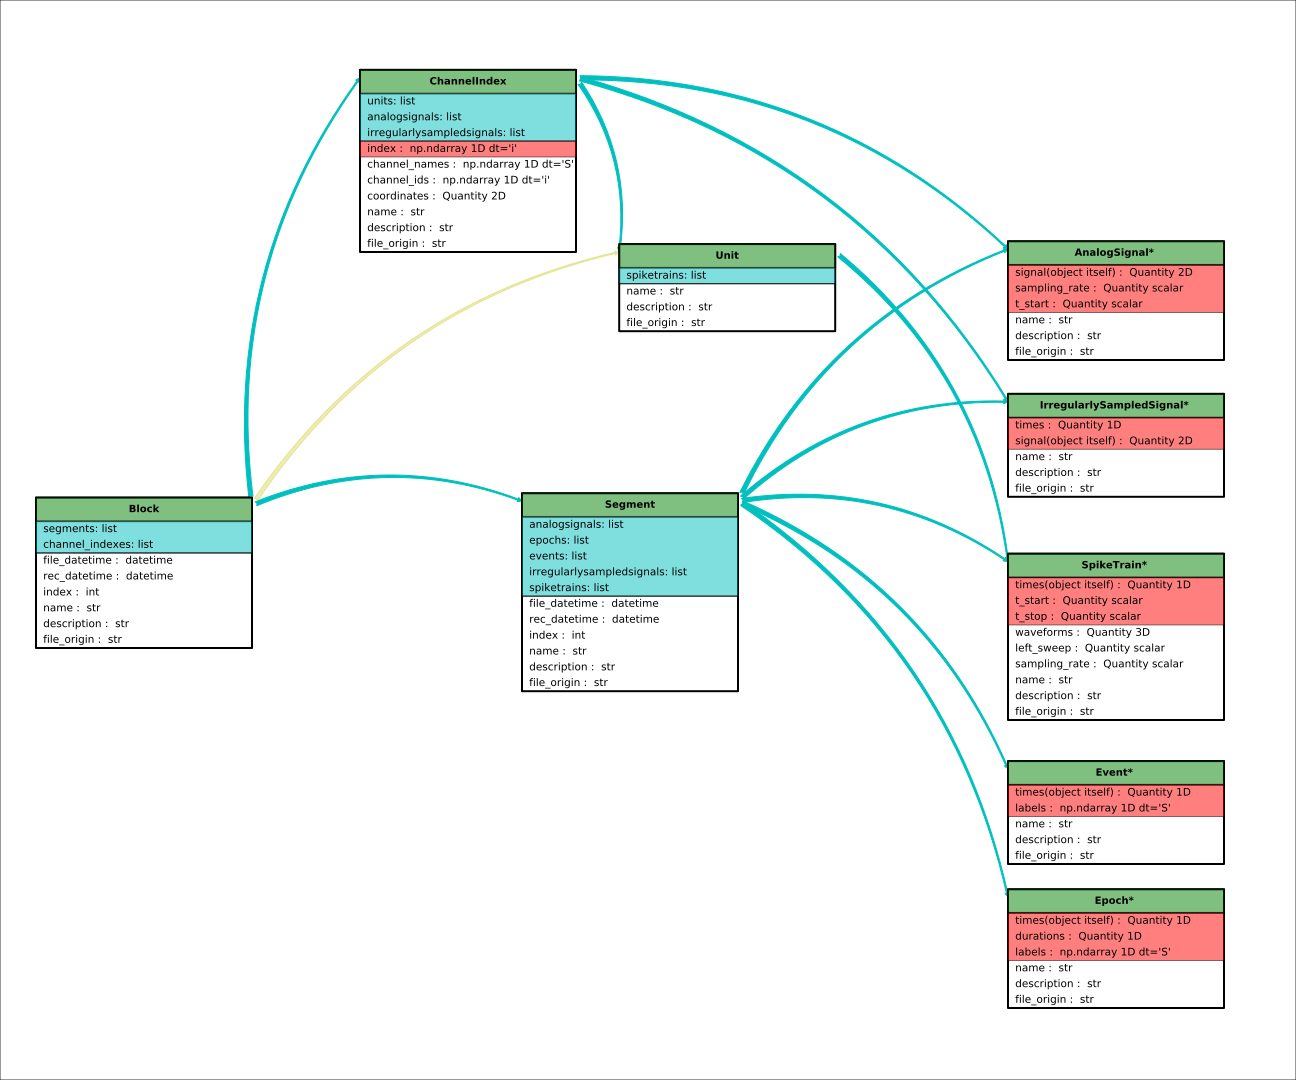
\includegraphics[width=\textwidth]{./Figures/simple_generated_diagram.png}
    \label{fig:neo_uml}
    \caption{Neo 0.7 object structure. Figure modified from \url{https://github.com/neuralensemble/python-neo}.}
\end{figure}


\begin{figure}
    \centering
    \def\svgwidth{\textwidth}
    \input{./Figures/neo_architecture7.tex}
    \label{fig:neo_architecture}
    \caption{Neo 0.7 architecture. Neo represents electrophysiology signals in data objects such as \code{AnalogSignal}s, \code{IrregularlySampledSignal}s and \code{SpikeTrain}s optionally including information about waveform data for each spike. Additional supplementary information describing the timing during the recording can be provided using \code{Event}s or \code{Epoch}s to mark time points or durations during the recording, respectively. All above described data objects are put into relation by container objects, such as \code{Segment}s (grouping all data objects simultaneous in time), \code{Unit}s (grouping \code{SpikeTrain}s across time) and \code{ChannelIndex}es (grouping \code{AnalogSignal}s \code{IrregularlySampledSignal}s and \code{Unit}s). The top level container is a \code{Block} linking to \code{Segment}s and \code{ChannelIndex}es. Figure modified from \url{https://github.com/neuralensemble/python-neo}.}
\end{figure}


% ...
% \subsection{Exemplary Figure}
% \label{subsec:Section_Name/fig}
% ...
% \begin{figure}[htbp]
%     \centering
%     \includegraphics[width=.5\linewidth]{./Figures/UoC_Logo.png}
%     \caption{Exemplary Figure}
%     \label{fig:UoC}
% \end{figure}
% 
% 
% \subsection{Exemplary Figure Referencing}
% \label{subsec:Section_Name/fig_rfs}
% 
% See Figure \ref{fig:UoC} for details. Additional information can be
% found in the footnote \footnote{Image taken from \url{https://en.wikipedia.org/wiki/File:Siegel_Uni-Koeln_(Grau).svg}.}.

\clearpage
\chapter[Data representation]{Standardized data representations\\- Making data usable}
\label{sec:neo}
% importance of standardization and global organizations 
For making data interoperable 
For widely accepted and utilized and interoperable data storage and usage, as suggested by the FAIR principles for scientific data management \citep{Wilkinson_2016}, it is necessary to agree on common file formats for storage on disc as well as data representations in memory. The agreement on data standards can develop in a 1) community driven way by groups of users adopting a format and therefore forming the basis for a general spread of the format or 2) industry defined, by companies or organizations defining a standard. In the context of data storage and representation there are numerous standards already defined and maintained. For example the World Wide Web Consortium\footnote{W3C, \url{https://www.w3.org/}} is an international community, that is coordinating the development and maintenance of open standards to ensure the long-term growth of the internet. This includes e.g. the widely spread format scalable vector graphics (svg) format and the Hypertext Markup and Extensible Markup Languages (html, xml, respectively). These standards were developed in a community driven way, and are still continously improved by working groups\footnote{W3C working groups, \url{https://www.w3.org/Consortium/activities}} (e.g. the svg2 format\footnote{svg2, \url{https://www.w3.org/TR/SVG2/}}).


% why this doesn't cover smaller scientific fields
Standards as they are defined by the World Wide Web Consortium affect millions of users and computer systems. Therefore, the issue of standardization forms a foundation for a working system with this large number of participants. On smaller scales however the topic of standardization is not as pressing as individual members are typically able to develop a system, which meets their requirements and often does not require interaction with other systems. At the same time the complexity and specificity of the data and metadata to be represented increases since more detailed information needs to be captured and tracked in a consistent manner. This leads to a an unproportionally high effort required when interacting with other members of the community since the locally established implicite agreements on data storage and handling need to be communicated in addition to the actual data content.

% BIDS as positive example
One way even smaller communities can benefit from standardized data representations from an early stage on is the introduction of standards from the recording system manufacturing side. This situation is more likely to occur if only very few experimental systems exist (e.g. particle physics and the \code{root} format \citep{Brun_1996}) or only few manufacturers produce experimental setups, which simplifies the coordination between these (e.g. medical imaging and the Digital Imaging and COmmunications in Medicine (DICOM) standard\footnote{DICOM, \url{https://www.dicomstandard.org/}}). Based on this, the neuroimaging community managed to extend the standard to coherently organize metadata with data in the Brain Imaging Data Structure\footnote{BIDS, \url{https://bids.neuroimaging.io/}} \citep{Gorgolewski_2016}.

% standards as prerequisite for tool development and vice versa
Standards can emerge from a community or can be established by dominating entities, e.g. in case of a monopoly for hardware production. However, also the development of tools used within and across communities is tightly linked the definition of standards, as these form a prerequisite for interacting with the data. This interaction works both ways: the establishment of standards is important for the development of tools to enable them to get the most information out of the datasets, but also tools can influence the establishment of standards especially in small communities by favouring one format over another and therefore influencing the community preferences. The development of tools applicable across communities requires the prior adoption of global standards, as community internal evolved agreements are typically too diverse to be transferred to other communities to form a basis for a common set of tools. 

% neuroscience: state of the art
A prime example for the delayed recognition for the need of standardization is the development of data formats in the field of electrophysiology. Here specific requirements are needed for when recording electrophysiology datasets: The file formats need to be able to support writing of large amounts of data in a streaming fashion, they have to cope with the custom data structure generated by the recording system  and they need to document the parameters used during the recoding as minimal metadata. This, together with a number of companies developing ready-to-use solutions for experimentalists led to a multitude of file formats (see also \cref{fig:neo_ios}). All systems permit experimentalists to record data without investing years into the development of a recording system but also typically provide only very few supported output file formats. This again restricts the number of easily applicable analysis methods, as the vendor may provide tools for basic visualization, processing and simple analysis the data, but these are typicaly not easily extendable nor do they provide a simple programming interface for the implementation of custom analyses. This unnessarily restricts the scientific questions which can be answered with a particular dataset based on the producer of the hardware system.\\

% neuroshare
A project introducing a common output file format for electrophysiology recording systems is Neuroshare \footnote{Neuroshare, \url{http://neuroshare.org/}}. Version 1.0 was released in 2003 and is a C based library relying on direct-link libraries for the integration with recording systems and providing scripts for the integration in a \software{Matlab} environment. However, neuroshare was only taken up by few vendors of electrophysiology setups, as these are required to provide integration routines for their acquisition system. Additionally, the Neuroshare was mainly developed for Windows based systems, making it complicated to use in combination with other operating systems. In 2010 a Python implementation of Neuroshare was introduced\footnote{python-neuroshare, \url{https://github.com/G-Node/python-neuroshare}}, which is currently not maintained.

Since then, multiple projects attempt to tackle this problem from different angles: The Neurodata Without Borders: Neurophysiology\footnote{\software{NWB:N}, \url{https://www.nwb.org/}} \citep{Teeters_2015} project attempts to define an additional, more generic file format standard aiming to replace a multitude of existing formats. This project was launched in 2014 and a second version was released in 2019 \citep{Rubel_2019}. The project involved multiple scientific laboratories, funding agencies as well as industry partners and provides a fixed set of structures to describe common data encounterd in this collaboration. The \software{NWB:N} format is not supported by major recording setup manufacturers and therefore no file format generated by common electrophysiological recording setups. Instead primary recording data need to be converted into the \software{NWB:N} format.
Another project tackling the same problem is the Python package \software{Neo}. \software{Neo} is a spin-off of the \software{Neurotools} toolbox, an attempt to set up a common file format for neurophysiology setups based on Microsoft dynamic-link libraries. It was initiated in 2009 and in contrast to NWB provides a standardized in memory data representation for electrophysiology data without introducing another file format. Therefore it bridges the gap between available electrophysiology file formats and forms the basis for a number of visualization, preprocessing and analysis tools. By interfacing to a large number of file formats \software{Neo} is the ideal tool for implementing flexible data management workflows independent of the particular file format of the original data files. In addition, it provides also flexibility in the range of software tools that can be used for further data processing as it interfaces with various tools that cover diverse requirements of data processing, visualization and analysis. In the following we will introduce \software{Neo} in more detail and provide example scripts for application of \software{Neo} for handling electrophysiology datasets.



\section{The \software{Neo} Python Package}
\software{Neo}\footnote{\software{Neo}, \url{http://neuralensemble.org/neo}, RRID:SCR\_000634} \citep{Garcia_2014} is an open-source Python package for representing electrophysiology data in working memory. It offers interfaces for reading various electrophysiological proprietary and open file formats and represents the data in a generic way (\cref{fig:neo_ios}). Thus it forms the bases for a number of open software tools: The electrophysiology analysis toolkit\footnote{Elephant, \url{http://neuralensemble.org/elephant}, RRID:SCR\_003833} for analysis of spiking activity and local field potentials, OpenElectrophy\footnote{OpenElectrophy, \url{http://neuralensemble.org/OpenElectrophy}, RRID:SCR\_000819}, SpykeViewer\footnote{SpykeViewer, \url{https://spyke-viewer.readthedocs.io}} and Ephyviewer\footnote{Ephyviewer, \url{https://ephyviewer.readthedocs.io}} for visualization, Tridesclous\footnote{Tridesclous, \url{https://tridesclous.readthedocs.io}} for online and offline spike sorting, NeoAnalysis\footnote{NeoAnalysis, \url{https://github.com/neoanalysis/NeoAnalysis}} \citep{Zhang_2017} for rudimentary visualization and analysis, NetworkUnit \footnote{NetworkUnit, \url{https://github.com/INM-6/NetworkUnit}, RRID:SCR\_016543} for validation testing of spiking networks. Related packages are \software{NiBabel}\footnote{NiBabel, \url{https://nipy.org/nibabel}, RRID:SCR\_002498}, a comparable package for neuroimaging file formats and \software{MNE}\footnote{MNE, \url{https://martinos.org/mne}, RRID:SCR\_005972} an Python package for MEG and EEG analysis and visualization.

The two main features of \software{Neo} are 1) the interfacing to many different file formats, by providing reading capability for numerous proprietary formats and writing capability to selected open formats and 2) the standardized representation of electrophysiology data as a basis for further visualization and analysis steps. Using these features of \software{Neo} is typically used either as conversion tool from specialized to more generic formats or as run time data representation for further processing.

\subsection{Feature updates and current development}
The \software{Neo} version 0.3 was released in 2014 \citep{Garcia_2014}. Since then the software has been extended to be compatible with more data formats, the object model has been revised for better usability and the implementation has been improved for performance. In the following we describe the enhancements introduced between version 0.3 (\cref{fig:neo_architecture03}) and version 0.7 (\cref{fig:neo_architecture07}).

\paragraph{Interfaces to file formats}
\software{Neo} 0.7 is supporting additional file formats for reading, such as Axograph, OpenEphys, Stimfit, Kwik, Nix, Igor, Nest, Neuralynx, NSDF and BCI2000. The capabilities for reading the Axon, Blackrock, Brainvision, Brainware, Elphy, Intan Matlab structures, Neuroshare, Plexon, Spike2, Tdt, NeuroExplorer, Neuralynx, Igor, Elan, Micromed, RawMCS, WinWCP formats have been improved. Reading and writing capabilities have been improved for Nix and Pickle formats. PyNNText and PyNNNumpy formats are no longer supported. A new code design for readers has been implemented and the majority of readers has adjusted accordingly to enable improved loading performance and loading of subsets of data (RawIO implementation). 
\paragraph{Object structure and usability}
The code has been modularized for more flexibility and maintainability, and a large number of unittests have been added. The object structure has been restructured for user friendliness and to boost performance by implementing sets of similar data entities in single objects instead of using individual data objects for each data entity (removal of dedicated array versions of data classes). A new relational container object \code{Channel\_Index} was introduced to simplify the representation of logical relations between data objects replacing \code{RecordingChannel} and \code{RecordingChannelGroup} objects. Consistent deep copy functionality has been added for all data objects and additional internal consistency checks have been added. A new type of custom annotation mechanism has been added, which is designed to capture custom annotations in the same dimension as the data (array annotations). For the installation additional option were introduced, depending on the required file formats which need to be supported. The code style has been adjusted to follow the PEP8 guideline\footnote{Python Enhancement Proposal 8, \url{https://www.python.org/dev/peps/pep-0008}}\citep{PEP8StyleGuideforPythonCode_}. Support for Python 2.6 was dropped and consistent support for Python 3 was introduced.


\paragraph{Outlook}
Practical application of \software{Neo} confirmed an improved usability for version 0.7. The described data objects facilitate data access and performance and the combination of \code{Block} and \code{Segment} objects as container objects provides easy to use access to the data. However, the concept of \code{ChannelIndex} objects is covering too many aspects of relations between data at once: 1) grouping data objects, 2) masking data objects (selection of a subset of data within a data object) and 3) annotating individual samples within data objects. The last aspect has been moved to the individual data objects, by introducing array annotations. 

% groups and views
For future versions, the splitting of \code{ChannelIndex} objects into two separate objects (\code{Group}, \code{View}) responsible for grouping and masking is planned. A \code{Group} object will be able to link different types of data objects, depending on its configuration. For example a \code{Group} object resembling a physical electrode will be able to link to a single \code{AnalogSignal} and multiple \code{Unit} objects. A \code{View} object can be used to refer to a subset of the data stored in a data object (e.g. a single recording trace within an \code{AnalogSignal}). This view can be used instead of a data object in any relation and will provide utility functionality to provide a sliced version of the actual data object.

%linking
Another topic of discussion is the linking between \software{Neo} objects. Up to the current version 0.7 all links between \software{Neo} objects can be established bidirectional. However, the bidirectionality of the linking is not inherently guaranteed, since the generation of link does not automatically generate a backward link between \software{Neo} objects. Introducing automatic bidirectional linking would guarantee bidirectional linking, but might complicate the set up of a \software{Neo} structure e.g. when reading a data file. There are different approaches possible to circumvent these problems: i) The use of only unidirectional links from higher level to lower level objects (top to bottom). This approach would still provide most of the functionality commonly used. ii) The implementation of a validation framework, which can on request check if a provided \software{Neo} object structure is fully linked including consistent bidirectional links. A suggested model implementing the first of the two suggestions is presented in \cref{fig:neo_architecture_future}. Here links from \code{View}s and \code{Group}s towards data objects are unidirectional, therefore preventing cyclic links across the complete \software{Neo} structure.

%Imaging data
Spiking activity of individual neurons can not only be recorded using sharp electrodes, but also  from multielectrodearray recordings (MEA) and calcium image recordings \citep{Kelly_2007, Shew_2010}. To support the usage of \software{Neo} also for imaging data an extension of \software{Neo} by two additional object types is planned: the \code{ImageSequence} object will capture sequences of regularly sampled images and is therefore closely related to the \code{AnalogSignal} as it contains the same type of data, but also captures the spatial relation between different pixels (traces). A second object relevant for image handling is a \code{RegionOfInterest} object, which is used to spatially mask a specific part of a stack of images. The \code{RegionOfInterest} can implemented as special case of a \code{View}. Support for \code{ImageSequence}s also requires capabilities to read imaging data formats, which will be added subsequently.


\subsection{\software{Neo} Object Structure}
% data vs container objects, general attributes: name, description, file\_origin
\software{Neo} objects can be separated into two types: data objects, describing basic recording data in combination with minimal metadata and container objects, providing the structural framework for the relation between the data objects. In general, all \software{Neo} objects have three optional arguments to provide custom information about the captured data: 1) \code{name} attribute can be used to label the object and can be used for simple data filtering and selection. 2) The \code{description} attribute is intended to provide a human readable, detailed, 1-2 sentence description for the data contained / grouped by the \software{Neo} object. The \code{file\_origin} is can be used to describe the origin of the data, e.g. the original recording filename or simulation script. In addition to \code{name}, \code{description} and \code{file\_origin}, all \software{Neo} objects can capture additional custom information in form of a \code{annotation} dictionary. This dictionary can contain arbitrary data in all basic Python data types as well as \code{datetime}, \code{date}, \code{time}, \code{timedelta} in arbitrary structures build from lists, dictionaries, tuples or \software{Numpy} arrays without any restrictions on the shape of these objects.


\paragraph{Data Objects}
Data objects are based on \software{Numpy} arrays \citep{Walt_2011} for efficient computation on large datasets. In addition, \software{Neo} objects are aware of physical quantities by using the \software{Quantities} package \citep{Dale_}.
% Continuously Sampled Signals
\software{Neo} provides data objects to capture regularly as well as irregularly sampled continuous signals in \code{AnalogSignal} and \code{IrregularlySampledSignal} objects, respectively. Both objects rely on a 2 dimensional \software{Quantities} (\software{Numpy}) array capturing the basic data signal, whereas the first dimension describes the time and the second dimension different signal traces. For \code{IrregularlySampledSignal}s time information is captured in a second separate \software{Quantities} array, sharing the first dimension with the signal array. For \code{AnalogSignal}s this in implemented in a more compact fashion by storing only the sampling rate (\code{sampling\_rate}) and the starting time point of the recording (\code{t\_start}). A \software{Quantities} array containing the time values corresponding to the data point can be generated on request via the \code{times} attribute of the \code{AnalogSignal}.
% Time series data
For time series data \software{Neo} provides a \code{SpikeTrain} object, capturing the data in a \code{times} attribute. Additionally the start and stop times of the data acquisition are essential for the interpretation of the data, these are provided as mandatory \code{t\_start} and \code{t\_stop} scalar \software{Quantities} parameters. Optionally, a \code{SpikeTrain} object can also capture snippets of regularly sampled continuous signal around each time point in the waveform attribute. This links to a 3 dimensional array, capturing the time, spike ID and recording channel dimensions of the waveforms. The \code{SpikeTrain} attribute \code{sampling\_rate} is used to capture the corresponding sampling information as in the \code{AnalogSignal} case. To relate the waveform snippets with the time series data the \software{Quantities} scalar \code{left\_sweep} defines the constant offset between the time series data and the corresponding waveform snippet.
% Events and Epochs
A different type of time series data is non-neuronal time series which describe specific time points or durations during the recording of neuronal activity. These might be control signals of the experiment, e.g. trial start times, behavioral events of the subject, e.g. a the time in which a button was pressed. For the description of time series data \software{Neo} provides \code{Event} objects, capturing the data in a one dimensional \software{Quantities} array (\code{times} attribute) together with a string array of the same shape (\code{labels} attribute) providing labels to the individual time points. To represent extended periods of time, \software{Neo} offers \code{Epoch} objects having the same attributes as \code{Event}s, and in addition a one dimensional \software{Quantities} array of durations with the same shape as the main time series data.

% Array annotations
All of the above mentioned data objects consist of a main \software{Quantities}-wrapped \software{Numpy} array with one or more dimensions. One of the latest features introduced in \software{Neo} is to implement a second kind of annotation mechanisms on this. The annotations of an object always refer to the object as a whole. However in many use cases annotations have been used to provide details about the individual data samples by containing arrays, which share some dimensions with the main data samples. For example \code{AnalogSignals} which contain more than one recording trace are frequenly annotated with list providing detailed information about the individual recording channels, e.g. the identity of the channel or the particular filter settings. However, when modifying the shape of the original data, these annotations can not be updated in an automatic fashion since they were user defined and didn't follow a fixed schema. Since \software{Neo} version 0.7.0 all data objects have an additional feature \code{array\_annotation}s, which fills this gap by providing an annotation mechanism for capturing sample based annotations, i.e. annotation entries with the same length as the main data dimension. These \code{array\_annotations} are automatically adjusted when the shape of the main data is modified, e.g. by slicing the data in the time axis or extracting a single signal trace from an \code{AnalogSignal}.

% Lazy loading
The \code{Neo} 0.7 release also features a standardized way of optionally loading specific parts of the data on request. This is of advantage when dealing with datasets which are large in comparison to the available memory. The new \code{lazy} feature permits to generate the complete \software{Neo} structure (\cref{fig:neo_architecture07}), but substituting all data objects with proxy objects, which feature the same attributes and links as classic data objects, but do not contain the actual data. For accessing the data a \code{load} mechanism is provided which loads the requested parts of the data and provides them in a separate classic data object not linked to the main \software{Neo} structure. Using the \code{lazy} mechanism large datasets can be processed chunkwise without requiring large amounts of memory.

\paragraph{Container Objects}
% Block and Segment
\software{Neo} container objects provide the structural relations between \software{Neo} data objects. The base object for a dataset is a \code{Block} object, containing everything related to the dataset. The \code{Block} object can link to a number of \code{Segments} and \code{ChannelIndex} objects which can be used to organize data objects according to their timing, spatial relation or custom grouping aspects, e.g. grouping the data objects by the signal quality of the contained data. \code{Segment} objects are intended for grouping objects which share the same time frame, e.g. simultaneously recorded \code{AnalogSignal}s and \code{SpikeTrain}s (\cref{fig:neo_architecture07}).
\code{SpikeTrain}s from different \code{Segment}s that are considered coming from the same source (neuron) can be linked across \code{Segments} via \code{Unit} objects.
% Units and ChannelIndexes
A \code{Unit} object again can be grouped together with \code{AnalogSignal}s and \code{IrregularlySampledSignal}s in a \code{ChannelIndex} object. In addition to the grouping functionality, a \code{ChannelIndex} object also provides an additional labeling functionality for child \code{AnalogSignal}s via the \code{channel\_ids} and \code{channel\_names} attributes. These consist of one dimensional integer and string arrays labeling the individual traces of the attached continuous signals. Via the mandatory attribute \code{index} a selection of the traces within the linked continuous signals can be done. However, this requires a consistent ordering of recording traces within all linked continuous signals of a \code{ChannelIndex}.
All container objects provide utility functions to facilitate access and selection of data objects. This is implemented in the form of a \code{filter} method, which returns a list of \software{Neo} objects based on a combination of object type, attribute and annotation constraints.


\begin{figure}
    \centering
    \includestandalone[mode=image|tex, width=\textwidth, obeyclassoptions=true]{./figures/neo_ios_and_tools}
    \caption[Neo embedding]{\software{Neo} embedding. \software{Neo} 0.7. supports a number of file formats for reading (light blue) and writing (dark blue). Many of the supported formats can be read in a improved fashion, permitting for more efficient memory usage (black frames).  Neo provides an interface for many advanced tools for visualization, simulation, analysis and data storage.}
    \label{fig:neo_ios}
\end{figure}


\begin{figure}
    \centering
    \includesvg[width=\textwidth,pretex=\relscale{0.8}]{./figures/neo07_schema.svg}
    \caption[\software{Neo} 0.7 object structure]{\software{Neo} 0.7 object structure. Figure modified from \url{https://github.com/neuralensemble/python-neo}.}
    \label{fig:neo_uml}
\end{figure}

\begin{figure}
    \centering
    \software{Neo} 0.3 architecture
    \includesvg[width=\textwidth]{./figures/neo_architecture03.svg}
    \caption[\software{Neo} 0.3 architecture]{\software{Neo} 0.3 architecture. \software{Neo} represents electrophysiology signals in data objects such as \code{AnalogSignal}s, \code{AnalogSignalArray}s, \code{IrregularlySampledSignal}s, \code{SpikeTrain}s and \code{Spike}s, whereas the latter two optionally include information about waveform data for each spike. Additional supplementary information describing the timing during the recording can be provided using \code{Event}s and \code{EventArray}s or \code{Epoch}s and \code{EpochArray}s to mark time points or durations during the recording, respectively. All above described data objects are put into relation by container objects, such as \code{Segment}s (grouping all data objects simultaneous in time), \code{Unit}s (grouping \code{SpikeTrain}s and \code{Spike}s across time), and \code{RecordingChannel}s and \code{RecordingChannelGroup}s (grouping \code{AnalogSignal}s \code{IrregularlySampledSignal}s and \code{Unit}s, \code{AnalogSignalArray}s and \code{RecordingChannel}s, respectively). The top level container is a \code{Block} linking to \code{Segment}s and \code{RecordingChannelGroup}s. Figure from \url{https://neo.readthedocs.io/en/0.3.3}.}
    \label{fig:neo_architecture03}
\end{figure}


\begin{figure}
    \centering
    \includesvg[width=\textwidth]{./figures/neo_architecture07.svg}
    \caption[\software{Neo} 0.7 architecture]{\software{Neo} 0.7 architecture. \software{Neo} represents electrophysiology signals in data objects such as \code{AnalogSignal}s, \code{IrregularlySampledSignal}s and \code{SpikeTrain}s optionally including information about waveform data for each spike. Additional supplementary information describing the timing during the recording can be provided using \code{Event}s or \code{Epoch}s to mark time points or durations during the recording, respectively. All above described data objects are put into relation by container objects, such as \code{Segment}s (grouping all data objects simultaneous in time), \code{Unit}s (grouping \code{SpikeTrain}s across time) and \code{ChannelIndex}es (grouping \code{AnalogSignal}s \code{IrregularlySampledSignal}s and \code{Unit}s). The top level container is a \code{Block} linking to \code{Segment}s and \code{ChannelIndex}es. Figure modified from \url{https://github.com/neuralensemble/python-neo}.}
    \label{fig:neo_architecture07}
\end{figure}


\begin{figure}
    \centering
    \includesvg[width=\textwidth]{./figures/neo_architecture_future.svg}
    \caption[Proposed \software{Neo} architecture]{Proposed \software{Neo} architecture. The proposed \software{Neo} architecture preserves all objects from \software{Neo} version 0.7 except for \code{ChannelIndex}es and \code{Unit}s. These are replaced by \code{Group} and \code{View} objects, which a more generic, but still customizable way of organizing data objects. \code{View} objects can mask data objects by linking to a subset of the contained data (e.g. a single trace of an \code{AnalogSignal}. This linking is unidirectional, preventing complex dependencies involving data objects. \code{Group}s are capable of linking to any kind of data objects or \code{View} of data objects. The required specificity is provided by the different \code{mode}s of a \code{Group} object. These limit to the connected objects to a specific type and number, wherefore a \code{Group} can e.g. be used instead of a \code{Unit} object. \code{Group}s can also link to other \code{Group} objects to provide higher level organization of the data.}
    \label{fig:neo_architecture_future}
\end{figure}


\section{\software{Neo} Usage Examples}
In the following we demonstrate in three practical examples how \software{Neo} can be used to load data from different file formats in a memory efficient manner, access and select data, annotate and filter data according to custom metadata added and save data in an open source format.

\subsection{Loading \& Visualization}
Loading data in \software{Neo} is implemented in two stages: First initialization of the reader (IO) and second reading of the \software{Neo} structure. For readers implemented in the standardized manner (\cref{fig:neo_ios}, black frame) you need to provide the filename of the dataset to load. This will generate an \code{io} object providing functionality to load the data into a \software{Neo} structure. Depending on the file format either a \software{Neo} \code{Block} or a \software{Neo} \code{Segment} can be loaded using the \code{read\_block} or \code{read\_segment} method of the \code{io} object.

In this example, the published dataset described in \cref{sec:data} is used for demonstrating the loading of electrophysiology data into the \software{Neo} structure (\cref{code:neo_visualization}). Data were previously downloaded from GIN\footnote{\url{https://gin.g-node.org/INT/multielectrode_grasp}} and continuous as well as sorted spiking data are loaded using the \software{Neo} \code{BlackrockIO} class. This IO provides standardized access to the data, permitting lazy loading of \software{Neo} objects [cf. \cref{code:neo_visualization} line 10f]. Here the the \software{Neo} filter functionality is used to select all \code{SpikeTrain}s which have an annotation key \code{'channel\_id'} and the corresponding value of the user requested channel index (\code{selected\_channel}, line 13). In the next step, the corresponding \code{AnalogSignal} trace is extracted by finding the \code{AnalogSignal} with a corresponding in the \code{array\_annotation} with key \code{channel\_ids} and extracting the \code{id} of the corresponding trace (line 15-18). Finally, the analog and spiking data of 10 seconds of recording are loaded into memory via the \code{load} mechanism of the respective data objects and returned by the \code{load\_single\_channel\_data} function (line 19-22).

The visualization of a single \code{AnalogSignal} trace together with spiking activity from multiple \code{SpikeTrain}s is implemented in the \code{plot\_data} function. This requires the corresponding data objects as input as well as a location to store the final scalable vector graphics plot (line 25). Here, \software{Matplotlib} \citep{Hunter_2007} is exploited to visualize the electrophysiological data (line 30 \& 34-38). Correct scaling of the signals and automatic generation of axis labels is ensured by the inherent use of the \software{Quantities} package within \software{Neo} (line 28-31, 34-37). The resulting plot is exported to the scalable vector graphics (svg) format for storage in a flexible, memory efficient and scalable manner. Finally, user specific setting are extracted from command line parameters and both functions are executed sequentially to generate a visualization of a single recording trace and corresponding spiking activity.




\begin{codeenv}
\inputminted[linenos,tabsize=2,breaklines, fontsize=\scriptsize]{python}{figures/code_visualize_data.py}
\caption[Data loading and visualization with \software{Neo}]{Loading data into the \code{Neo} framework and visualization using the Matplotlib package. Required packages are imported (line 1-4) and two main functions are defined for loading and visualization of the \software{Neo} structure: \code{load\_single\_channel\_data} and \code{plot\_data}. The first one requires the location of the datasets and the selected channel to plot as command line arguments (line 9). Here, the dataset is opened using the \code{BlackrockIO} in \code{lazy} mode and the user-specified channel is selected and loaded into memory together with the spiking activity (lines 7-22). The second function visualized a given \code{AnalogSignal} together with a list of \code{SpikeTrain}s using the \software{Matplotlib} package (line 25-40). Finally both functions are run subsequently using command line parameters for dataset and channel specifications. For the resulting plot see
\cref{fig:demo_visualization}}.
\label[codelisting]{code:neo_visualization}
\end{codeenv}

\begin{figure}
    \centering
    \includesvg[width=\textwidth]{./figures/i140703-001.svg}
    \caption[Data visualization example]{Visualizating of the activity recorded on a single electrode. A single trace of an AnalogSignals contains the voltage samples of a recording electrode (blue). The corresponding threshold crossing events are split into three different \code{SpikeTrain} objects and time stamps are marked as vertical lines with a \code{Unit} specific offset (orange, green, red).}
    \label{fig:demo_visualization}
\end{figure}

\subsection{Annotation of data with metadata from \software{odML}}
Annotations are a key feature of the generic \software{Neo} structure to provide the necessary customizations to be used for a specific dataset. Standard annotations are a feature of all \software{Neo} objects and can be accessed via the \code{annotation} attribute. In addition, \software{Neo} data objects also provide a more specific type of annotation mechanism, namely \code{array\_annotations} which act in the same manner as regular \code{annotations} but are directly coupled to the dimension of the underlying data. This permits to store metadata which are linked to individual data entries and handle them in an automatic way when manipulating the data object. This example demonstrates how to access and modify regular and array annotations using a metadata collection in the odML format.

\cref{code:neo_annotation} demonstrates two aspects of \software{Neo} annotations: firstly annotation access via the object attributes \code{annotation} and \code{array\_annotation} and secondly the generation of (array) annotations. The resulting script output is shown in \cref{code:neo_annotation_print}. The dataset is loaded in the same manner as in \cref{code:neo_visualization} and \code{annotations} and \code{array\_annotations} of selected objects are printed using the \code{print\_annotations\_example} functions. The resulting printout shows the different levels of annotations, which are automatically generated by \software{Neo} when loading a dataset from the \code{Blackrock} format. Annotations on the \code{Block} level provide general information about the recording session, whereas \code{SpikeTrain}s carry very specific metadata about the identity of the object and its spike sorting classification.

An example for \code{array\_annotations} is provided for an \code{AnalogSignal}. \code{AnalogSignal} objects provide the most metadata as they describe all recording traces they contain individually (see \cref{code:neo_annotation_print} line 15-33). Here the \code{AnalogSignal} contains 96 recording traces and all array annotations have a matching length of 96. The annotated information covers the identity of the electrodes ('channel\_ids' and 'channel\_names', line 16f) and identity within the recording system ('connector\_ID' and 'connector\_pinID', line 19f) as well as signal processing parameters for signal filtering and spike extraction (line 21-30). Here the keys consist of a combination of the file type affected (nsx/nev), the filter border (high/low), the general parameters (freq/energy\_threshold/dig(itization)\_factor/waveform\_size) and filter parameters affected (corner/order/type). In addition, a human readable description as well as information about the originatign file is provided ('description', 'nsx' and 'file\_origin', line 18, 31f). All \code{array\_annotations} will automatically be adjusted when the underlying data object is modified via \software{Neo} functions, e.g. via slicing in time.

The second part of the example script (\cref{code:neo_annotation}, line 28ff) demonstrates the generation of additional (array) annotations by loading a metadata collection in the odML format, extracting relevant information for the interpretation of an \code{AnalogSignal} and adding this information to the \code{AnalogSignal} as array annotation. First, an odML file is loaded using the Python \software{odML} library (line 31) and all \code{Sections} describing electrodes are extracted to load a mapping between the Blacrock channel \code{ID}s provided by the recording system and the spatially ordered \code{ConnectorAlignedID}s (line 32f), which are defined in order to indicate an electrode's spatial position easily. In the next step, the existing Blackrock \code{ID} array annotations of an \code{AnalogSignal} are used to generate the corresponding array of \code{ConnectorAlignedID}s using the previously extracted mapping b(line 36f). Finally, the new ids are added as a new array annotation to the \code{AnalogSignal} using the \code{array\_annotate} mechanism (line 38).

The generated array annotations are displayed by printing the complete array annotations of the \code{AnalogSignal} again, resulting in \cref{code:neo_annotation_print} line 43ff. Here, the new key 'connector\_aligned\_ids appears containing the corresponding spatially organized ids of the recording electrodes.

With array annotations and annotations, \software{Neo} now offers a mechanisms to provide custom information for \software{Neo} objects as a whole, but also for subsets of data contained by \software{Neo} objects. With these annotation mechanisms it is now possible to directly add \software{odML} content to \software{Neo} objects on multiple levels of the data organization. However, this annotations are not automatically generated yet, since there is no mechanism assigning data in the \software{Neo} structure and metadata in the \software{odML} structure. Due to the generality of \software{Neo} and \software{odML} structure the is no generic assignment strategy between the two structures possible, but these relations need to be captured explicitely using an extended framework.


\begin{codeenv}
\inputminted[linenos,tabsize=2,breaklines, fontsize=\scriptsize]{python}{figures/code_annotate_data.py}
\caption[Annotation access and editing with \software{odML} and \software{Neo}]{Annotation access and editing with \software{odML} and \software{Neo}. Required packages are imported (line 1) and three functions for printing \code{annotations} and \code{array\_annotations} are defined (line 3-25). \code{pretty\_print\_dict} provides functionality for displaying individual dictionary items in separate lines (line 3-6). \code{print\_annotations} uses the previous function to print based on the \code{mode} keyword the \code{annotations} or \code{array\_annotations} of a given \software{Neo} object. \code{print\_annotation\_example} prints a selection of \code{annotations} and \code{arra\_annotations} from a \software{Neo} block structure. The function \code{generate\_annotations\_from\_odml} extracts metadata information about the mapping of different types of \code{id}s from an \code{odML} file and annotates the corresponding \code{AnalogSignal} (line 27-37). Finally, all functions are demonstrated based on a command line specified data- and metadataset (\code{data\_location} and \code{odml\_filename}, line 40-45). The generated annotations are confirmed via a final call of \code{print\_annotations} (line 46f).}
\label[codelisting]{code:neo_annotation}
\end{codeenv}

\begin{codeenv}
\inputminted[linenos,tabsize=2, fontsize=\scriptsize, style=friendly]{cucumber}{figures/i140703-001_annotations.txt}
\caption[Output of \cref{code:neo_annotation}]{Output of  \cref{code:neo_annotation}. Listed are the automatically generated annotations of example \software{Neo} objects as extracted from \code{Blackrock} recording files. On the \code{Block} level these are dealing with general information about available files and interruptions in the recording process. For \code{SpikeTrain}s there is information provided about the identity and classification of the \code{Unit} the \code{SpikeTrain} was assigned to. For \code{AnalogSignal}s there are a arrays describing the attributes of the individual electrode traces. This includes information about the electrode identities (\code{channel\_ids}), mappings of contacts within the recording system (\code{connector\_ID}s, \code{connector\_binID}s) and the applied filter and threshold settings for signal preprocessing and spike extraction.}
\label[codelisting]{code:neo_annotation_print}
\end{codeenv}


\subsection{Saving Data \& Format Conversion}
\label{sec:nix_format}
Being able to store intermediate preprocessing steps or analysis results in a persistent manner is important for making workflows reproducible. \software{Neo} provides the option to store data in plain Ascii, KlustaKwik \citep{Hazan_2006}, Nix \citep{Stoewer_2014}, binary Matlab, Neuroscience Simulation Data Format (NSDF) \citep{Ray_2016}, binary Python pickle and a custom binary format, see also \cref{fig:neo_ios}. In this example we focus on the Nix format as it provides the most versatile data storage. Nix is based on an hdf5 \citep{TheHDFGroup_1997} backend which provides the flexibility of fast and memory efficient access for large datasets. In addition, Nix is designed to capture data as well as metadata, providing the opportunity to unify both in a single file and add links between relevant metadata and the corresponding data. 
This example demonstrates the conversion of the dataset used already in previous examples from the \code{Blackrock} format to the \software{Nix} format. Furthermore, it showcases the addition of metadata from the \code{odML} format to the same file and the extraction of the data from the \software{Nix} file.
\cref{code:neo_saving} provides four functions for the back and forth conversion of files in the \software{Neo} and \software{odML} format to the \software{Nix} format (line 4-24). These functions are mostly based on the open-source \software{nix-odML-converter} library \footnote{\url{https://github.com/G-Node/nix-odML-converter}}. This library can be used for simple command line conversion between \software{Nix} and \software{odML}. Here we demonstrate the usage of the Python interface, permitting a more flexible approach to conversion parameters (e.g. filenames, write modes).
We demonstrate the merging of the data together with the metadata into a single \software{Nix} file using the first two functions (\cref{code:neo_saving} \code{save\_neo\_to\_nix} and \code{save\_odml\_to\_nix}). The last two functions deal with the extraction of the corresponding information of the individual components from the \code{Nix} file (\cref{code:neo_saving} \code{load\_odml\_from\_nix} and \code{load\_neo\_block\_from\_nix}).

With the capability of the \software{Nix} format to capture data as well as metadata in a combined fashion both modalities can be comprehensively stored in a common framework. Integrating both modalities in the \software{Nix} format is easy since \software{Neo} is supports the writing of data in the \software{Nix} format and metadata can be supplemented using the \software{nix-odML-converter}.

\begin{codeenv}
\inputminted[linenos,tabsize=2, fontsize=\scriptsize]{bash}{figures/code_saving_data.py}
\caption[Saving data and metadata to \software{NIX}]{Saving data and metadata to \software{NIX}. Required packages are imported (line 1f) and four functions for the conversion between \software{Neo} and \software{odML} on the one side and \software{Nix} on the other side are defined (line 4-24). The main part of the script (line 26ff) first extract command line specified parameters (location of the dataset and \software{odML} and \software{Nix} filenames to be used) and loads the datasets from the \code{Blackrock} format. Next, the \software{Neo} block in converted to the \software{Nix} format (line32) and the complete metadata collection is added from an \software{odML} file (line33). Finally, we demonstrate how to extract the corresponding information again from the \software{Nix} format using the \code{load\_odml\_from\_nix} and \code{load\_neo\_block\_from\_nix} functions (line36f). Please note that the execution time of this code highly depends on the size of the dataset, since for sequentially all parts the complete dataset will is loaded into memory.}
\label[codelisting]{code:neo_saving}
\end{codeenv}


\section{Comparison of \software{Neo} to \software{NWB:N}}
The \software{NWB:N} format \citep{Teeters_2015} is an alternative approach to \software{Neo} for handling of electrophysiology data. In contrast to \software{Neo} it specifies a new file format instead of providing interfaces to existing formats. More precisely, \software{NWB:N} provides a modular framework for the capture of specific electrophysiology modalities. %https://pynwb.readthedocs.io/en/stable/overview_software_architecture.html
It is accompanied by a number of canonical schema (type) for capturing specific types of data, e.g. behavioural and time series data, imaging recordings, extra and intracellular electrophysiology recordings as well as optogenetic stimulation and optical physiology. Custom schema can be specified to capture data modalities not covered by the set of canonical schema.  % https://nwb-schema.readthedocs.io/en/latest/
This makes the \software{NWB:N} format on the one side more generic than the \software{Neo} structure, since it permits the implementation of custom schema specifications, but on the other side also more restrictive, because existing schema specifications are very specific and can not be reused in a slightly different context. Also implementation of a custom schema specification extensions in \software{NWB:N} requires additional background knowledge of the experimenter about the underlying organization of the \software{NWB} package and the time and effort of implementing such a format. %https://nwb-schema.readthedocs.io/en/latest/format_description.html#extending-the-format
For \software{Neo} the approach is different: the underlying object structure is as generic to automatically cover most of the electrophysiology data and the experiment specificity is introduced via the annotation and array annotation mechanism. This implies that the user only has to understand the \software{Neo} objects once and can reuse the knowledge also in different experimental contexts.
\software{Neo} can deal with most of the available electrophysiology file formats and will be extended to cover calcium imaging data in the future. For \software{NWB:N} there are very limited conversion tools available to convert from specific \software{Matlab} structures and custom formats to the \software{NWB:N} format. %https://github.com/NeurodataWithoutBorders/exp2nwb  https://github.com/NeurodataWithoutBorders/mat2nwb https://github.com/NeurodataWithoutBorders/nwbn-conversion-tools
An interface for the support of additional formats exists, but format converters are in an early development stage. At this point \software{NWB:N} could benefit from integrating \software{Neo} to gain basic support for many electrophysiology formats.
\software{NWB:N} has reference implementations in Python as well as Matlab, suiting most of the neuroscientists, whereas \software{Neo} is only implemented in Python, focussing on non-commercial availability of electrophysiology analysis software.


\section{Summary}
We introduced the \software{Neo} Python package designed for standardized and efficient representation of electrophysiological data. We presented the development of the package since the original publication and depicted the main features and flexibility of the package in three small usage examples. Finally we provide a concise comparison to the recent \software{NWB:N} format and higlight the strengths of the software packages.
Using the \software{Neo} package provides a sound foundation for organizing research data according to the FAIR priniciples as \software{Neo} i) makes data accessible by supporting the conversion from various file formats to the standardized \software{Neo} data representation, ii) is an open, freely available und software package and iii) it makes data interoperable by providing a formal, accessible and broadly applicable basis for data representation. In addition \software{Neo} is supporting the \software{Nix} file format, which is fulfilling additional FAIR principles. These are i) making the data within the file format findable by using globally unique identifiers for data and metadata objects, ii) permiting the annotation with rich metadata as extensive metadata collections can be stored, iii) connecting data and metadata in a formal way by storing links between data and metadata objects, iv) being an open and free \& interoperable framework.
Additional aspects of the FAIR principles, like provenance tracking of the data and metadata, require the embedding of \software{Neo} and \software{Nix} in a data and metadata pipeline or workflow.



\clearpage
\chapter[Workflow management]{Workflow management\\- A new approach for research data and metadata management}
\label{sec:workflows}
The long process that starts from the generation of data, and ends in a scientific publication, can be separated into many individual steps. These subdivision may be coarse, like the separation only of experiment and subsequent analysis. Or they may be very fine, as each individual operation, and substeps within, may constitute and be implemented in independent processes.

Workflow management is the concept to organize these individual steps. The granularity of the steps to manage highly depends on the complexity of the tasks and the diversity of the processing steps. A common and generic example forming such a workflow management system (WMS) is a queuing system used in cluster computing such as \software{slurm}\footnote{slurm workload manager, \url{https://slurm.schedmd.com/}} or  \software{torque}\footnote{torque resource manager, \url{http://www.adaptivecomputing.com/products/torque/}} and \software{maui}\footnote{maui cluster scheduler, \url{http://www.adaptivecomputing.com/products/maui/}}. Here users submit a number of, in the simplest case, independent jobs (computing steps) which are then scheduled and distributed to suitable compute resources depending on the requested and available resources. This is a simple example, because the individual processing steps typically do not depend on each other and only the required amount of resources and time needs to be taken into account when organizing the execution. Already with these systems, it is possible to implement more complex scenarios, e.g. by defining an order of execution via dependency statements for individual jobs.

In this chapter we apply the concept of workflow management to solve the data and metadata management issues identified in \cref{sec:scidata_shortcomings}. A systematic workflow approach for data and metadata management supports the rigorous implementation of the FAIR principles, since the automation of processing steps relies to some extend on FAIR principles, i.e data should to have a unique identifier and should be organized in a structured fashion using standardized tools. Additionally, the implementation of a data and metadata workflow increases the reproducibility of the processing steps, as these are documented and provenance information can be tracked for each step of the workflow. Workflow management is suited to tackle the issues we identified in \cref{sec:scidata_shortcomings}, since it is designed to coordinate interdependent steps of a process as they occur in the data and metadata pipeline of the Reach-to-Grasp project. In the following, we present available WMSs and identify requirements for the applicability in the context of scientific projects in general as well as for Reach-to-Grasp and similar projects in particular.

For scientific projects like the Reach-to-Grasp experiment described in \cref{sec:data} there are dependencies between individual steps of the process from data acquisition to publication (see \cref{fig:scidata_metadata_pipeline,fig:scidata_reachgraspio_diagram}). The workflow management concept has been applied in a number of scientific fields like genomics or imaging data. In these fields a systematic approach to data processing and analysis is required and feasible, since they are dealing with large and numerous datasets which exceed manual monitoring or processing power \citep[e.g.][]{Palm_2010}.
For these and other disciplines, there are a number of platforms and tools available to implement pre \& post processing as well as analysis processing steps: Galaxy\footnote{Galaxy, \url{https://galaxyproject.org}, RRID:SCR\_006281}, an  open, web-based platform providing bioinformatics tools and services for data intensive genomics research; VisTrails\footnote{VisTrails, \url{https://www.vistrails.org}, RRID:SCR\_006261}, an open-source scientific workflow and provenance management system that provides support for simulations, data exploration and visualization; Taverna\footnote{Taverna, \url{https://taverna.incubator.apache.org}, RRID:SCR\_004437}, a scalable, open source \& domain independent tool for designing and executing workflows;  GenePattern\footnote{GenePattern, \url{http://www.broadinstitute.org/cancer/software/genepattern}, RRID:SCR\_003201}, a genomics analysis platform that provides access to hundreds of tools for gene expression analysis, SNP analysis, flow cytometry, RNA-seq analysis, and common data processing tasks; Renku\footnote{Renku, \url{https://datascience.ch/renku}}, an online software platform for reproducible and collaborative data science including workflow management aspects; Terra\footnote{\url{https://terra.bio/}}, a scalable platform  for biomedical research for data analysis and collaboration; Ugene \citep{Okonechnikov_2012} a multi platform open-source software for molecular biology; Luigi\footnote{Luigi, \url{https://luigi.readthedocs.io}}, a Python based tool for building complex pipelines of batch jobs; Airflow \footnote{Airflow, \url{https://airflow.apache.org/index.html}}, a platform programmatically author, schedule and monitor workflows; pinball\footnote{pinball, \url{https://github.com/pinterest/pinball}}, a scalable workflow manager with scheduling capability implemented in JavaScript and Python; make, a basic build automation tool available since 1976 with multiple implementations (e.g. gnumake\footnote{gnumake, \url{https://www.gnu.org/software/make/}}) and snakemake\footnote{Snakemake, \url{https://snakemake.readthedocs.io/en/stable/}, RRID:SCR\_003475}, a Python based language and execution environment for make-like workflows. 

In simple and straightforward projects, one may use plain bash scripts to coordinate the sequential execution of the individual steps of a workflows, mimicking a WMS. However, once the situations grows more complex, the same issues arise as discussed for the Reach-to-Grasp metadata pipeline (\cref{sec:scidata_shortcomings}): the bash script would form a monolithic script, trying to cover all possible dependencies between individual scripts resulting in overly complex code. Additionally, the script could only be executed all at once, without taking into account which steps of the workflow are actually required due to updates in the underlying sources files.

Scientific projects, such as the Reach-to-Grasp project presented in \cref{sec:data}, can benefit greatly from a structured workflow approach. However, the development of the workflow should in the best case smoothly integrate with the existing scientific tools and approaches used in the project. In the following, we discuss a number of essential features of a WMS, which are generally required in scientific projects. The WMS should 
\begin{quote}
\begin{description}
 \setlength{\itemsep}{5pt}
 \setlength{\parskip}{0pt}
 \setlength{\parsep}{0pt}
 \item[slim] not introduce unnecessary additional computational overhead
 \item[easy]  not require expert knowledge to implement and configure a workflow
 \item[standalone] not introduce additional unnecessary dependencies to other projects and programming languages
  \item[visual] be able to generate a visual overview of the workflow for inspection and debugging purposes
  \item[debuggable] be easy to debug
  \item[active] be actively supported
  \item[open] be open source and freely available\\
\end{description}
\end{quote}
Furthermore, we identify additional, more specific requirements in the context of the Reach-to-Grasp and similar projects. Here, the WMS should
\begin{quote}
\begin{description}
 \setlength{\itemsep}{5pt}
 \setlength{\parskip}{0pt}
 \setlength{\parsep}{0pt}
 \item[Python] inherently support Python as many of the existing scripts are implemented in Python
 \item[integration] integrate well with existing scripts as the existing code base should not depend on the WMS.
 \item[flexiblility] provide the flexibility to implement processing steps based on bash (for usage of external tools, e.g. for spike sorting)
 \item[HPC] support local workflow execution as well as the usage of compute clusters by supporting common queuing systems
\end{description}
\end{quote}

The general requirements for a slim and standalone WMS with only minimal overhead already excludes the majority of WMSs listed above as these provide a multitude of features like web applications that are not required in the context of the scientific projects presented here. This rules out Galaxy, Renku, Terra as these are web based WMSs based on a webinterface for user interaction. Ugene and GenePattern focus on very different domains (molecular biology \& genomics, respectively) and provide a multitude of tools for these domains, which are not required here. Pinball and Taverna are java based which is not used in the context of the Reach-to-Grasp or related projects.  In addition, Taverna is a highly developed workflow system with 3500 services available, which surpasses our requirements. Airflow and Luigi are Python-based WMSs that rely on a custom workflow definition in a Python script, which requires tool-specific knowledge for implementation and maintenance of the workflow. VisTrails is Python based as well, but relies on a graphical user interface for the workflow definition, thereby making the implementation of complex workflows cumbersome. Make is a well established tool for the organization of build processes and is therefore available on all operating systems. It has been shown that scientific workflows for quality assurance can be implemented using make \citep{Askren_2016}. However the workflow definition via make is laborious as well due to a limited utility functionality. Here, snakemake offers a hybrid solution of make and Python. The workflow definition is implemented in a make concept, but Python functionality can be used to facilitate the definition of the workflow within the rigid structure provided by make. Since Python is already the language of choice in the Reach-to-Grasp project, snakemake does not introduce any additional language dependencies and is therefore our tool of choice in order to demonstrate the usage of WMSs in the context of data and metadata management in scientific projects.


\section{Workflow management tools - Snakemake}
\label{sec:snakemake}
In this section we discuss snakemake as a WMS, as it is domain independent, slim and easily integrates with Python based projects, e.g. to the Reach-to-Grasp and related projects (\cref{sec:data}).

Snakemake is a generic workflow management tool derived from the build automation tool make combined with Python features \citep{Koster_2012}. It is available as bioconda\footnote{\url{https://anaconda.org/bioconda/snakemake}} and PyPi package\footnote{\url{https://pypi.org/project/snakemake}}. We consider the so far latest version $5.5.4$ here.

We demonstrate the basic features of snakemake based on two minimal workflow examples. The first one (\cref{code:workflows_simple_snakefile}) demonstrates the basic concept of make and the ability of snakemake to define steps in the workflow in which the involved filenames are not known beforehand. The second, more complex workflow (\cref{code:workflows_python_snakefile}) demonstrates the integration of snakemake with Python and showcases its capabilities of flexibly deducing rule dependencies and parameters of individual workflow steps.

The description of individual steps of a workflow within snakemake is closely related to Make: A processing step is defined via its input and output files (\cref{code:workflows_simple_snakefile}, line 11 and 12). The core of a rule is the instruction how to generate the output files based on the input files. Here snakemake offers multiple options based on direct execution of Python scripts or bash scripting. Bash scripts offer the most flexibility and are marked with the \code{shell} keyword (\cref{code:workflows_simple_snakefile}, line 13). Within executed shell command references to the input and output files can be used via Python based reformatting of the command before execution. E.g. in \cref{code:workflows_simple_snakefile}, line 13 the filename specified by the input of the rule \code{simple\_copy\_rule} (line 11) is automatically copied to the filename specified by the output of the rule by using \code{\{input\}} and \code{\{output\}} in the shell command. The same concept can be used to formulate snakemake rules in a more flexible fashion. E.g. in \cref{code:workflows_simple_snakefile} a set of flexible rules is introduced, which use an additional wildcard \code{\{filename\}} to be able to generate and copy not only files with filename \code{'file.md'}, but any markdown file. Here, the value of the variable \code{\{filename\}} is only determined during the execution of the workflow. Therefore, the same rule can be used multiple times within a workflow with different wildcard parameters. Hereby, the value of the wildcard is determined recursively by the required output file.

The dependencies between snakemake rules are evaluated based on required files. By default snakemake uses the first rule within a \code{Snakefile} as main rule and tries to execute this rule. Alternatively snakemake can be called with a filename as an argument. In this case snakemake attempts to build the requested file based on all available rules, thereby matching in and output files of rules and checking the availability of basic input files. For this purpose snakemake generates an acyclic directed graph of rule dependencies (e.g. see \cref{fig:python_demo}) and infers all wildcard parameters from this. In case multiple rules can be used for generation of the same file a rule priority order can be be defined (\cref{code:workflows_simple_snakefile}, lines 1-3). Snakemake only executes rules and creates or overwrites files if the output files of a rule do not exist or the input files have a more recent modification time stamp than the output files. This guarantees that the output files of a snakemake workflow are always based on the most recent version of input files and at the same time minimizes the computational overhead, since only required or outdated files are generated.

Snakemake rules can be executed in dedicated, containerized environments. For Python workflows, snakemake supports conda environments on a per-rule level. Here, the conda environment can be defined via a \code{yaml} file specifying the conda (and PyPi) dependencies (see \cref{code:workflows_python_snakefile} Snakefile, line 16 and 23 and environments). When no cached version of the environment exists or the \code{yaml} environment definition was updated, snakemake builds the environment using conda.

\cref{code:workflows_python_snakefile} demonstrates a more complex workflow using two generic Python scripts (\cref{code:workflows_python_scripts}) . The first script generates data based on the \software{Neo} package, whereas the second script visualizes any data accessible via \software{Neo} using the Python \software{Matplotlib} package. These scripts are implemented to be used as standalone scripts, and require arguments from the command line indicating the filename. Additionally, they do not rely on a fixed data file format, but support any format supported by the  \software{Neo} framework. This, in combination with the explicit definition of the required conda environments in form of \code{yaml} files makes the scripts highly flexible and generic, such that they can be easily reused in different contexts and projects. Furthermore, the snakemake implementation of the workflow keeps the generity of the code by providing flexibility in the used data format, which is defined via an additional configuration \code{yaml} file, and the usage of wildcards for flexible handling of filenames. The resulting snakemake workflow as well as the output visualization of the randomly generated data can be seen in \cref{fig:python_demo}.


\begin{codeenv}
\textbf{Snakemake header}
\inputminted[firstline=1, lastline=3, linenos,tabsize=2,breaklines, fontsize=\scriptsize]{bash}{figures/workflows/simple_demo.snakefile}
\begin{multicols}{2}
\textbf{Simple rules}
\inputminted[firstline=5, lastline=13, linenos,tabsize=2,breaklines, fontsize=\scriptsize]{bash}{figures/workflows/simple_demo.snakefile}
\columnbreak
\textbf{Flexible rules}
\inputminted[firstline=15, lastline=23, linenos,tabsize=2,breaklines, fontsize=\scriptsize]{bash}{figures/workflows/simple_demo.snakefile}
\end{multicols}
\caption[Minimal snakemake example workflow]{Minimal snakemake example workflow. The workflow consists of two rules: i) generation of a markdown file (.md) and ii) conversion to a text file by plain copy of the content into a file with .txt extension. Two versions of each rule are implemented, demonstrating snakemake features at different complexities: The simple version of the rule handles filenames explicitly (left), whereas the flexible version of the rule is using wildcards to handle filenames (right). To resolve ambiguities between the two versions of the rules, we define a rule priority order in the first lines of the snakemake file.}
\label[codelisting]{code:workflows_simple_snakefile}
\end{codeenv}


\begin{codeenv}
\begin{multicols}{2}
\textbf{Snakefile}\\
\inputminted[firstline=1, lastline=40, linenos,tabsize=2,breaklines, fontsize=\scriptsize]{bash}{figures/workflows/python_demo.snakefile}
\columnbreak
\textbf{Environments}\\
\textbf{plotting\_environment.yaml}
\inputminted[linenos,tabsize=2,breaklines, fontsize=\scriptsize]{yaml}{figures/workflows/envs/plotting_environment.yaml}
\textbf{data\_generation\_environment.yaml}
\inputminted[linenos,tabsize=2,breaklines, fontsize=\scriptsize]{yaml}{figures/workflows/envs/data_generation_environment.yaml}
\textbf{config.yaml}
\inputminted[linenos,tabsize=2,breaklines, fontsize=\scriptsize]{yaml}{figures/workflows/config.yaml}
\end{multicols}
\caption[Snakemake example workflow for data generation and plotting]{Snakemake example workflow for data generation and plotting. The workflow consists of three rules, for data generation, data visualization and specification of the all output files of the workflow. The first two rules can be executed in dedicated conda environments, specified via the \code{conda}-directive and are shown on the right. The workflow uses a configuration file (Snakefile, line 1, \code{config.yaml}), specifying the format for storing \software{Neo} structures. This specification is also used to provide a constraint for wildcards with the name \code{data\_ext}, which resolves ambiguities between the data generation and visualization rule. The rule \code{all} is by default executed when snakemake is run. It specifies two required output formats of the workflow. For the visualization of the workflow diagram when running the \code{all} rule, see \cref{fig:python_demo}.}
\label[codelisting]{code:workflows_python_snakefile}
\end{codeenv}

\begin{figure}
%     \begin{multicols}{2}
    \begin{minipage}[t]{0.4\textwidth}
    \textbf{A}\\
    \includesvg[width=\textwidth, pretex=\relscale{0.8}]{figures/workflows/python_demo_escus}
    \end{minipage}
    \begin{minipage}[t]{0.6\textwidth}
%     \columnbreak\\
    \textbf{B}\\
    \includesvg[width=\textwidth]{figures/workflows/data}\\
    \end{minipage}
    %     \end{multicols}
 \caption[Snakemake example workflow for data generation and plotting]{Snakemake example workflow for data generation and plotting. The workflow diagram (A) and resulting plot (B). The workflow consists of two rules of which the \code{plot\_data} rule is executed twice with different parameters to generate the final plot in two file formats (\code{ext:svg}, \code{ex:png}, respectively). Different rules are color coded and the rule name is indicated at the top of each node.  The command line parameters of the scripts are indicated below the rule name. The frame style (solid/dashed) indicates if this rule needs to be run to generate a final output file. In this example, the data file was already generated, wherefore snakemake would not rerun this rule unnecessarily (dashed box). The arrows indicate the dependencies between the rule executions. Rules at the top need to be executed first, since they generate output files that are required as input for the subsequent rules executions.}
\label{fig:python_demo}
\end{figure}


\begin{codeenv}
\begin{multicols}{2}
\textbf{Data generation}
\inputminted[linenos,tabsize=2,breaklines, fontsize=\scriptsize]{python}{figures/workflows/generate_data.py}
\columnbreak
\textbf{Data visualization}
\inputminted[linenos,tabsize=2,breaklines, fontsize=\scriptsize]{python}{figures/workflows/plot_data.py}
\end{multicols}
\caption[Standalone Python scripts used in \cref{code:workflows_python_snakefile}]{Standalone Python scripts used in \cref{code:workflows_python_snakefile}. The two scripts for data generation and visualization contain generic functions, relying on command line parameters to provide the arguments for the function calls (lines 21-24 and lines 18-21, respectively). The \textbf{data generation} is split into two functions, one for generation of the \software{Neo} structure (\code{generate\_neo\_data}) and one for saving the \software{Neo} structure to disc (\code{save\_neo\_block}). The first function generates a \software{Neo} \code{Block} containing a single \code{AnalogSignal} with randomly generated data (lines 4-12). The second function receives a generic \software{Neo} \code{Block} and saves it in the format specified by the provided filename (lines 16-19). If the script is executed from the command line, the input parameter \code{filename} is extracted from the command line arguments and both functions are executed consecutively, passing the \software{Neo} \code{Block} from one function the next (lines 21-24). The \textbf{data visualization} uses the same concept as the data generation. Here the two internal functions are loading a \software{Neo} block from the specified data source filename (\code{load\_neo\_block}, lines 4-7) and visualize the first \code{AnalogSignal} of a given plot, saving the result in a requested filename (\code{plot\_analogsignal}, lines 9-16). Both functions are called if the script is called from the command line and the two parameters specifying the data location as well as the output plot filename are extracted from the command line arguments.
}
\label[codelisting]{code:workflows_python_scripts}
\end{codeenv}

In addition to the features demonstrated in the example scripts, snakemake integrates well distributed storage concepts, such as Google Cloud Storage\footnote{Google Cloud Storage, \url{https://cloud.google.com/storage/}}, Dropbox\footnote{Dropbox, \url{https://www.dropbox.com}}, or the secure shell protocol (SSH). Remote file sources are declared in the header of the snakemake file and individual files can be referenced from these sources in the same manner as local files. Besides access to remote files, snakemake also integrates with high-performance compute clusters by supporting common queuing systems such as the slurm workload manager\footnote{slurm, \url{https://slurm.schedmd.com}}. Here, a configuration file can be used to specify the cluster job parameters on a rule-level, permitting detailed resource management.

\paragraph{Summary}
We presented the application of basic snakemake features based on two examples demonstrating the modularization of a workflow into individual rules and their file-based dependency handling. We highlighted the flexibility of this approach by introducing wildcard based filename handling and explained the snakemake dependency graph. We provided examples of generic standalone Python scripts for seamless integration into snakemake rules and demonstrated advanced configuration features of the workflow via additional configuration files and wildcard constraints. We introduced additional features for integration of remote files and cluster usage.
The presented features make snakemake our tool of choice for the implementation of scientific workflows, as it provides a domain-independent and slim option for workflow definition which integrates well with existing scripted data processing steps.


\section{Practical application}
Snakemake has been applied in a variety of fields and projects. Many of the provided examples and tutorials are set in the field of genomics\footnote{\url{https://snakemake.readthedocs.io/en/stable/getting_started/examples.html}}$^,$\footnote{\url{https://snakemake.readthedocs.io/en/stable/tutorial/basics.html}}. Here we present a workflow design in the context of the Vision-for-Action project, a successor project of Reach-to-Grasp.

\subsection{The Vision-For-Action project}
The Vision-For-Action project builds on top of the Reach-to-Grasp project as it extends the investigation of motor control only to the interaction of motor and visual activity. The involved continuous integration of both visual input and motor control demand a more sophisticated experimental task protocol. The experimental hardware is a Real-time visuomotor behavior and electrophysiology recording (RIVER) setup, which utillizes a \software{Blackrock} system in order to record neuronal activity, as described for the Reach-to-Grasp experiment (\cref{sec:data}). For more details, we refer to \citet{deHaan_2018,deHaan_2018a}. The recording system additionally encompasses an eye tracking as well as a hand movement control system and a complex task design, which includes the sequential pointing to up to six targets. To the current date, only a single monkey was recorded in the Vision-for-Action setup.

\paragraph{The task}
In the Vision-For-Action experiment a monkey is positioned in front of a horizontal, semi-transparent mirror, onto which a white dot corresponding to its hand position below the mirror, is projected (\cref{fig:river_setup}). The monkey is trained to initialize a task by moving the hand cursor into the area of a central, illuminated target. After a waiting period of $200ms$, during which the monkey has to stay in the center, the central target is deactivated and, depending on the task type, one or multiple of 6 peripheral targets are illuminated. To receive a reward, the monkey has to deactivate all illuminated targets by moving the hand cursor into the each of the targets. Depending on the task additional targets appear upon the deactivation of a previous one. Two classic task types are currently implemented: The landing task, in which the monkey is presented a sequence of three peripheral targets, which he has to deactivate by staying in each of the targets for $100ms$ resulting in mostly straight hand movements to the target. In the drawing task, the monkey is presented multiple targets at once and can chose an order and route to deactivate these. In this task type the monkey only needs to touch the target with the hand cursor. It was observed that this typically causes very curved hand movement trajectories.


\paragraph{The setup}
The RIVER setup consists of three components recording different modalities: i) the neural activity via a \software{Blackrock} system described in the context of the Reach-to-Grasp experiment ii) the eye movement via a an EyeLink tracking system and iii) the arm movement via a Kinarm motorized exoskeleton (\cref{fig:river_setup}).

As in the Reach-to-Grasp experiment, neural activity is recorded using a Utah array recording device. In the Vision-for-Action experiment, however, additional to a single Utah array implanted in motor cortex, four smaller arrays are implanted in visual cortex.  $96$ active recording electrodes are present in motor cortical area M1 and premotor cortex. Furthermore, $32$ active electrodes, arranged in a $6\times6$ grid, are located in each of the vision-related cortical areas V1, V2, 7a and DP. The neural activity is recorded by two parallel setups (see \cref{fig:river_setup} purple boxes). This includes two separate connectors implanted contralateral to the Utah arrays and ipsilateral to the active hand of the monkey. Each of the two connectors is connected to a separate headstage including a neural signal amplifier, digitizer and converter. The signals of each headstage are then optically transmitted to one of two real-time Neural Signal Processors (NSPs) which perform online signal processing (filtering, spike extraction and sorting). In the next step, the processed neuronal signals of each NSP are transmitted to a corresponding offline Cerebus computer for writing to disc and monitoring by the experimenter.

The active arm of the monkey is attached to a Kinarm system, which can be used to track and interfere with the monkey's movement (\cref{fig:river_setup} green boxes). The Kinarm restricts the hand movement to a horizontal plane below the working space of the monkey and can be used to exert forces onto the monkey's arm. Online feedback of the hand location is provided visually in form of a circular white cursor in the working space.

The gaze position of the monkey is tracked using an EyeLink system (\cref{fig:river_setup}, blue boxes). To be able to record the gaze position, the monkey's head is placed in a plastic head mask, restricting large head movements and providing access to the reward system. The gaze direction is inferred from a video signal that shows the position of the pupil and the corneal reflection of an infrared light source. The raw eye direction signal is processed online into the final eye position singal through the Kinarm real-time system. This conversion depends on the exact location of the monkey's eye with respect to the camera and light source and therefore needs to be calibrated frequently to ensure a stable gaze position recording. For a detailed description of the configuration mechanism and procedure, see \citet{deHaan_2018}.

All online tracked signals, neuronal, Kinarm as well as gaze, are input to at least one of the  two NSPs. This results in two sets of \software{Blackrock} files as original data files generated by the RIVER setup.

The experiment control is implemented as a Simulink model on the Kinarm real-time computer. This model coordinates the experiment using a Stateflow description of the experimental task and by generating corresponding event codes encoding the state of the system. The event codes are unique and globally defined in a generic manner using a $16$ bit code. Of the $65536$ possible codes, $1246$ codes are reserved forgeneric experimental events like a trial start or the beginning of a trial metadata sequence. This leaves $64290$ unused codes, providing sufficient flexibility for future extensions of the scheme. Each event code can contain metadata further specifying properties of a specific event, e.g. the maximum time range the monkey has to reach the next target before the trial is aborted. For robustness, all event codes come in pairs of two, bracketing the metadata information in a start and end bracket. The globally defined experimental codes follow a systematic scheme grouping events based on their first digit in six categories: 'Experiment Metadata', 'Trial Metadata', 'Screen Related', 'Exoskeleton Related', 'Other', 'Behaviour Related' and 'Error'. For more details on the global encoding of metadata see \citet{deHaan_2018a}.
For a specific task implementation used in the experiment, a mapping of the globally defined codes to the task specific metadata is defined. This approach permits the global use of generic event codes in the recorded data which at the same time is capable of capturing all task specific metadata. The global event codes generated by the Simulink model, together with hand and gaze location information, are forwarded to the Blackrock system and saved together with the neuronal signals.

\paragraph{Synchronization}
It is essential for the interpretation of the data and their coherent recording from three different systems that these share a common time frame. The RIVER setup produces two sets of \software{Blackrock} files since all other signals are integrated online during the recording. The two NSPs provide a feature, which permits to synchronize the two systems upon start. To ensure continued synchrony between the two systems, the two NSPs receive common input from the Kinarm system, which can be used offline for validating the common recording time frame.

\paragraph{Data and metadata files}
The RIVER setup saves multiple signals in parallel, as described in the following. Two sets of \software{Blackrock} recording data files are recorded: one containing neural signals from motor and the other from visual cortical areas in the \code{ns6} format. In addition, both datasets contain partially identical behavioral signals for the hand, arm and gaze position in the \code{ns2} format (\cref{tab:v4a_recording_files}). Furthermore also the position of the active target is stored with a $1kHz$ sampling rate as well as the synchronization signals which are shared between the two NSP / Cerebus systems.
As for the Reach-to-Grasp experiment, the \code{nev} file contains online extracted spikes, but in addition it also captures a large amount of structured metadata in form of events, which encode experimental metadata as outlined above.
These metadata are complemented by a set of metadata descriptors. These are text files in \code{csv} format, structured in an \software{odMLtables} compatible fashion. These files are generated by the experimenter in a manual using \software{Matlab} routines for generation of repetitive data. The content of these files contains a structure for metadata branches that can be merged and integrated in an hierarchical \software{odML} metadata collection. A complete set of descriptor files encompasses $9$ \code{csv} files and covers all metadata not captured in the event recording file. These \code{csv} files store essential metadata about the monkey, the hardware components used, the global and specific codes used in the session, the signal flow for digital and analog signals in the recording setups and the general description of the recording session as well as meta information about all required descriptor files (\cref{tab:v4a_metadata_files} top). Additionally, configuration and supplemental files that can not be captured in a csv file but are used during the recording are referenced in the session descriptor. Most of the metadata files are expected to be identical for all sessions. Some on the other hand change with the task type, while only a few need to be generated / tracked explicitly for each session. Nevertheless, since during the life time of an experiment unforeseen changes might occur, such as the replacement of a part of the setup due to malfunction, it is better practice to record all metadata files anew in each session regardless of prior expectations. We also followed this approach in this specific experiment.
% \todo{add example for descriptor in paragraph above?}



\begin{sidewaysfigure}
 \includegraphics[width=0.8\textwidth]{figures/workflows/river_setup_hardware}
 \caption[The RIVER setup]{The RIVER setup including schematic of hardware components and signal flows. Depicted are the monkey task setup (top right), the recording system and signal flows (bottom left), the monkey chair and Kinarm (top right) and the recording hardware rack (bottom right). Figure from \citet{deHaan_2018a}.}
 \label{fig:river_setup}
\end{sidewaysfigure}


\begin{table}[]
\begin{tabular}{|l|l|}
\hline
file format & content                                               \\ \hline
*.ccf       & cerebus configuration                                 \\ \hline
*.nev       & digital events                                        \\
            & \textbullet~ unsorted spike times                      \\
            & \textbullet~ spike waveforms                          \\
            & \textbullet~ experiment metadata                      \\
            & \textbullet~ trial metadata                           \\
            & \textbullet~ screen events                            \\
            & \textbullet~ exoskeleton events                       \\
            & \textbullet~ behavioural events                       \\
            & \textbullet~ errors                                   \\
            & \textbullet~ ...                                      \\ \hline
*.ns2       & continuous signals with $1kHz$ sampling rate           \\
            & \textbullet~ eye (gaze) position                      \\
            & \textbullet~ hand position                            \\
            & \textbullet~ target position                          \\
            & \textbullet~ elbow position                           \\
            & \textbullet~ joint angles / velocities / accelerations \\
            & \textbullet~ synchronization pulses                   \\ \hline
*.n6        & continuous signals with $1kHz$ sampling rate           \\
            & \textbullet~ neuronal signals                         \\ \hline
\end{tabular}
\caption[Recording file formats and content in the Vision-for-Action project]{Recording file formats and content in the Vision-for-Action project. The cerebus configuration is saved in a custom \software{Blackrock} configuration format. The nev format contains digital events generated by the NSP based on the neuronal activity (spike detection) and all integrated events received from additional hardware systems, e.g. the Simulink model. Continuous signals are stored in different files depending on the sampling resolution. At a low sampling resolution of $1kHz$ the ns2 signal contains behavioral signals whereas the neuronal high sampling resolution signals are stored in the ns6 file.}
\label{tab:v4a_recording_files}
\end{table}

\begin{table}[]
\scriptsize
\begin{tabular}{lll}
\textbf{Descriptor}                                & \textbf{Content}                                                                                                       & \textbf{Generation}                                                                  \\ \hline
\multicolumn{1}{|l|}{session}                      & \multicolumn{1}{l|}{\textbullet~ session name}                                                                         & \multicolumn{1}{l|}{once per session}                                                \\
\multicolumn{1}{|l|}{}                             & \multicolumn{1}{l|}{\textbullet~ relevant metadata files}                                                              & \multicolumn{1}{l|}{semi-automatic}                                                  \\
\multicolumn{1}{|l|}{}                             & \multicolumn{1}{l|}{\textbullet~ task type}                                                                            & \multicolumn{1}{l|}{visual cross check}                                              \\
\multicolumn{1}{|l|}{}                             & \multicolumn{1}{l|}{\textbullet~ ...}                                                                                  & \multicolumn{1}{l|}{}                                                                \\ \hline
\multicolumn{1}{|l|}{subject}                      & \multicolumn{1}{l|}{\textbullet~ species}                                                                              & \multicolumn{1}{l|}{onetime, static}                                                 \\
\multicolumn{1}{|l|}{}                             & \multicolumn{1}{l|}{\textbullet~ active hand}                                                                          & \multicolumn{1}{l|}{}                                                                \\
\multicolumn{1}{|l|}{}                             & \multicolumn{1}{l|}{\textbullet~ training}                                                                             & \multicolumn{1}{l|}{}                                                                \\
\multicolumn{1}{|l|}{}                             & \multicolumn{1}{l|}{\textbullet~...}                                                                                   & \multicolumn{1}{l|}{}                                                                \\ \hline
\multicolumn{1}{|l|}{Kinarm}                       & \multicolumn{1}{l|}{\textbullet~ hardware specifications}                                                              & \multicolumn{1}{l|}{onetime, static}                                                 \\
\multicolumn{1}{|l|}{}                             & \multicolumn{1}{l|}{\textbullet~ programming software}                                                                 & \multicolumn{1}{l|}{}                                                                \\
\multicolumn{1}{|l|}{}                             & \multicolumn{1}{l|}{\textbullet~ ...}                                                                                  & \multicolumn{1}{l|}{}                                                                \\ \hline
\multicolumn{1}{|l|}{eyelink}                      & \multicolumn{1}{l|}{\textbullet~hardware specifications}                                                               & \multicolumn{1}{l|}{onetime, static}                                                 \\
\multicolumn{1}{|l|}{}                             & \multicolumn{1}{l|}{\textbullet~ software specifications}                                                               & \multicolumn{1}{l|}{}                                                                \\
\multicolumn{1}{|l|}{}                             & \multicolumn{1}{l|}{\textbullet~ ...}                                                                                  & \multicolumn{1}{l|}{}                                                                \\ \hline
\multicolumn{1}{|l|}{blackrock}                    & \multicolumn{1}{l|}{\textbullet~ Utah arrays}                                                                          & \multicolumn{1}{l|}{onetime, static}                                                 \\
\multicolumn{1}{|l|}{}                             & \multicolumn{1}{l|}{\textbullet~ connectors}                                                                           & \multicolumn{1}{l|}{}                                                                \\
\multicolumn{1}{|l|}{}                             & \multicolumn{1}{l|}{\textbullet~ physical properties}                                                                  & \multicolumn{1}{l|}{}                                                                \\
\multicolumn{1}{|l|}{}                             & \multicolumn{1}{l|}{\textbullet~ ...}                                                                                  & \multicolumn{1}{l|}{}                                                                \\ \hline
\multicolumn{1}{|l|}{analog\_communication}        & \multicolumn{1}{l|}{\textbullet~ hardware specifications}                                                              & \multicolumn{1}{l|}{onetime, static}                                                 \\
\multicolumn{1}{|l|}{}                             & \multicolumn{1}{l|}{\textbullet~ pin mapping}                                                                          & \multicolumn{1}{l|}{}                                                                \\
\multicolumn{1}{|l|}{}                             & \multicolumn{1}{l|}{\textbullet~ ...}                                                                                  & \multicolumn{1}{l|}{}                                                                \\ \hline
\multicolumn{1}{|l|}{digital\_communication}       & \multicolumn{1}{l|}{\textbullet~ hardware specifications}                                                              & \multicolumn{1}{l|}{onetime, static}                                                 \\
\multicolumn{1}{|l|}{}                             & \multicolumn{1}{l|}{\textbullet~ pin mapping}                                                                          & \multicolumn{1}{l|}{}                                                                \\
\multicolumn{1}{|l|}{}                             & \multicolumn{1}{l|}{\textbullet~ ...}                                                                                  & \multicolumn{1}{l|}{}                                                                \\ \hline
\multicolumn{1}{|l|}{codes\_global}                & \multicolumn{1}{l|}{\textbullet~ code mapping \& definition}                                                           & \multicolumn{1}{l|}{onetime, static}                                                 \\ \hline
\multicolumn{1}{|l|}{codes\_task}                  & \multicolumn{1}{l|}{\textbullet~ mapping of global codes to}                                                           & \multicolumn{1}{l|}{once per task type}                                              \\
\multicolumn{1}{|l|}{}                             & \multicolumn{1}{l|}{\hspace{1cm} task specific metadata}                                                               & \multicolumn{1}{l|}{static}                                                          \\ \hline
\textbf{Additional metadata files}                 &                                                                                                                        &                                                                                      \\ \hline
\multicolumn{1}{|l|}{task description (pdf)}       & \multicolumn{1}{l|}{\begin{tabular}[c]{@{}l@{}}extensive human readable task description\\ with sketches\end{tabular}} & \multicolumn{1}{l|}{\begin{tabular}[c]{@{}l@{}}once per task,\\ static\end{tabular}} \\ \hline
\multicolumn{1}{|l|}{task model (mdl)}             & \multicolumn{1}{l|}{model description file as used by Simulink}                                                        & \multicolumn{1}{l|}{\begin{tabular}[c]{@{}l@{}}once per task,\\ static\end{tabular}} \\ \hline
\multicolumn{1}{|l|}{task parameter file (dtp)}    & \multicolumn{1}{l|}{task parameter file as used by Simulink}                                                           & \multicolumn{1}{l|}{\begin{tabular}[c]{@{}l@{}}once per task,\\ static\end{tabular}} \\ \hline
\multicolumn{1}{|l|}{target picture (png)}         & \multicolumn{1}{l|}{image used for visual targets}                                                                     & \multicolumn{1}{l|}{onetime}                                                         \\ \hline
\multicolumn{1}{|l|}{calibration parameters (mat)} & \multicolumn{1}{l|}{parameters of the calibration model}                                                               & \multicolumn{1}{l|}{onetime}                                                         \\ \hline
\multicolumn{1}{|l|}{calibration data (mat)}       & \multicolumn{1}{l|}{data used for calibration}                                                                         & \multicolumn{1}{l|}{once per calibration}                                            \\ \hline
\end{tabular}
\caption[Metadata files in the Vision-for-Action project]{Metadata descriptors and supplementary files in the Vision-for-Action project. Nine \code{csv} descriptor files are required for a complete description of the experiment. Most of these only need to be generated once as the data contained within is constant across consecutive recording sessions. Only the session descriptor needs to be adjusted to each session. There are six additional files which provide supplemental metadata information, e.g. additional configuration and image material used during the recording.}
\label{tab:v4a_metadata_files}
\end{table}

\section{Metadata workflow in the Vision-for-Action project}

Based on the metadata source files described in \cref{tab:v4a_metadata_files} (descriptors, in addition to a number of supplemental and binary data files) we designed a workflow for metadata collection and enrichment which consists of processing steps that can be classified into five processing categories (\cref{fig:v4a_metadata_workflow_rulegraph}). In the following, we present concepts and implementations developed for in the context of Vision-for-Action. We design the workflow using snakemake in combination with Python scripts, which are implemented in a standalone fashion as described in \cref{sec:snakemake} (\cref{code:workflows_python_scripts}). In the context of this workflow we term these standalone Python scripts 'application' (app). Each app performs only a single, designated processing step based on as few input files as possible, to avoid unnecessary dependencies and provide a processing workflow that is easy to follow.

\paragraph{Grouping of apps}
We separated apps into groups according to the similarity of their interfaces, i.e. the input parameters the app requires and the type of output it generates. This way a single rule can handle multiple apps in case they have a similar dependency structure and require the same parameters. An example for a group of app with the same interface are metadata apps, coordinated by the \code{run\_metadata\_app} rule (\cref{fig:v4a_metadata_workflow_rulegraph}, green box). This rule covers all apps, which generate metadata based on the original recording data and generate an \software{odMLtables} compatible csv file summarizing the extracted metadata or processing results. These apps require as input parameters the location of the original data files to be loaded as well as the location to which to write the resulting \code{csv} file. In contrast to this \code{data\_apps} extend the original data (in the \software{Neo} representation) and generate an \software{odMLtables} compatible \code{csv} file. Each generated \code{csv} file is saved with an app-specific filename and typically contains only a few values of additional metadata, since apps are modularized to cover very specific tasks.
In the current workflow, metadata and data apps are implemented in a flexible manner, as these apps are located in a dedicated folder. All apps in these folders are automatically included in the workflow and are executed by the \code{run\_metadata\_app} and \code{run\_data\_app} rules (\cref{code:v4a_workflow_snakemake_rule}).
% \todo{add concrete examples for this type of app.}

Two minimal examples depicting two subsets of the workflow are shown in \cref{fig:v4a_metadata_workflow_dag}. Here we focus on the integration of the original \code{csv} descriptors into a single \software{odML} file as well as the execution of preprocessing steps (\cref{fig:v4a_metadata_workflow_dag}A and B, respectively). The general dependencies between the corresponding rules are visible in \cref{fig:v4a_metadata_workflow_rulegraph}, whereas the executions of the rule with varying parameters during a run of snakemake are depicted in \cref{fig:v4a_metadata_workflow_dag}. I.e. the two rules handling data and metadata apps (\cref{fig:v4a_metadata_workflow_rulegraph}, green boxes) each cover a multitude of data and metadata apps. Examples of the apps run by these two rules are depicted in (\cref{fig:v4a_metadata_workflow_dag}B), e.g. the \code{run\_data\_app} rule executes the apps \code{app\_synchrofact\_detection}, \code{app\_cross\_talk\_detection\_in\_ns6} and \code{app\_saccade\_detection} all with the same set of parameters. The large number of apps handled by some of the rules prevents a visualization of the complete workflow in this context, hence only a small selection of apps is depicted \cref{fig:v4a_metadata_workflow_dag}.

In the first example, covering the merge of descriptors, first all \code{csv} descriptors need to be copied to the working directory of the workflow as the descriptors are stored together with the original data in a read-only folder. This prevents unintentional changes of the original data and makes the workflow less error-prone. Each descriptor file is copied by the \code{copy\_descriptors} rule whereas the descriptor identity is defined as parameter. These copies serve as an input for the \code{csv\_to\_odml} rule, which permits the conversion of any \software{odMLtables} compatible \code{csv} file to the \software{odML} format. This step is also run for all descriptors separately. In addition the \code{csv\_to\_odml} rule also requires an \software{odML} style sheet for the user friendly visualization of the \software{odML} file via \code{html}. This is a required input file for all realizations of the \code{copy\_to\_csv} rule and is downloaded once to the descriptor working directory via the \code{add\_odML\_style\_sheet} rule. Finally, the \code{integrate\_descriptors} rule uses all previously created \software{odML files} as input and integrates all \software{odML} files into a common \software{odML} file.

In the second example, two types of preprocessing steps are performed: preprocessing and metadata extraction with and without modification or extension of the neuronal data set. Apps that only access the original neuronal data to extract metadata (e.g. data integrity checks) are coordinated by the \code{run\_metadata\_app} and access the neuronal data in the original \software{Blackrock} format. Preprocessing steps that extend the original neuronal dataset (e.g. by performing spike sorting) are handled by the \code{run\_data\_app} rule and require a data representation in the generic, open source \software{Nix} format (see \cref{sec:nix_format}), to be able to successively extend the dataset. The initial conversion from the \software{Blackrock} to the \software{Nix} format is performed by the \code{data\_to\_nix} rule. Here, the order of execution of the data apps is not specified in the snakemake workflow as there are no dependencies between the different runs of the \code{run\_data\_app} rule. Hence the order of execution depends on the snakemake run and is not predetermined. This means only independent data processing steps can be implemented with this mechanism as no fixed order is guaranteed. Future extensions adding interdependent preprocessing steps can be added as additional rules in the snakemake workflow by assigning the new rules with a higher rule priority order than the \code{run\_data\_app} rule (see \cref{code:workflows_simple_snakefile}, line 1-3) and introducing additional, explicit dependencies to other rules.

Currently, metadata apps cover aspects of data quality assurance as well as extraction of essential information for easy access. Some examples for data quality assurance apps are listed below:
\begin{itemize}
 \item check for the existence of all recording files
 \item check for the integrity of events recorded with both NSP systems. This ensures synchronicity of the datasets between the two independent \software{Blackrock} recording systems.
 \item check for integrity of online extracted spikes and continuously sampled raw data. In case of a silent data packet loss during the recording, online extracted spike times and continuous data are not aligned from the time point of data loss (see also \cref{sec:additional_features_gaps}). The occurrence of a gap can be automatically detected with a high probability by comparing online generated spiking event times to the continuous recording signal at high sampling rate.
\end{itemize}

Examples for apps for the automatic extraction of basic metadata are:
\begin{itemize}
  \setlength{\itemsep}{0pt}
  \setlength{\parskip}{0pt}
  \setlength{\parsep}{0pt}
 \item the collection of all channel specific information in a channel-specific \software{odML} \code{Section}.
 \item the evaluation whether a session was offline spike sorted
 \item the evaluation of the monkey's performance (total number of trials, number of correct trials)
 \item the creation of overview plots of 
 \begin{itemize}
  \setlength\itemsep{0pt}
  \setlength{\parskip}{0pt}
  \setlength{\parsep}{0pt}
  \item the raw recorded data for the purpose of visual inspection
  \item detected hyper-synchronous events in the spiking data and their complexity distribution (see \cref{sec:spike_data_quality})
 \end{itemize}
\end{itemize}

In contrast to metadata apps, data apps extent the \software{Neo} data structure. Some examples of implemented and envisioned data apps are:
\begin{itemize}
  \setlength{\itemsep}{0pt}
  \setlength{\parskip}{0pt}
  \setlength{\parsep}{0pt}
 \item the detection of cross talk between individual electrodes and annotation of the corresponding recording traces
  \item the detection and annotation of hyper-synchronous events in spiking data (see \cref{sec:spike_data_quality})
 \item the extraction of events from continuous recording signals such as
 \begin{itemize}
  \setlength\itemsep{0pt}
  \setlength{\parskip}{0pt}
  \setlength{\parsep}{0pt}
  \item the extraction of saccades from the eye (gaze) position
  \item the segmentation of the hand movement into sub-trajectories
 \end{itemize}
\end{itemize}


\paragraph{Code and data folder structure}
The workflow project is organized in the following structure:\\

\renewcommand*\DTstylecomment{\color{gray}\textit}
\renewcommand*\DTstyle{\textcolor{black!90}}
\begin{minipage}[t]{\textwidth}
\dirtree{%
.1 workflow folder\DTcomment{workflow repository folder}. 
.2 Snakefile\DTcomment{definition of snakemake workflow}.
.2 config.yaml\DTcomment{configuration of snakemake workflow}.
.2 config\_template.yaml\DTcomment{template for setting up config.yaml}.
.2 envs.
.3 metadata\_env.yaml\DTcomment{contains conda Python environment definitions}.
.2 scripts\DTcomment{contains Python scripts coordinated by snakemake}.
.3 data\_apps\DTcomment{contains modifying/extending data apps}.
.3 metadata\_apps\DTcomment{contains aggregating metadata apps}.
.3 infrastructure\DTcomment{contains general purpose apps}.
.3 utilities.
.4 util.py\DTcomment{contains utility functions used by apps}.
.3 tests\DTcomment{contains test suite for apps}.
.3 app\_example.py\DTcomment{template implementation of an app}.
}
\ \\
\end{minipage}

The separation of different types of apps into subfolders permits to automatically collect data and metadata applications during the runtime of the snakemake workflow. This avoids hard coding of app names in the workflow definition and provides a more flexible approach that minimizes the need for the user to customize the Snakefile.
Within the snakemake workflow, different paths need to be configured via the \code{config.yaml}: i) the location of the original data files, typically only with read access, ii) the output location of the workflow, iii) potentially the server repository the results will be uploaded to. In addition to this, the configuration file can be used to specify a set of recording sessions to run the workflow on. Otherwise all available data folders will be used by default.
Within the snakemake workflow, multiple folders are used to separate data and metadata at different levels of processing:\\

\begin{minipage}[t]{\textwidth}
\dirtree{%
.1 <session>\DTcomment{session specific data and metadata workflow folder}. 
.2 <session>\_original.nix\DTcomment{data as contained in \software{Blackrock} files descriptors}.
.2 <session>.nix\DTcomment{processed and extended data and metadata}.
.2 <session>\_small.nix\DTcomment{slim version of the <session>.nix file (no raw data)}.
.2 metadata\_complete.odml\DTcomment{metadata from descriptors and preprocessing}.
.2 app\_results\DTcomment{contains metadata output from preprocessing}.
.3 preprocessing\_integrated.odml\DTcomment{all metadata from preprocessing}.
.3 csvs\DTcomment{contains csvs generated by preprocessing steps}.
.3 odMLs\DTcomment{contains csvs converted to odML format}.
.2 app\_stats\DTcomment{contains files indication the execution status of apps}.
.2 descriptors\DTcomment{contains descriptor processing steps}.
.3 csvs\DTcomment{contains data related to csv descriptors}.
.3 odMLs\DTcomment{contains csv descriptors converted to odML format}.
.4 descriptor\_session\_integrated.odml\DTcomment{all descriptor metadata}.
}
\ \\
\end{minipage}



\paragraph{}

\begin{figure}
    \centering
    \includesvg[width=\textwidth, pretex=\relscale{0.7}]{./figures/workflows/rulegraph_colored_escus}
    \caption[Metadata workflow rules for Vision-for-Action experiment]{Metadata workflow rules for Vision-for-Action experiment. Visualized are only the general dependencies between rules irrespective of the input parameters and multiple executions during the run of the workflow. Data are preprocessed (green boxes) and secondary metadata are extracted. These are together wit the primary metadata are combined in a single metadata collection (blue boxes). Data are converted to the \software{Nix} format and packaged together with the metadata in a single file (purple boxes). The resulting files are then put under version control using \code{gin} and uploaded to a central server (yellow boxes).}
    \label{fig:v4a_metadata_workflow_rulegraph}
\end{figure}

\begin{sidewaysfigure}
    
    \textbf{A}\\
    \scalebox{0.85}{
    \includesvg[width=\textwidth, pretex=\relscale{0.05}]{./figures/workflows/v4a_dag_all_descriptors_mod_escus}}\\
    \textbf{B}\\
    \scalebox{0.85}{
    \includesvg[width=\textwidth, pretex=\relscale{0.01}]{./figures/workflows/v4a_dag_all_apps_mod_escus}\\}
    \caption[Metadata workflow examples from Vision-for-Action experiment]{Two example metadata workflow steps in the Vision-for-Action project. \textbf{A)} Integration of original \code{csv} descriptors into a single \software{odML} file by repeated application of the \code{copy\_descriptors} and \code{csv\_to\_odml} rule. Each application is specific for a single descriptor and resulting \software{odML} files are merged via the \code{integrate\_descriptors} rule. A style sheet is automatically downloaded for easy visualization of the generated \software{odML} files.\textbf{B)} Preprocessing and metadata extraction via repeated application of the \code{run\_data\_app} and \code{run\_metadata\_app} rule. Both rules have similar parameter sets, but \code{run\_data\_app} additionally depends on an extendable version of the original recording data structure, which is generated by the \code{data\_to\_nix} rule. The rules take as parameter the app to run and the recording session. All rules above are triggered by a utility rule requiring the output files of all preprocessing apps as input.}
    \label{fig:v4a_metadata_workflow_dag}
\end{sidewaysfigure}


\begin{codeenv}
\inputminted[firstline=149, lastline=164, linenos,tabsize=2,breaklines, fontsize=\scriptsize]{bash}{figures/workflows/v4a_workflow.snakefile}
\caption[Excerpt of the snakemake workflow definition for the Vision-for-Action project]{Excerpt of the snakemake workflow definition for the Vision-for-Action project. The \code{run\_metadata\_app} rule requires all apps located in the \code{metadata\_app} subfolder as well as the locations of the original dataset and the utility functions for this workflow. It generates a \code{.done} file with an app specific name for housekeeping purposes as well as a \code{csv} file containing the extracted metadata. The execution environment is defined via a conda environment. The rule executes three lines of bash code for making the utility functions available, running the app with the specific parameters and generating / updating the housekeeping \code{.done} file. The variables \code{DATALOC}, \code{OUTPUTLOC} and \code{UTILDIR} are fixed path locations within the snakemake workflow and either defined via the configuration or are set at the beginning of the workflow description.}
\label[codelisting]{code:v4a_workflow_snakemake_rule}
\end{codeenv}


\paragraph{Metadata aggregation (data \& metadata apps)}
Primary, initial metadata are available as \software{odMLtables} compatible \code{csv} descriptors. Secondary, automatically extracted metadata are generated in the same format by a number of preprocessing steps implemented as \code{metadata} and \code{data} apps (\cref{fig:v4a_metadata_workflow_rulegraph} green boxes). Both sets of \code{csv} files are converted into the \software{odML} format using the generic \code{csv\_to\_odml} rule which is based on \software{odMLtables}. In a two level approach, first metadata information originating from descriptors and preprocessing steps are each merged into single \software{odML} files. In a second step, these are integrated into the complete metadata collection for the given recording session (\cref{fig:v4a_metadata_workflow_rulegraph}, blue boxes).

\paragraph{Data packaging}
The original data are stored in a \software{Blackrock} binary data format, which is optimized for the recording of large data streams. To access, analyze and modify/extend the data we use the open-source \software{Nix} format which is based on the  \code{hdf5} standard and offers a direct interface to the Python \software{Neo} package. Hence, all data processing and extension apps are based on a data representation in the \software{Nix} format, which is generated by the \code{data\_to\_nix} rule (\cref{fig:v4a_metadata_workflow_rulegraph}). This representation is then firstly extended by a number of data preprocessing apps (\code{run\_data\_app} rule) and secondly merged with the complete metadata collection (\code{integrate\_metadata} rule). Next, links between the data and metadata within the \software{Nix} file are established, connecting \software{Neo} objects to the corresponding sections of the metadata collection (\code{link\_metadata}). To provide appropriately sized packaged data for different analysis purposes, we define two flavours of \software{Nix} files: a \code{full} flavour, containing the complete dataset and a \code{small} flavour containing only memory friendly spiking activity and metadata.

\paragraph{Versioning \& deployment}
We envision the automatic tracking of final metadata and data files generated by the presented workflow using a version control system capable of handling large data files (\cref{fig:v4a_metadata_workflow_rulegraph}, orange rules). We investigate the integration with \software{Gin} web service for hosting data, since it is based on the common versioning software stacks \software{git}\footnote{git, \url{https://git-scm.com}} and \software{git-annex}\footnote{git-annex, \url{https://git-annex.branchable.com/}}. This requires the configuration of a local and optionally remote repository including access right handling. Automatic versioning and remote hosting of results from the snakemake workflow guarantees the consistency of datasets across time. Additionally, the snakemake workflow itself can also be tracked in the same repository, assuring a direct link between the workflow result and the contributing source code.
Another advantage of hosting the packaged data files remotely is the central storage, providing a single reference location for all scientists working with the data. At the same time the version control system permits easy and clear communication about the data and the up-to-dateness is ensured via the automatic registration of results from the snakemake execution.
We found that for a one directional interaction in which snakemake is only adding results to the repository, the integration of the two systems works smoothly. Potential problems occur in cases when the version control system is used to check out files which act as input files to any rule in the workflow. Here, the modification time stamp of the file is not conserved between registration in the version control system and the time point of check out. However, since snakemake relies on consistent modification timestamps of files for the status of the workflow, this can lead to inconsistencies in the workflow management.

\paragraph{Validation}
Modularization of the individual processing steps into apps permits the implementation of validation routines to ensure correct functionality of the code. Since in this experiment the apps are Python based, tests can be implemented e.g. via the \code{unittest}\footnote{unittest, \url{https://docs.python.org/3.7/library/unittest.html}} framework. Combining this concept with a versioned data repository, such test could be integrated with one of the available continuous integration systems (see \cref{sec:r2gpipeline_evaluation}), which automatically trigger validation routines on each code update.

\subsection{Discussion}
Based on the concepts we described above, we implemented a prototype of the data processing workflow. Here, we discuss the individual features exhibited by this approach and contrast it to the workflow implemented for the Reach-to-Grasp project (\cref{sec:data}).

\label{sec:workflow_discussion}
\paragraph{Efficiency \& reliability}
By implementing the workflow in snakemake, inherently only those workflow steps are executed for which updated input files exist. This reduces the amount of overhead and execution time in comparison to a non-modular, scripted, rigid workflow for which all steps can only be executed at once without taking into account intermediate results.
At the same time using snakemake for determining which steps need to be re-executed is a much more reliable approach in comparison to manual evaluation of the up-to-dateness of intermediate results and initialization subsequent processing steps.

\paragraph{Flexibility \& usability}
Already during the early development and installation of the workflow, output files can be generated (e.g. the complete metadata collection in \software{odML} format or the recording data in \software{Nix} format) even if they do not yet contain all information. These preliminary output files will grow proportional to the information contained by the continued extension of the workflow definition. This permits to provide output files to the collaboration community according to the software development philosophy \textit{'Release early, release often'} \citep{Martin_2008} already at early implementation stages. At the same time the modular structure and simple definition of the workflow in a snakemake file permit a flexible extension of the procedure also at later time points during the production, e.g. when a new method for data quality estimation is developed and should be applied to all previously recorded sessions. In simple cases this can be achieved by adding an new app to the \code{data} or \code{metadata} apps folder, which will be automatically considered in the next workflow run, thus making maintenance of the workflow easy. For more complex changes, which require additional steps in the workflow process, new rules can be added, which will be automatically integrated based on their \code{input} and \code{output} file dependencies.

\paragraph{Reusability}
The presented workflow rules and apps can be grouped into two categories: Those which do require some knowledge about specific aspects of the project and those which only require general information about file formats and generic tools. An  example for the first group is the app linking between the data and the metadata part within a \software{Nix} file (\cref{fig:v4a_metadata_workflow_rulegraph}, \code{link\_metadata} rule). This rule requires information about the data structure and its interpretation as well as about the metadata originating from the \software{odML} file to be able to draw semantically useful links between the two. Another example are the various \code{metadata} apps, which need to be able to identify the relevant information in the source data files to interpret and extract this into a \code{csv} file.
On the other hand, other apps and rules are generic. For example, the conversion from \code{csv} to the \code{odML} format does not require information about the actual file content. Other examples for generic rules are the integration of multiple \software{odML} files into a single file (\code{integrate\_descriptors\_and\_app\_results} rule), the integration of \software{odML} into \software{Nix} (\code{integrate\_metadata} rule) or the setup of the \software{gin} repository. Thus a large amount of apps can be reused across projects, lowering both effort and cost of setting up data management workflows  and making processed datasets more similar from different experiments.

\paragraph{Robustness}
Robustness of the workflow is strengthened in the modularity of the snakemake rules: In case one of the rules fails to produce the expected output files, e.g. by encountering invalid or unexpected data, snakemake keeps intermediate files. This permits to generate output files under erroneous conditions without explicitly handling all possible exceptions in the individual apps.

\paragraph{Outlook}
We plan to extend the existing workflow at multiple points. Firstly, on the side of \code{data} and \code{metadata} apps, there are a number of  steps for preprocessing and information extraction which would simplify data selection for later analysis. This includes for example the definition of trials already in the preprocessing stage to provide a unified trial framework for all collaborators. Similarly, the calculation of common measures of spike train statistics can be performed at that stage and shared between scientists. Additional approaches for data quality assurance are the automatic detection of noise in raw signals and the detection of cross talk between electrodes using a coherency approach. Furthermore, additional metadata not covered by descriptors can be extracted from supplementary files and be added to the metadata collection. A more ambitious, but realistic extension would be to introduce an additional, automatic spike sorting based on the raw recording traces, which can be evaluated against the spike sorting version if manual sorting was performed for the specific session. 

Secondly, in case of sequential dependencies between the extensions discussed above, additional, explicit rules for handling these need to be added in the workflow and a rule order needs to be defined for the disambiguation of the new and existing \code{data} and \code{metadata} rules.

Thirdly, the separation of generic from experiment specific apps into a separate Snakefile would highly increase the reusability of the workflow. This utility Snakefile could be integrated in multiple projects as generic rules can be reused in different contexts. Sharing these snakemake rules and apps would optimally occur via a separate repository or package collecting general purpose workflow functionality wrapped by snakemake rules.

Fourthly, with respect to the different needs for archival of intermediate and final workflow results, the structure of the output can be adjusted to reflect whether the respective content requires archival. An example for the separation on top of the existing folder structure could be as follows: a source folder containing a copy of the original source data and metadata files, a cache folder for all intermediate and volatile files as well as an output folder containing all user relevant results of the workflow (final \software{odML} and annotated \software{Nix} files). Thus the cache folder can be removed if required.

Fifthly, to exploit snakemake capabilities, the workflow should run in parallel on a compute cluster. With snakemake supporting common queuing systems, it facilitates the migration from a local, serial implementation of the workflow towards a parallelized execution on a high performance cluster. As the amount of data increases, such compute power is becoming a necessity.

\paragraph{Future challenges}
% timestamp issue with snakemake and gin
The integration of a file modification timestamp based WMS with a version control system where modified files are based on hashes is not straightforward. Version control systems like git do not track the original modification time stamp of a file, but instead update the timestamp every time they modify the file representation on disc. This can lead to inconsistencies in the workflow management of snakemake if a version control system was used to checkout files. In the presented workflow scenario this is not an acute problem, since gin is only used to capture the content of all files of the workflow once at the end of the generation process and not to review older versions of the files. A workaround for avoiding version control and workflow management interference would be to additionally track the original modification time stamp of files and restore this information upon checkout.

% additional overhead via repetetive loading \& saving
The input and output file based workflow description as implemented by snakemake leads to frequent reading and writing of data, which could be prevented in a monolithic workflow implementation in a single script, as presented in \cref{sec:r2g_preprocessing_pipeline}. Here, the workflow management increases the overhead of data preprocessing. However, there are multiple factors which can counteract or attenuate this effect: i) the usage of efficient reading and writing routines, ii) the reading of only the required part of the data and iii) the workflow management itself, as it only executes required workflow rules. Since snakemake is already handling the workflow in an optimized fashion, the most potential for improvement lies in the read and write routines in terms of efficiency and loading of specific data. 

% how to handle utility files in snakemake?
The current snakemake workflow implementation features a utility script, which contains centralized functionality needed by multiple apps (e.g. read and write data to \software{Nix} or \code{csv}). This script is therefore a required input file for a multitude of rules, and it stated explicitly in all \code{input} declarations. This duplicated code is not conform with the common software development principle \textit{'Don't repeat yourself'} \citep{Martin_2008}. However, within the framework of snakemake up to now, there is no satisfying solution for this except to explicitly list the utility script (see \cref{code:v4a_workflow_snakemake_rule}). 

% automatic workflow tiggrering on gin
Version control was introduced to track changes with each execution of the workflow. However, also hosting the original source files in a version controlled environment has advantages. For example, changes in the source files can automatically trigger the workflow and therefore form a fully automated system to update the packaged data upon updates in the source files. However, the original source files and packaged data should be hosted in two separate repositories as the read and write access to the first one should be much stricter than for the second one. This would require the repository of the original source files to trigger the snakemake workflow to build a packaged version of the data and commit it to the second repository. The concept is the same as for continuous integration platforms for software testing, with the only difference of the size of data files handled. Therefore existing systems can potentially be modified to serve this modified purpose. A pilot study investigating the integration of \software{snakemake} workflows into the \software{GIN} system started in June 2019\footnote{\url{https://github.com/G-Node/gin-proc}}.


\subsection{Workflow evaluation}
We evaluate the presented snakemake workflow with respect to the essential requirements for metadata management workflows in complex, collaborative projects defined in \cref{sec:metadata_requirements}. An overview of the evaluation can be found in \cref{tab:requirement_check_v4a}.

The presented workflow uses \software{odML} as a basis for metadata structuring. By using the \software{odML} framework, common terminologies are automatically defined when setting up the \software{odML} document (\requirement{R1}). This also automatically makes the metadata collection machine and human readable (\requirement{R2}), as \software{odML} is \code{xml} based and offers user-friendly tools for comprehensive visualization (\software{odMLtables}, odML-UI, odml\_view).

We discussed potential extensions of the workflow including the automatic registration of workflow results at a central server. The combination of the presented workflow with such a remote repository can also be used to host the workflow definition and included scripts (\requirement{R4}). This can be achieved by extending the local tracking of versions, e.g. using \code{git} and \code{git-annex}, by a remote server, e.g. the \software{GIN} web service (\requirement{R3}). In combination with a fully automatized workflow (\requirement{R5}), the packaged data and additional output files can be added automatically to a centralized repository and this way made immediately accessible to all collaboration partners.

The presented workflow does not require manual interaction during the execution and automatically executes only required workflow steps, improving the efficiency and making the workflow less error-prone than a manual execution (\requirement{R5}). In case manual preprocessing steps can not be avoided, e.g. for supervised spike sorting, the generated files enter as input files in the workflow. A mechanism for the automatic initiation of a snakemake workflow hosted on \software{GIN} is under development.

The modularization introduced in the workflow by using \software{snakemake} rules and apps makes the workflow highly flexible for future adaption and extensions (\requirement{R6}). Depending on the required change, additional preprocessing scripts only need to be added while the workflow definition itself remains unchanged. Changes involving the adaptation of the workflow can be implemented by introducing additional input and output files, relating new \software{snakemake} rules to existing ones.
Due to the modularization of the workflow, generic and project specific workflow steps can be easily separated making large parts of the workflow reusable in different contexts (\requirement{R7}). The reusability can be further improved by separation of generic rules in a dedicated, public repository.

The workflow can provide complete provenance tracking and reproducibility when integrating all involved files into the version control system. This includes the workflow definition (Snakefile), all files called by the workflow (apps, utility and other Python scripts, configuration files, conda environment definitions), or corresponding version identifiers of these,  as well as the generated output files. In an optimal case this also includes version identifiers of the original, read-only source files. The provenance tracking of Python dependencies can be implemented by specifying exact software versions for the conda environments used for different rules in the workflow or by extracting the current software stack during each run of the workflow (\requirement{R8}).

The workflow generates a compiled version of the data and metadata in a single \software{Nix} file ensuring the consistency of contained data and metadata (\requirement{R10}). Accessing the data only requires a current installation of the \software{Neo} package, making the data available also to inexperienced users without installation of additional packages or custom scripts like the \code{ReachGraspIO}. This lack of dependencies permits the user to benefit from continuously deployed, packaged data as no additional software requirements are introduced when updating the data. This way the user can exploit being continuously updated on the data and metadata side without suffering from software version inconsistencies.

\software{Nix} is based on the standardized \code{hdf5} format. This makes access to the data more memory efficient. It can also be implemented for other programming languages besides Python. Since data and metadata are linked, it makes it easy for users who are not familiar with the metadata structure to access the metadata of a corresponding data object. (\requirement{R9}).

By building the workflow based on Python, all utilized software packages are open-source (\requirement{R11}). This includes \software{odML} and \software{odMLtables} (\cref{sec:metadata}) for metadata handling, \software{Neo} and \software{Nix} for data representation and storage, and \software{snakemake} for the implementation of the workflow. Additional  canonical Python packages are used in the context of individual apps, like \software{Matplotlib} for visualization as well as \software{NumPy} and \software{SciPy} for efficient array based computation.

\begin{table}[]
\footnotesize
\begin{tabular}{|l|l|l|}
\hline
Requirement                                          &  \cite{Brochier_2018} & Vision-for-Action \\  \hline
R1: Common terminologies                             &  in project & in project \\ \hline
R2: Structured machine \& human readable metadata    &  yes & yes \\ \hline
R3: Central data and metadata location               &  no & planned \\ \hline
R4: Version control                                  &  no & yes \\ \hline
R5: Mostly automatic metadata compilation            &  manual initialization & yes \\ \hline
R6: Extendable metadata workflow                     &  minimal & yes \\ \hline
R7: Reusability                                      &  partial & yes \\ \hline
R8: Standardized \& reproducible preprocessing       &  no & yes \\ \hline
R9: Easy to access data and metadata for non-experts &  partial & yes \\ \hline
R10: Consistent data and metadata                    &  partial & yes \\ \hline
R11: Open source tools                               &  mostly & yes \\ \hline
\end{tabular}
\caption[Overview of workflow features for Vision-for-Action project]{Overview of features of the pipeline and workflow applied in the Reach-to-Grasp (\cite{Brochier_2018}) and Vision-for-Action projects based on requirements for data and metadata workflows as defined in \cref{sec:scidata_shortcomings} (extension of \cref{tab:requirement_check_scidata}). The presented workflow fulfills almost all essential requirements for metadata management workflows in complex, collaborative projects.}
\label{tab:requirement_check_v4a}
\end{table}


\section{Summary \& Guidelines}
\label{sec:guidelines}
We motivated the need for workflow management tools and introduced appurtenant concepts and implementations. We demonstrated \software{snakemake} as a flexible and lightweight tool for Pythonic make-style workflow description and explained its main features based on two examples. In the next step we introduced the Vision-for-Action experiment as a dataset that exceeds the previous Reach-to-Grasp experiment in size and complexity. We described a workflow to handle data and metadata adhering to the FAIR principles for this complex electrophysiology experiment -- from the original recorded data up to user friendly, comprehensively annotated data packages. We also provided detailed examples, discussed features and limitations as well as future plans and challenges.
The presented workflow implements the FAIR principles, as it makes data and metadata findable as it aggregates a comprehensive metadata collection and combines it with the data in a single, searchable \software{Nix} file using global identifiers. Since  \software{Nix} is a standardized format, the data and metadata can be easily indexed by databases making the complete dataset also findable by other scientists once the dataset, or even only the metadata, is published.
The \software{Nix} format is an open, free and universally implementable format making the data and metadata easily accessible with standard protocols. The data and metadata representation is interoperable, since the description within the \software{Nix} file is self contained and references to related metadata can be added using global identifiers.
Provenance information can be tracked within the workflow and stored together with the data in a versioned repository making, in combination with the comprehensive metadata collection, the data reusable by other scientists.
In addition the workflow implementation provides a foundation for the set up of workflows for other experiments, as generic components were identified and extracted from the workflow. This facilitates the realization of the FAIR principles in future experiments. In addition we abstract general guidelines from the presented workflow to ease the implementation of the FAIR principles for other projects :

\begin{description}
 \item[G1: Plan ahead] Integration and usage of data and metadata is a topic discussed concurrently with the development of an experimental setup. There are typically a number of decisions which can simplify the implementation of the data curation workflow later on, like agreeing on a consistent metadata output format for all hardware components or combining multiple data streams in a single file already in the recording setup instead of realigning and merging these files later during preprocessing steps. Also some time should be spend on the design and structure of the metadata collection to avoid reorganizing metadata in later steps.
 \item[G2: Better more than less] Tracking more metadata than the essential ones will most likely turn out to be a wise choice later on, when irregularities are discovered or suddenly a seemingly unimportant parameters is needed for the investigation.
 \item[G3: Make it explicit] Implement the workflow used for data and metadata management explicitly in a formalized workflow language instead of running scripts manually in a certain order. This will make the workflow i) easier understandable, both for others and oneself at a later time ii) provide an overview of the project iii) document your data provenance and preprocessing
 \item[G4: Modularize] Try to segment the  workflow into independent steps, as this will automatically make the workflow easier to understand and reuse, especially when well documented. Try to separate generic processing steps from project specific aspects to improve reusability.
 \item[G5: Keep it linear] Avoid circular dependencies in the  workflow, as these introduce complex dependency structures and indicate a non-optimal segmentation of data / processing steps. When using \software{snakemake} circular dependencies are innately not permitted.
 \item[G6: Think like a user] Be user friendly. Try to provide the data and metadata in a format that requires as little prior knowledge as possible. This increases the chances that others can and more importantly, will make use of the data. Additionally, it paves the way for publication of the data without too much additional overhead.
 \item[G7: Deploy Continuously] This advice from the agile software development approach may as well be applied in a scientific context. Do not attempt to build the perfect workflow, but provide early on intermediate results to collaborators. This enables them to provide valuable feedback and gives them a chance to work with the data while they are still excited about it. For this version management is a prerequisite, since it is essential to be able to communicate about different versions of the workflow output.
\end{description}

\clearpage
\section{Discussion}
\label{sec:discussion}

\begin{itemize}
 \item differences in the approach R2G vs V4A -> more general concepts, guidelines?
 \item the future of Neo
 \item have the published datasets been reused yet? was it worth publishing?
 \item what to consider BEFORE starting an experiment
 \item generalize concepts to other modalities. simulations? eeg data? nfdi?
 \item embedding of snakemake in gin, continuous integration & deployment concepts
 \item can the data quality be perfect already at recording?
 \item ...
\end{itemize}



% ...
% \subsection{Exemplary Figure}
% \label{subsec:Section_Name/fig}
% ...
% \begin{figure}[htbp]
%     \centering
%     \includegraphics[width=.5\linewidth]{./Figures/UoC_Logo.png}
%     \caption{Exemplary Figure}
%     \label{fig:UoC}
% \end{figure}
% 
% 
% \subsection{Exemplary Figure Referencing}
% \label{subsec:Section_Name/fig_rfs}
% 
% See Figure \ref{fig:UoC} for details. Additional information can be
% found in the footnote \footnote{Image taken from \url{https://en.wikipedia.org/wiki/File:Siegel_Uni-Koeln_(Grau).svg}.}.



%%%%%%%%%%%%%%%%%%%%%%%%%%%%%%%%%%%%%%%%%%%%%%%%%%%%%%%%%%%%%
%APPENDICES
%%%%%%%%%%%%%%%%%%%%%%%%%%%%%%%%%%%%%%%%%%%%%%%%%%%%%%%%%%%%%


\appendix
\renewcommand*{\thesection}{\Alph{section}}\textbf{}

% APPENDIX

\chapter{Supplementary description of the Reach-to-Grasp experiment}
\label{sec:R2G_suppl}

\section{Experimental apparatus}
\label{sec:experimental_apparatus}

The experimental apparatus was composed by a target object, a table switch, a visual cue, and a reward system. On each recording day, the monkey was seated in a custom-made primate chair and placed in front of that apparatus. The non-working arm of the monkey was loosely restrained in a semi-flexed position. To control the home position of the working hand between the reach-to-grasp movements, the table switch which was installed close to the monkey at waist level, 5cm lateral to the mid-line, needed to be pressed down. The target object was a stainless steel rectangular cuboid (40mm x 16mm x 10mm) rotated 45 degrees around the horizontal axis and pointing towards the monkey (\cref{fig:task_trialscheme}a). It was located 13cm away from the table switch at 14cm height. The posterior end of the object was attached through a low-friction horizontal shuttle to a counterweight hidden inside the apparatus, which was used to set the object load. The object load was set to one of two possible values to define the force type (LF and HF) needed for pulling the object in each trial by deactivating and activating an electromagnetic weight resting below the counterweight inside the apparatus. When activated, it attached to the counterweight and increased overall weight from usually 100gram to 200gram, which corresponds roughly to a pulling force of 1Newton and 2Newton for LF and HF, respectively. 

\begin{figure}
 \centering
 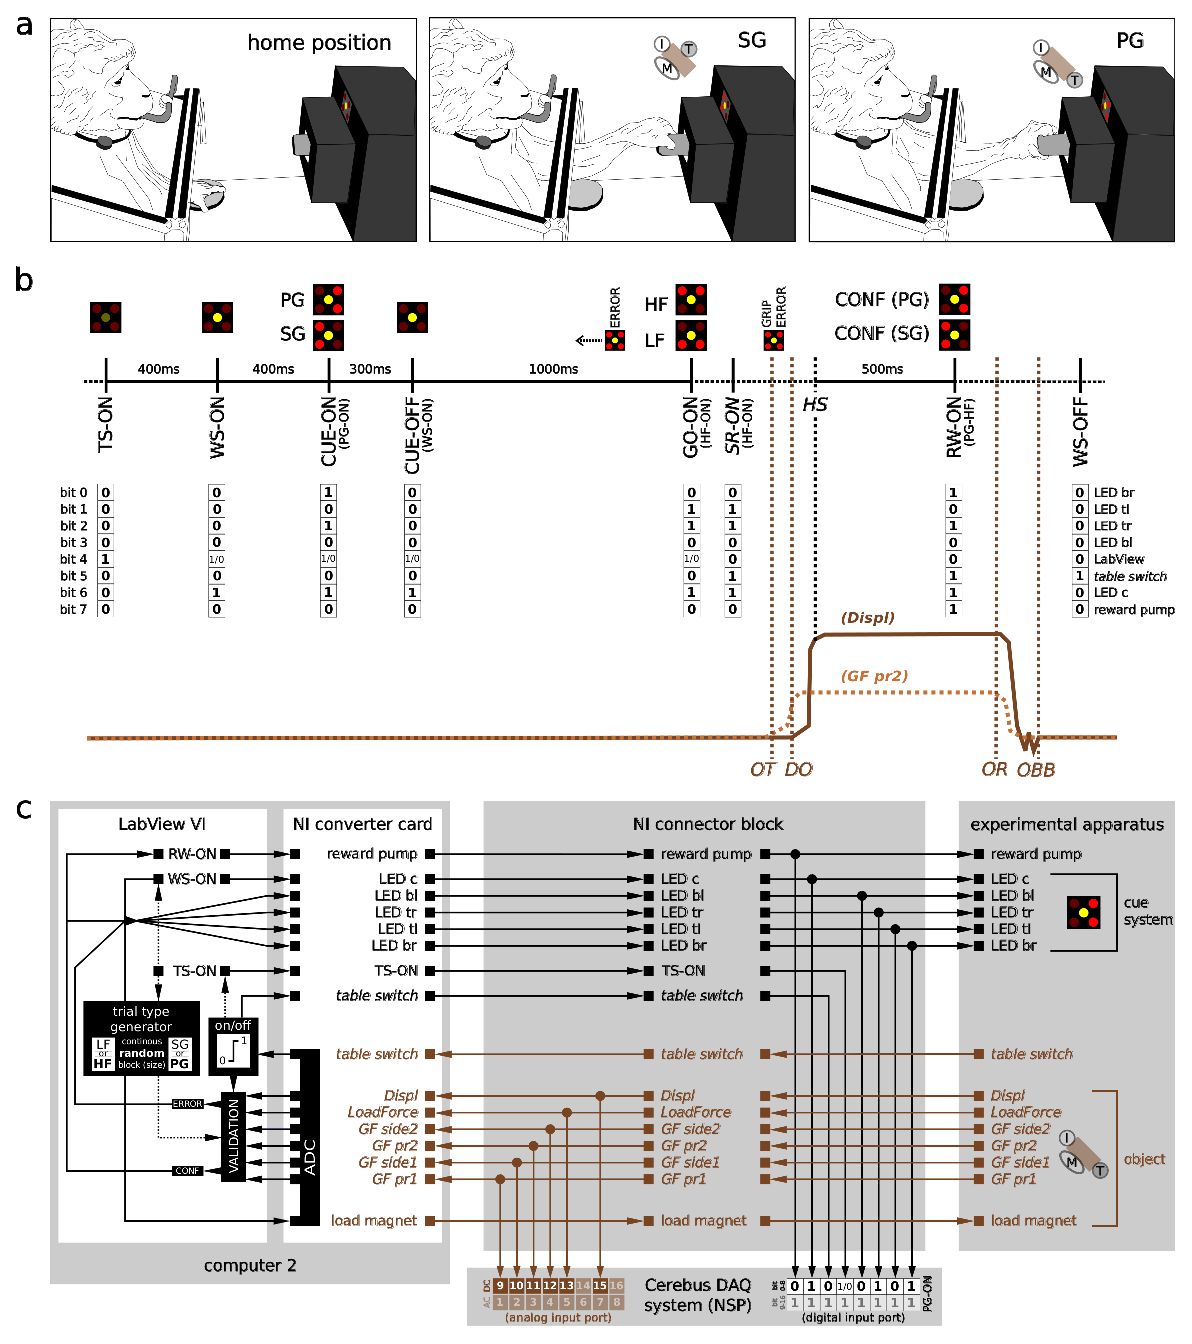
\includegraphics[width=0.8\textwidth]{./figures/scidata_figures/task_trialscheme}
 \caption[Overview of the experimental apparatus and behavioral control system.]{Overview of the experimental apparatus and behavioral control system. (a) Sketches of the experimental apparatus and the monkey performing the reach-to-grasp task. Left: monkey in its home position with the working hand on the table switch. Middle and right: monkey grasping the object with a side grip (SG) and a precision grip (PG), respectively. Insets of middle and right sketch show the actual position of the index finger (I), the thumb (T), and the middle finger (M) on the object (brown cube) 11 . (b) Trial scheme of an example trial with
the respective visual cues (different illumination combinations of the 5 LEDs illustrated on top) shown to the monkey at its respective times. The behavioral events are marked along the time axis (see main text for abbreviations). \code{Event}s with black font mark digitally recorded events, whereas events with brown font indicate events (object touch OT, object release OR, displacement onset DO, and object back to baseline OBB) which were extracted offline from baseline deviations of the analog signals of the object’s sensors. Additionally, we indicate by italic fonts events which were generated by the monkey, while all other events are produced by LabView. The 8-bit binary code for the digital event signals sent from LabView VI to the NSP at the respective times is shown below the time axis. Example traces for the analog signals of the HE sensor (Displ; dark solid line) and one of the 4 FSR sensors located at the object’s surface (GF pr2, light dotted line) used to monitor the monkeys behavior and extract
OT, OR, DO, and OBB are shown at the bottom. (c) Outline of the devices and their wiring controlling the behavior. All analog signal streams are colored in brown, whereas all digital signal streams are colored in black.}
\label{fig:task_trialscheme}
\end{figure}

As already mentioned, the object was equipped with six sensors which monitored the monkey's reach-to-grasp behavior. Four force sensitive resistance sensors (FSR sensors) on the object surface provided continuous measurement of the grip forces applied on the object sides by the index and middle finger, as well as the thumb. The different activation patterns of these four FSR sensors, in particular the different placement of the thumb (see \cref{fig:task_trialscheme} a), were used to detect online if the correct grip type was performed. An additional FSR sensor was installed between the object and its counterweight. This FSR sensor was used to measure the horizontally applied force needed to oppose the corresponding object load. Due to the low, but still existing friction of the object moving inside the horizontal shuttle, the measured force signal of this sensor is not perfectly proportional to the horizontal force needed to lift the opposed object load, but sufficient to distinguish between LF and HF settings (cf., example in bottom right panel of \cref{fig:overview_data_l_1} and \cref{fig:overview_data_n_1}). The horizontal displacement of the object over a maximal distance of 15mm was measured by a hall-effect (HE) sensor. All sensors of the object are summarized in \cref{tab:overview_sensors}. The visual cue system, composed of a square of five LEDs (size 10 x 10 mm), was located just above the target object and used to instruct the monkey about the requested behavior. While the central yellow LED was used to warn the monkey that a trial had started, the four red corner LEDs were used to code separately the grip and the force type for the requested trial type of each trial. In this context the illumination of the two left, the two right, the two bottom, or the two top LEDs coded for SG, PG, LF, or HF, respectively (see \cref{fig:task_trialscheme} b for illustration). The reward system consisted of a bucket filled with apple sauce and equipped with a feeding tube and a pump allowing to deliver on demand the reward (few drops of the apple sauce) to the monkey (\cref{fig:task_trialscheme} a).

\begin{table}[]
\footnotesize
\centering
\begin{tabular}{llllll}
\hline
sensor & channel ID & label     & located at       & activated by          & used to identify  \\ \hline
FSR 1  & 137        & GF pr1    & object’s top     & index finger’s touch  & PG type           \\ 
FSR 2  & 138        & GF side1  & object’s left    & middle finger’s touch & SG type           \\ 
FSR 3  & 139        & GF pr2    & object’s bottom  & thumb touch           & PG type           \\ 
FSR 4  & 140        & GF side2  & object’s right   & thumb touch           & SG type           \\ 
FSR 5  & 141        & LoadForce & object’s spring  & object loading        & pulling force     \\ 
HE     & 143        & Displ     & object's shuttle & object displacement   & object’s position \\ \hline
\end{tabular}
 \caption[Overview of six objects sensors to monitor and control the monkey's behavior]{Overview of the six object sensors used to monitor and control the monkey's behavior. The first four force sensitive resistance (FSR) sensors are used to monitor the applied grip type. They are located on the surface of each object side and are activated by the touch of the corresponding monkey's finger. The fifth FSR is located at the spring counterbalancing the pull resistance of the object and is used to measure the pulling force applied by the monkey. The hall-effect sensor (HE) is located along the low-friction shuttle of the object and used to measure the position of the object. The signals of all sensors are saved in the ns2 with the stated channel ID and label (cf. \cref{fig:cerebus_system}).}
 \label{tab:overview_sensors}
\end{table}

\subsection{Behavioral control system}
\label{sec:behavioral_control_system}

The core of the behavioral control system is a custom-made Virtual Instrument (VI) in LabView that controls the digital event sequence and the requested behavior of each trial in a recording. A digital event reflects hereby the activation or deactivation of a physical device of the experimental apparatus. In this context, the LabView VI is responsible to activate and deactivate the LEDs of the visual cue system, the reward pump, and the electromagnet. The latter is not controlled by a digital event, but by an analog square signal that switches the magnet on or off. To control the requested behavior, the LabView VI monitors the monkey's manipulation of the table switch and the target object. The table switch as well as all sensors of the target object produce continuous analog signals that are digitized by the NI converter card and fed into the LabView VI of the setup computer (see \cref{fig:scidata_setup_overview} computer 2). The square signal of the table switch is then online reinterpreted as digital activation or deactivation event. \cref{fig:task_trialscheme} c displays a schematic diagram on how the physical devices of the experimental apparatus are connected to the setup computer and controlled and monitored by the LabView VI. We will now describe a typical execution of the LabView VI during a recording session in more detail. 

\begin{figure}
 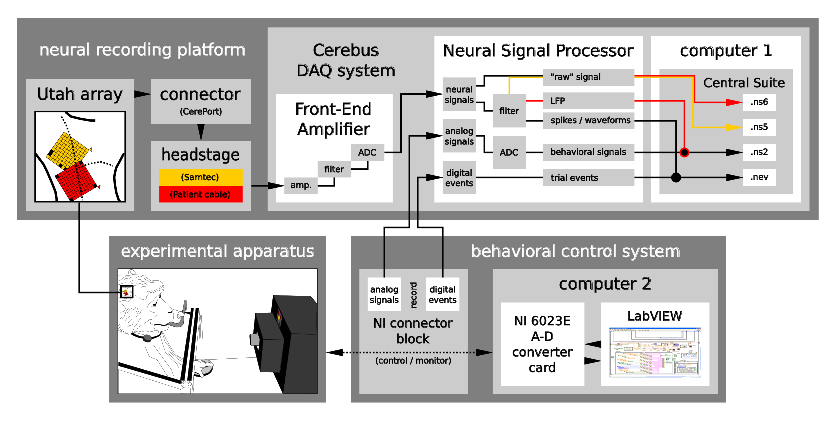
\includegraphics[width=\textwidth]{./figures/scidata_figures/setup_overview}
 \caption[Overview of the setup]{Overview of the setup. The setup consisted of three main parts: the neural recording platform, the experimental apparatus, and the behavioral control system. The neural recording platform (top) was composed of the implanted Utah array with its corresponding connector (CerePort), a headstage (Samtec or Patient cable), and the Cerebus data acquisition (DAQ) system (i.e. the Front-End Amplifier, Neural Signal Processor (NSP), and the Cerebus control software, Central Suite, installed on the setup computer 1). The experimental apparatus (bottom left) consisted of the physical devices which the monkeys had to interact with (i.e., the visual cue panel (square with 5 LEDs), the target object, the table switch, and the reward system). The behavioral control system (bottom right) was built from hard- and software of National Instruments (NI, National Instruments Corporation, Austin, Texas, USA). It was composed of a NI connector block which was linked via a NI 6023E A-D converter card to setup computer 2 on which the NI system design software, LabView, was running. To record the behavioral data the behavioral control system was interlinked with the neuronal recording platform via the NSP and the NI connector block. All three parts are separately described in more detail in the main text, as well as Figures 2 and 4. Setup differences between the two monkeys are indicated in yellow and red for monkeys L and N, respectively.}
 \label{fig:scidata_setup_overview}
\end{figure}

The possible trial types were set to SG-LF, SG-HF, PG-LF, and PG-HF, alternating with equal probability randomly in sequence between trials. Once the settings of the overall task were defined, the LabView VI was started to repetitively run and control the event sequence and behavior for each trial during the recording session. 

Each single trial was run and controlled as follows: 

The LabView VI only started a trial when the monkey deactivated the table switch by pressing and holding it down (home position, \cref{fig:task_trialscheme} a, left). This required not much muscle activity, but simply the weight of the monkey's hand on top of the smooth-running switch. If the table switch was deactivated, the LabView VI internally initiated a trial with a short time delay (TS-ON). In parallel, the program picked randomly one of the possible trial types (e.g., SG-HF) and activated or deactivated the electromagnet accordingly to fit the chosen load force of the object (e.g., activated for HF). To inform (or warn) the monkey that a new trial has started, the central LED was illuminated 400ms after the trial was initiated by the program (WS-ON). Four hundred ms after WS-ON the grip type was revealed to the monkey by illuminating the corresponding corner LEDs of the chosen trial type (CUE-ON, e.g., left LEDs for SG-ON). The LEDs of this first cue were turned off again after 300ms (CUE-OFF). The CUE-OFF was followed by a 1000ms preparatory delay at the end of which the monkey was informed about the upcoming force type by again illuminating the corresponding corner LEDs of the chosen trial type (GO-ON, e.g., top LEDs for HF-ON). This second cue also served as a GO signal for the monkey to initiate the movement which was registered by the activation of the table switch (SR-ON) when the monkey released it after a variable reaction time (RT). The execution of the movement was composed of reaching, grasping, pulling and holding the object in the position window for 500ms. The LabView VI controlled the movement execution online by checking the used grip type, the object displacement and the hold time. For checking the grip type, the grasp of the object was registered by small deflections of the FSR surface sensor signals caused by the monkey's fingers. A FSR sensor was registered as activated if the deflection surpassed a predefined threshold. The pattern of activated FSR sensors was then used by the LabView VI to control if the monkey performed the requested grip type. This meant, in particular, to check for SG and PG, if the FSR sensor on the right (GF side2), or on the bottom (GF pr2) of the object was activated by the monkey's thumb, respectively (see \cref{fig:task_trialscheme} a, middle and right). The other 2 sensors that measured force from the index and middle fingers for the 2 grip types (GF side1, and GF pr1) were not controlled online. If the correct grip was detected, the grip cue was illuminated again as a positive feedback. To check the object displacement, the LabView VI measured if the deflection of the HE sensor signal of the object was within the two defined position thresholds (4 and 14mm). The time point at which the displacement signal surpassed the lower threshold was used by the LabView VI to define the estimated start of the holding period (HS) online. If the object remained within the position window for 500ms after the HS was set, LabView activated the reward pump which provided the monkey with a drop of apple sauce as reward for a successful trial. The time until the reward pump was deactivated again by LabView was proportional to the duration of the object hold in the position window, with a maximum duration and with this a maximum amount of reward for a 500ms holding period. With this mechanism, both monkeys rapidly learned to hold the object at least 500ms in nearly all trials. In parallel to the deactivation of the reward pump, LabView turned off all LEDs to indicate that the running trial ended (WS-OFF). The monkey was allowed to release the object at its own pace as soon as it received the reward. A new trial sequence was started by LabView (TS-ON) as soon as the monkey returned to the home position (new deactivation of the table switch).

An abort of the described trial sequence by LabView (error trial) was triggered by the following three scenarios: (i) the monkey released the table switch before the GO cue, (ii) the wrong grip type was registered, and (iii) the object was not pulled and held long enough in the position window. In case one of these scenarios were registered by LabView the trial was aborted. For monkey L, the LabView VI provided additionally a negative feedback when aborting a trial by flickering all LEDs three times. 

As displayed in \cref{fig:task_trialscheme} c. the behavioral control system was connected to the NSP of the Cerebus DAQ system to store the trial event sequence and the monkey's behavior of each trial in a recording along with the neural data registered by the neural recording platform. For this, the analog signals of the sensors of the target object were copied from the NI connector block to the analog input port of the Cerebus System NSP via DC coupled BNC cables and connectors. In the NSP they were digitized with a 16-bit resolution at 0.15 mV/bit and a sampling rate of 1kHz and saved in the ns2 file under the channel ids listed in \cref{tab:overview_sensors}. All digital or digitized events that register the activation and deactivation of the table switch, the LEDs of the cue system, and the reward pump, as well as the internally generated digital trial start event (TS-ON) were coded as a 8-bit binary signal (see \cref{tab:bit_translation}) and transferred via the NI connector block to a 16-bit DB-37 input port of the NSP where they occupy the first 8 digits (remaining digits are set to 1). In the NSP the now 16-bit binary signal of each event was stored in its decimal representation and with its corresponding time point in the nev file (see \cref{tab:bit_translation} and \cref{fig:cerebus_system}).


\subsection{Neural recording platform}
\label{sec:neural_recording_platform}
The recording of the neural signals was performed using a neural recording platform with components produced by Blackrock Microsystems (Salt Lake City, UT, USA, www.blackrockmicro.com). The platform consisted of the multi-electrode Utah array, a headstage, and a Cerebus data acquisition (DAQ) system. The latter is composed of a Front-End Amplifier, a real-time Neural Signal Processor (NSP) and the control software, Central Suite (version 4.15.0 and 6.03.01 for L and N, respectively), running on Windows XP for L, and Windows 7 for N on the setup computer 1 (see Fig. \cref{fig:cerebus_system}). The Cerebus DAQ system was also connected to the behavioral control system via the NI connector block to save the analog behavioral data and digital trial event signals that were described in the previous section in parallel with the neural signals. All data were transmitted from the NSP via an ethernet cable to be saved first locally on the setup computer 1. After a recording day, all recordings were transferred to a data server. In the following, we will describe the function of the different components of the neural recording platform in more detail.

The implant location of the Utah array, as well as the electrode configuration of the array of each monkey was described previously (see \cref{fig:implant_locations}). The electrode identification numbers (IDs) are determined by how the electrodes of the array are wired and connected to the Cerebus Front-End Amplifier. See \cref{sec:channel_ids} for details.

The analog Blackrock headstage with unity gain (Samtec for monkey L, and Patient Cable for monkey N) was used to reduce the environmental noise. Overall, the reduction of the noise was better with the Patient Cable than with the Samtec headstage.

In the Front-End Amplifier, each of the 96 neural signals was differentially amplified with respect to the reference input of its corresponding connector bank (gain 5000) and filtered with a 1st-order 0.3Hz high pass filter (full-bandwidth mode) and a 3rd-order 7.5kHz Butterworth low pass filter. After that, the band-pass filtered neuronal signals were digitized with a 16-bit resolution at 0.25V/bit and a sampling rate of 30kHz, in the following called “raw signal”. The digitized signals were converted into a single multiplexed optical output and transmitted via a fiber-optic data link to the NSP. In the NSP the raw signals were saved in a ns5-file for monkey L and in a ns6-file for monkey N. The file format depended on the firmware and software version of the Cerebus DAQ system. In addition to the neural signals, the NSP received the analog behavioral signal recorded by the behavioral control system via the analog input port. These behavioral signals were digitized and saved with a sampling rate of 1kHz in a ns2-file. For monkey N, the ns2-file also contained a filtered and downsampled version of the raw signals, in the following called “LFP data”. To extract the LFP data, a copy of the raw data was online digitally low-pass filtered at 250Hz (Butterworth, 4th order), and downsampled to 1kHz within the NSP.

The NSP performed also an online spike waveform detection and classification controlled via the Central Suite software. The sorted spikes were used for a first online inspection of the data as well as for selecting and saving the spike waveforms for offline sorting. For this purpose the neuronal raw signals were for monkey L online high-pass filtered at 250 Hz (Butterworth, 4th order) and for monkey N band-pass filtered between 250Hz and 5kHz (Butterworth, 2nd order). Afterwards, the waveforms were detected by threshold crossing (manually set). These waveforms were then sorted by requesting the signal from identified neurons to follow through up to five hoops set by the user (all individually for each channel). To get an overview of the quality of the data during the recordings, the sorted waveforms were displayed in the online classification window provided by Central Suite.

The thresholds (one for each channel) for the spike waveform detection were not modified during a session and were saved in the nev-file for each session along with all other settings (e.g. filter setting etc) and configurations of Central Suite. The data and corresponding settings of Central Suite can also be inspected offline using the Blackrock software CentralPlay even in the absence of the Blackrock hardware system. Each time the high-pass filtered signal passed the threshold, a snippet of 1.6ms (48 samples) for monkey L and 1.3ms (38 samples) for monkey N was cut and saved as potential spike waveform. The snippet was cut with 10 sample points before threshold crossing and 38 or 28 points after for monkey L or N, respectively. Waveforms identified as potential single units (online sorted spikes) were labeled with IDs from 1 to 16. Unsorted waveforms were labeled with ID 0. These potential spike waveforms were saved together with their respective time stamps in the nev-file. Due to the high number of electrodes, online spike-sorting was moderately reliable. We therefore decided to re-sort spiking activity offline on each channel using the Plexon Offline Spike Sorter (Plexon Inc, Dallas, Texas, USA, version 3.3, for details see \cref{sec:data_preprocessing}). Results of offline sorting were saved in a copy of the original nev-file with an updated file name. 

All data files (nev, ns5/6, ccf) were saved on disk and backed-up on a data server at the end of the recording sessions. The information collected here are partly taken from \citep{Riehle_2013, Zehl_2016}.


\subsection{Origin of the channel IDs}
\label{sec:channel_ids}

The neuronal signal inputs to the Front-End Amplifier were grouped into four banks (A-D or 0-3) from which only the first 3 were used. Each bank consists of a male header with 34 pins of which 32 were the neuronal signal input channels. The other two channels served as reference and ground, respectively. In Central Suite, the identification (ID) number of each electrode of the array is defined by the position on the input bank and pin of the Cerebus Front-End Amplifier. For this Central Suite multiplies the bank ID (0, 1, 2, or 3) with the number of pins for neural signal input channels (32) and adds the ID of the pin the electrode is connected to (cf. ID conversion in \cref{fig:cerebus_system}). The electrode wiring of the Utah array is, though, not coordinated to the input banks of the Front-End Amplifer which leads to spatially unordered electrode IDs. Nevertheless, Utah arrays are fabricated usually in the same way where the corner electrodes are unconnected leading to a default (unordered) electrode ID configuration (cf. electrode configuration of monkey N in \cref{fig:implant_locations}). If in the fabrication process one of the corner electrodes was registered to be of significantly higher quality than any other electrodes of the grid, the corner electrode was connected instead and thereby changed the corresponding electrode configuration (cf. electrode configuration of monkey L in \cref{fig:implant_locations}). This led to the different ID sequences of the arrays for monkey L and N (see \cref{fig:implant_locations}). To facilitate the comparison of results between arrays with different electrode configurations, we assigned new IDs that reflect the spatial organization of the array. For this we used as reference the lower left corner electrode, when the connected wire bundle is showing to the right. These fabrication-independent, connector-aligned IDs increase linearly from bottom left to top right, line by line. They are also shown in \cref{fig:implant_locations} d as gray numbers in the array sketch, which thereby provides the mapping of the Blackrock IDs to the connector-aligned IDs. 

\begin{figure}
 \centering
 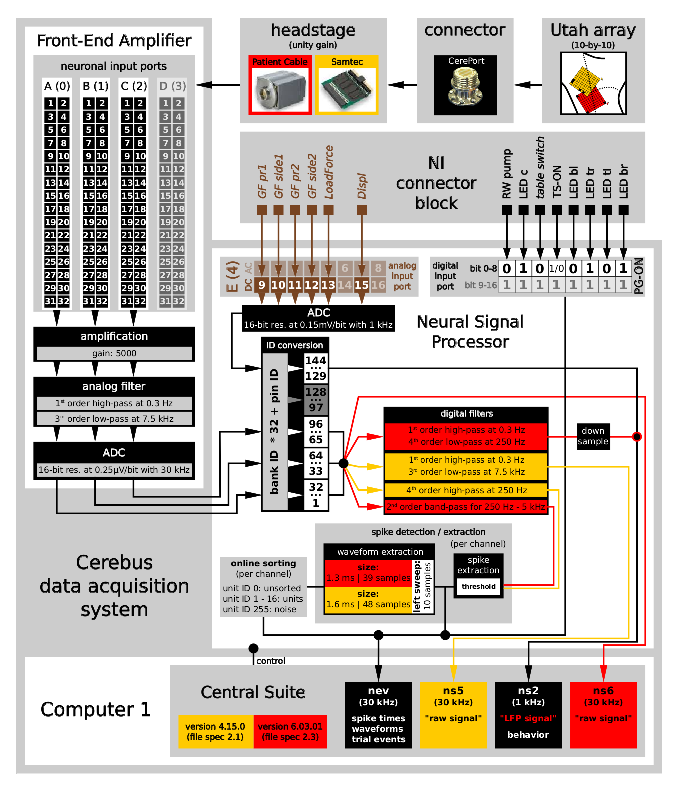
\includegraphics[width=0.7\textwidth]{./figures/scidata_figures/cerebus_system}
 \caption[Sketch of the components related to the recording of the neuronal signals]{Sketch of the components related to the recording of the neuronal signals. Data were recorded
using a Utah array, which was linked via its connector (CerePort) to a headstage (Samtec or Patient Cable) with a unity gain. From there the neural signals were transferred to the Cerebus Front-End Amplifier, where they were amplified, filtered and digitized. The digitized signals were converted into a single multiplex optical output and sent via a fiber-optic data link to the Neural Signal Processor (NSP), which is controlled by the Cerebus control software (Central Suite). Within the NSP the time points and waveforms of potential spikes were extracted online from a correspondingly processed copy of the neural signals and saved in the nev file. Simultaneously, the continuous raw signals (sampled at 30 kHz) were saved in the ns5 (for monkey L) or ns6 file (for monkey N). In parallel to the neural signals the NSP received also the digital trial events produced by the LabView VI, and the analog signals of the object’s sensors via the NI connector block of the behavioral control system. While the digital trial events were saved along with the extracted potential spikes in the nev file,
the analog signals of the sensors were digitized and saved in the ns2 file. For monkey N, a filtered and downsampled version of the neural signals (0.3–250 Hz at 1 kHz) was also saved in the ns2 file. Components and settings specific to monkey L and N are indicated by yellow and red, respectively.}
\label{fig:cerebus_system}
\end{figure}

A visual summary of the available data is given in \cref{fig:overview_data_l_1} and \cref{fig:overview_data_l_2}  for monkey L, and \cref{fig:overview_data_n_1} and \cref{fig:overview_data_n_2} for monkey N. The first of these figures shows the sequence of trials as well as selected raw recorded time series, spike trains, unit wave forms, and behavioral signals for one particular trial. The second of these figures contrasts parallel neuronal data across channels in a specific trial with neuronal data across trials in a specific channel.


\section{Data preprocessing}
\label{sec:data_preprocessing}

After the recordings, a number of preprocessing steps (pre in the sense of before the actual upcoming data analysis, but being the post-processing after the recording) were performed as described below. This includes (i) the translation of the digital events from their binary codes set by the DAQ system to a human-readable format putting the events in context of the expected executed trial event sequence, (ii) the offline detection of behavioral trial events and object load force from the analog signals recorded by the sensors of the target object, and (iii) the offline spike sorting.

\subsection{Translation of digital events to trial events }

\cref{tab:bit_translation} lists the 8-bit combinations that were sent by LabView to the Experimental Apparatus to control the behavior. Following a binary to decimal conversion, they were saved as event codes (\cref{tab:bit_translation}) during the experiment along with their time stamps in the .nev file. In the first preprocessing step, these event codes were translated to a human-readable format and put into context of an expected trial event sequence. The validation against the latter was used to identify incomplete, correct and error trials. Error trials were further differentiated into error types (e.g., grip error). This digital event translation and interpretation (cf. \cref{tab:bit_translation}) performed automatically within the reach-to-grasp loading routine. 

Translation table of the 8 bits to the event codes and their behavioral meaning (labels). The 8 bits (see \cref{tab:bit_translation} for their meaning) were sent from LabView to NSP during the trial sequence (Fig. \cref{fig:task_trialscheme}). The event codes are the decimal version of the bit sequence assuming another byte with all bits set to 1 in front. The event codes are found in the .nev files with a time stamp and indicate the occurrence of a stimulus / behavioral event as indicated in the center column ('label'). Due to different versions of the LabView control program for monkey L and N (see text for details) the event codes for the same label may be different for the two monkeys. Also some event codes do not have a concrete meaning (miscellaneous) and occur sporadically in the .nev file due to a mistake in the sampling of the digital events - they have to be ignored. In the table the event codes are sorted in sequential order from top to bottom with respect to the task, i.e. their order corresponds to the sequence found in the .nev file in an successful trial. 

\subsection{Preprocessing of behavioral analog signals}

Some behavioral events such as the monkey touching the object or the onset of the object displacement by the monkey were controlled during the experiment, but their online-detected timing was approximate and not saved (see details in section \cref{sec:behavioral_control_system}). However, these events can be relevant for data analysis and they were thus computed offline from the analog signals of the four FSR sensors measuring the monkey's grip and the HE sensor measuring the object displacement. We implemented a custom-made Matlab \code{Event}-Detection toolbox to detect 8 specific events: the precise timing of object touch (OT) and object release (OR) from the force traces as well as the timing of displacement onset (DO) and object back to baseline (OBB) from the displacement trace, and finally the onset and offset of the plateau phase in the force and displacement traces. The plateau phase of the displacement signal indicates the timing and stability of the holding period, and its onset is used to calculate offline the hold start (HS) signal. The toolbox performed an automatic detection of these events and their timing was first approximated by threshold crossing and then fine-tuned by back-comparison of the traces with baseline level from the point of threshold crossing. Since the automatic detection was prone to errors, the trials were visually inspected one by one and the timing of the automatically detected events were manually corrected if they did not match the event times as visually identified. In addition, a Matlab script was used to inspect the load force traces in each trial to control if the actual object load corresponded to the programmed object load. This procedure ensured that the electro-magnet controlling the object load was properly activated throughout the recording session. 

\subsection{Offline spike sorting}
\label{sec:offline_spike_sorting}
The spike waveforms which were extracted and saved (in the nev file) during the recording were offline sorted using the Plexon Offline Sorter (version 3.3.3). To keep the variability in the half-manual spike sorting at a minimum, all sortings were performed by the same person (A. Riehle). The spike sorting started with loading the complete nev file of a session into the Plexon Offline Sorter. The spike sorting was performed on a duplicate of the data file to keep the original data intact. We started by joining all different waveforms extracted online from each channel separately back again into one pool and initially marked as “unsorted waveforms” in the Plexon Offline Sorter. Thereby, we ignored the result of the preliminary online waveform sorting (units 0-16 in the nev file) that was performed during the recording via Central Suite software, which served solely to extract waveforms and gain an overview of the quality of the spiking activity. For the invalidation of cross-channel artifacts (e.g., chewing artifacts) all waveforms that occurred simultaneously on a defined percentage of channels (70\%) were marked as “invalidated waveforms” in Plexon Offline Sorter. Such artifacts occurred only in the recording session of monkey L. Furthermore, a waveform rejection was performed. Thereby all waveforms of abnormally large amplitude and/or atypical shape on a channel were manually marked as “invalidated waveforms” in Plexon Offline Sorter.

The actual spike sorting was then performed on the remaining unsorted waveforms (i.e., those not marked as invalidated waveforms) individually for each channel. We used different algorithms to split these waveforms into clusters in a 2- or 3-dimensional principal component (PC) space. The dimensionality of the PC space was chosen according to the best separation. The main algorithms used were K-Means(-Scan) and Valley Seeking (chosen according to the best separation). We used a fixed threshold for outliers (a parameter to be determined in the Plexon Offline Sorter) between 1.8 (K-Means) and 2 (Valley Seeking) to get comparable sorting results. The spikes of the sorted clusters were then controlled using the inter-spike interval (ISI) distributions and the auto- and cross-correlation plots. Units were ordered manually from best to worst (assigning increasing unit IDs 1-16 in the Plexon Offline Sorter) by considering the amplitude of the waveform (the higher the better), the outcomes of the ISI analysis (no or low number of spikes with an ISI smaller than 2 ms), the correlation histograms, and identifiable cluster shapes. Waveforms in the cluster with the highest unit ID (worst) on a given channel may contain multi-unit activity. Clusters with unacceptable outcomes (completely or partly overlapping waveforms), including those with only a few spikes, left assigned as “unsorted waveforms” in Plexon Offline Sorter. This offline spike sorted nev file was saved under the file name of the original nev file with an added two-digit numeric postfix (e.g. -01). In this file, unit ID 255 contains invalidated waveforms, unit ID 0 contains the unsorted waveforms (that may enter a further cluster analysis for spike sorting), and unit IDs 1-16 contain the time stamps and waveforms of the sorted single- or multi-units (as in the Plexon Offline Sorter). Unit IDs that are considered to represent multi-unit activity are documented in the metadata. The nev file with the sorted units can be loaded again into the Plexon Offline Sorter to visualize all the sorted spikes and rework the spike sorting.

\begin{table}
\centering
\begin{tabular}{cccccc}
\hline 
\multirow{2}{*}{\textbf{monkey}} & \multirow{2}{*}{\textbf{sorting ID}} & \multirow{2}{*}{\textbf{\# SUA}} & \multirow{2}{*}{\textbf{\# MUA}} & \multicolumn{2}{c}{\textbf{\# electrodes with}}\tabularnewline
% \cline{5-6} 
 &  &  &  & \textbf{SUA} & \textbf{SUA or MUA}\tabularnewline
\hline 
\hline 
\textbf{L} & {*}-02 & 93 & 49 & 65 & 86\tabularnewline
\textbf{N} & {*}-03 & 156 & 19 & 78 & 89\tabularnewline
\hline 
\end{tabular}

\caption[Overview of offline sorted single and multi unit activity (SUA and MUA)]{Overview of offline sorted single and multi unit activity (SUA and MUA). For the recording of monkey L it was possible to sort out 93 SUAs and 28 MUAs distributed over 65 of the 96 electrodes of the Utah array, with 21 additional electrodes with further MUA recordings. For the recording of monkey N it was possible to sort out 156 SUAs and 8 MUAs distributed over 78 of the
96 electrodes of the Utah array, with 11 additional electrodes with further MUA recordings. For details on the offline spike sorting see \cref{sec:offline_spike_sorting}.}
\label{tab:datafiles_unitactivity}
\end{table}

\subsection{Code availability}
\label{sec:code_availability}

All available code required to access the data as described in \cref{sec:usage} is stored along with the datasets. The provided code includes, in particular: (i) a snapshot of the Python \software{Neo}  package (see also \cref{sec:neo}), (ii) a snapshot of the Python \software{odML} package (see also \cref{sec:odml}), (iii) the custom-written ReachGraspIO extending the \software{Neo} package, (iv) the example script shown and described in \cref{sec:usage}, (v) the code shown and described in \cref{sec:usage} demonstrating how to access the data in \software{Matlab}.

In addition to these frozen versions of the code, we recommend to use updated versions of the code to benefit from future enhancements, bug fixes and increased compatibility with future Python releases or novel applications that rely on recent versions of \software{Neo} and/or \software{odML}. Complete link collections to the two libraries can be found online\footnote{\software{Neo}, \url{http://neuralensemble.org/neo/}},\footnote{\software{odML}, \url{ and http://www.g-node.org/projects/odml}}. Importantly, both projects are hosted and version-controlled via Github\footnote{\software{Neo}, \url{https://github.com/NeuralEnsemble/python-neo}},\footnote{\software{odML}, \url{https://github.com/G-Node/python-odml}}.

\section{Data records}

All data and metadata are publicly available via the data portal of the German Neuroinformatics Node (G-Node) of the International Neuroinformatics Coordination Facility (INCF), called GNData\footnote{GNData, \url{http://g-node.github.io/g-node-portal/}}. \cref{tab:scidata_data_overview} provides an overview of the name, size, and content of all files for each published dataset of monkey L and N. The datasets of both monkeys consist of four parts: (i) the primary data are provided as the original data files obtained from the Central Suite software stored in the data format specified by the manufacturer (in particular, nev, ns5 and ns6 format) of the neural recording platform, Blackrock Microsystems; (ii) an offline sorted version of the neural spike data (cf. \cref{sec:offline_spike_sorting}) is provided in a second nev file; (iii) metadata are provided as one file per dataset in the \software{odML} format \citep{Grewe_2011, Zehl_2016}; and (iv) a mat file is provided containing the continuous neural raw data together with the offline sorted spike data, both annotated with the corresponding metadata.

\begin{figure}
 \centering
 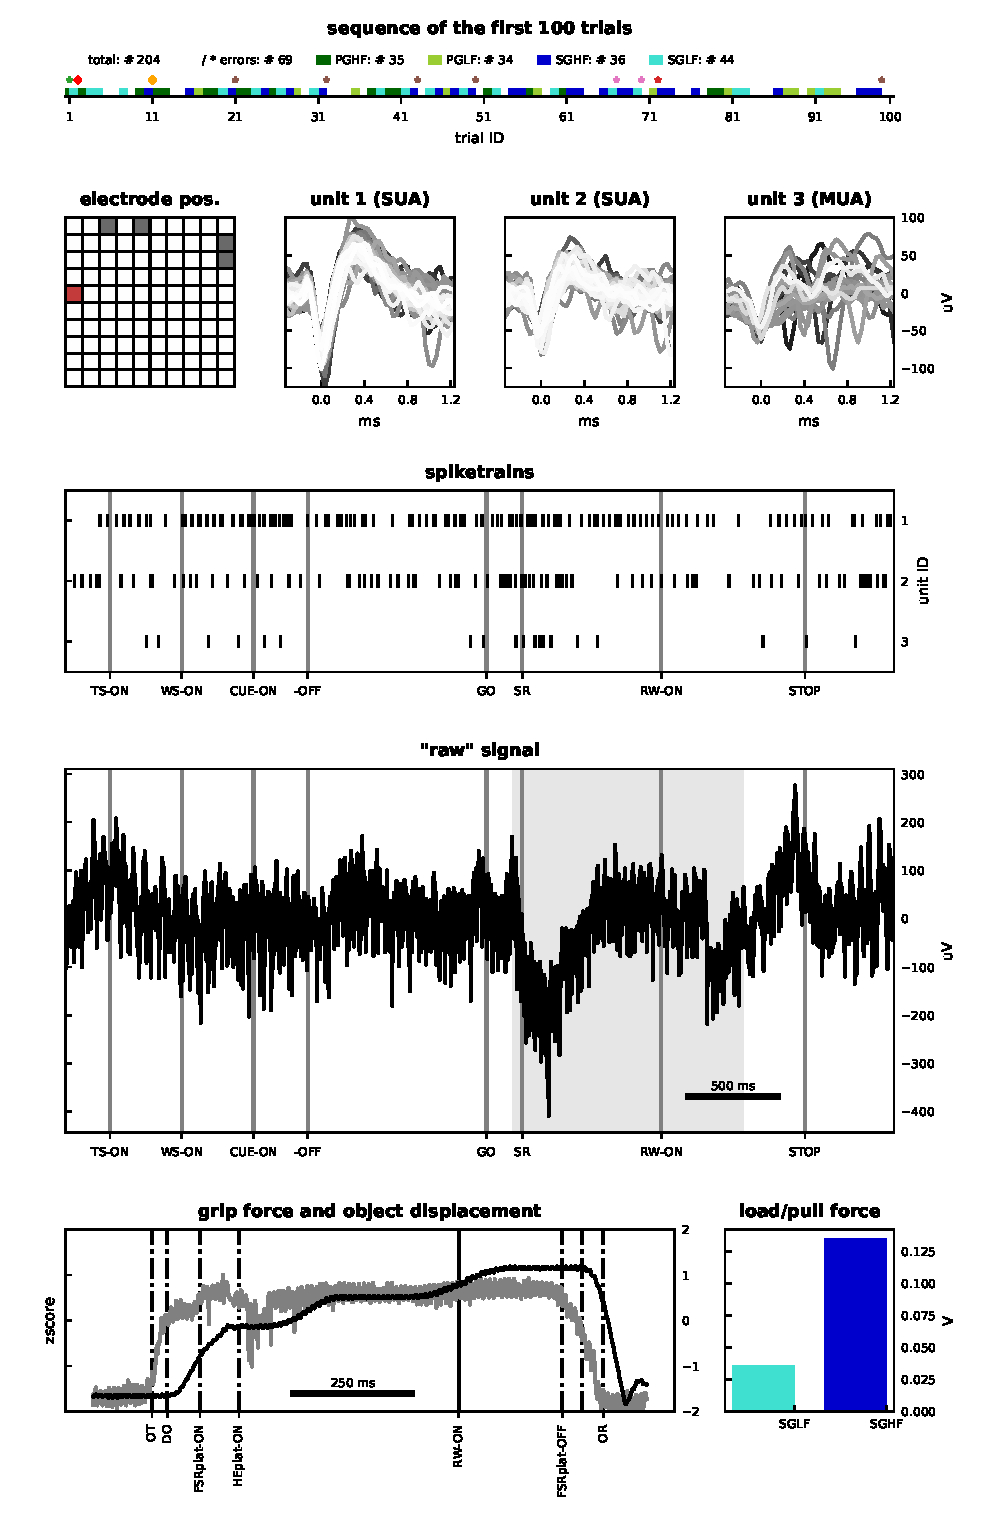
\includegraphics[width=0.8\textwidth]{./figures/scidata_figures/data_overview_1_L}
 \caption[Overview of data types contained in l101210-001]{Overview of data types contained in l101210-001. The figure displays the different data types contained in the selected dataset of monkey L. Top panel: sequence of the first 100 trials (for trial types and errors see color in legend) and the total number of trials (see \# for correct, error, trial types in legend); the red diamond marks the selected trial (trial ID: 2) for panels below; the orange diamond marks an additional trial selected to demonstrate load/pull force differences between the averaged load force signals in the bottom right panel. Asterisks indicate error trials (black asterisks: grip errors). Second row, left panel: position of selected electrode (in red) for the data plots (electrode ID: 71). Second row, remaining panels: waveforms of three units from the selected electrode. Third row: spike trains of displayed units for the selected trial. Forth row: raw signal for the selected trial; gray shaded area marks the time window corresponding to the bottom left panel. Bottom left panel: grip force (gray) and object displacement (black) signals for the selected trial. Bottom right panel: averaged load/pull force signals for the duration of the plateau of the grip force signal for the selected LF and HF trial. Important trial events are indicated as vertical lines in the corresponding data plots.}
 \label{fig:overview_data_l_1}
\end{figure}

\begin{figure}
 \centering
 \includegraphics[width=\textwidth]{./figures/scidata_figures/data_overview_2_L}
 \caption[Overview of raw signal and spike data of monkey L (l101210-001)]{Overview of raw signal and spike data of monkey L (l101210-001). Left panels: Raw signal (top) and spike data of unit IDs 1 on each given electrode (bottom) for a single trial (trial ID: 2) across a selection of electrodes. Right panels: Raw signal (top) and spike data from single unit ID 1 (bottom) across selected correctly performed trials on one electrode (electrode ID: 3). Trial events (TS-ON, WS-ON, CUE-ON, CUE-OFF, GO-ON, and RW-ON) are indicated as colored vertical lines in each plot. Trial types of selected trials in upper right panels are indicated as color (SGHF: dark blue; SGLF: cyan; PGHF: dark green; PGLF: light green)}
 \label{fig:overview_data_l_2}
\end{figure}

\begin{figure}
 \centering
 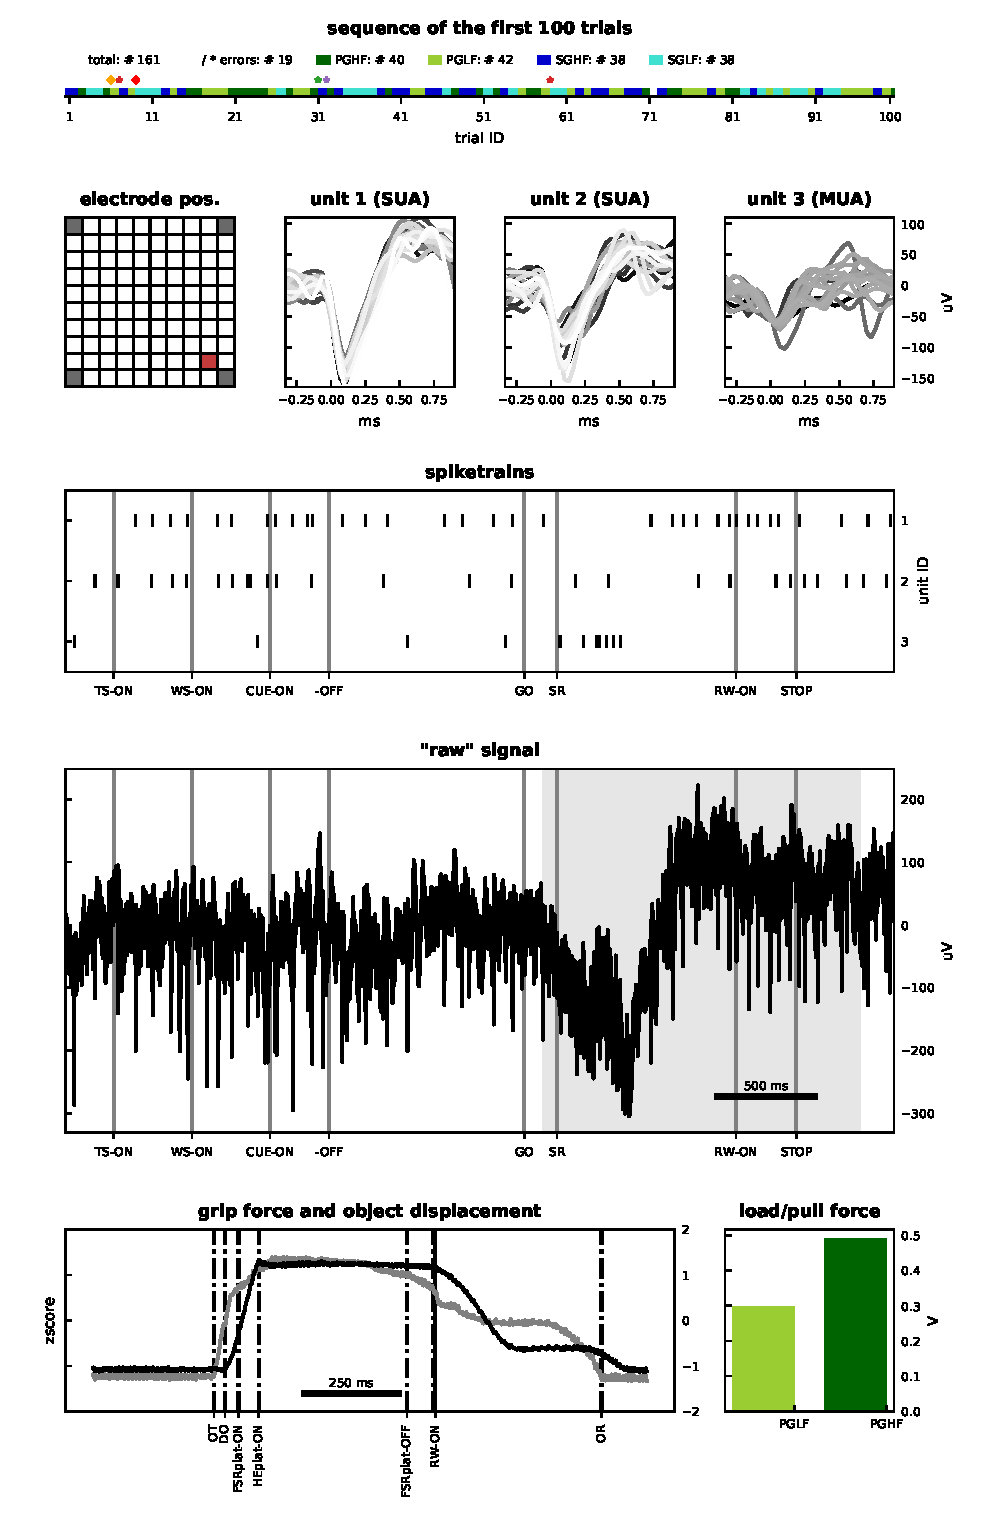
\includegraphics[width=0.8\textwidth]{./figures/scidata_figures/data_overview_1_N}
 \caption[Overview of data types contained in i140703-001]{Overview of data types contained in i140703-001. The figure displays the different data types contained in the selected dataset of monkey N. Top panel: sequence of the first 100 trials (for trial types and errors see color in legend) and the total number of trials (see \# for correct, error, trial types in legend); the red diamond marks the selected trial (trial ID: 9) for panels below; the orange diamond marks an additional trial selected to demonstrate load/pull force differences between the averaged load force signals in the bottom right panel. Asterisks indicate error trials (black asterisks: grip errors). Second row, left panel: position of selected electrode (in red) for the data plots (electrode ID: 63). Second row, remaining panels: waveforms of three units from the selected electrode. Third row: spike trains of displayed units for the selected trial. Forth row panel: raw signal for the selected trial; gray shaded area marks the time window corresponding to the bottom left panel. Bottom left panel: grip force (gray) and object displacement (black) signals for the selected trial. Bottom right panel: averaged load/pull force signals for the duration of the plateau of the grip force signal for the selected LF and HF trial. Important trial events are indicated as vertical lines in the corresponding data plots.}
 \label{fig:overview_data_n_1}
\end{figure}

\begin{figure}
 \centering
 \includegraphics[width=\textwidth]{./figures/scidata_figures/data_overview_2_N}
 \caption[Overview of LFP and spike data of monkey N (i140703-001)]{Overview of LFP and spike data of monkey N (i140703-001). Left panels: LFP data (top) and spike data of unit IDs 1 on each given electrode (bottom) for a single trial (trial ID: 1) across a selection of electrodes. Right panels: LFP data (top) and spike data from single unit ID 1 (bottom) across selected correctly performed trials on one electrode (electrode ID: 1). Trial events (TS-ON, WS-ON,CUE-ON, CUE-OFF, GO-ON, and RW-ON) are indicated as colored vertical lines in each plot. Trial types of selected trials in upper right panels are indicated as color (SGHF: dark blue; SGLF: cyan; PGHF: dark green; PGLF: light green).}
 \label{fig:overview_data_n_2}
\end{figure}


Overview of recording days of the published datasets. For both monkeys, we chose to publish the first dataset (rec*-001) of the recording day. For details on the published datasets see \cref{tab:scidata_data_overview}.

The dataset l101210-001 from monkey L is the first out of 9 recording sessions conducted on Friday, December 10, 2010, while the dataset i140703-001 from monkey N is the first out of only 3 recording sessions conducted on Thursday, July 3, 2014. Both datasets were recorded in the late morning. The following recording day went on for nearly one hour and a half for monkey L, and one hour for monkey N. Although the recording from monkey N lasted with 16:43 min several minutes longer than the recording from monkey L with only 11:49 min, monkey L executed 204 trials, while monkey N only performed 160 trials in total. However, monkey L performed only ~70\% of all trials correctly, whereas monkey N successfully completed ~90\% of all trials during the recording (cf. \cref{tab:scidata_data_overview}). Nonetheless, the high percentage of error trials in monkey L are mainly caused by an too early movement onsets reflecting the eagerness, but also the nervousness of the monkey L's character. In contrast to these error types, monkey L used only 12 times the wrong grip compared to monkey N who performed an incorrect grip type 16 times during the recording. 

Overview of trials performed during the published datasets. Of the stated number of error trials, the monkey L and N used the wrong grip type in 12 and 16 trials, respectively. In the remaining error trials the monkeys initiated the movement too early. Trial types were altered randomly in the recordings which led to slightly different trial numbers for the different trial types.

For both monkeys the trial types alternated randomly between trials leading to slightly different numbers of trials with the same trial type in the each dataset (cf. \cref{tab:scidata_data_overview}). 

The quality of the spiking activity in the datasets of both monkeys was high, which allowed us to perform a relatively robust offline spike sorting with high numbers of single unit activity (SUA) distributed over all electrodes of the array (for details see \cref{tab:datafiles_unitactivity}). For details on how the offline sorting was performed and checked please have a look at \cref{sec:offline_spike_sorting} and \cref{sec:spike_data_quality}. 


\section{Technical validation}
\label{sec:technical_validation}

In addition to the above described preprocessing steps that needed to be performed to gain more content of the raw data, some technical validations of the data also had to be conducted. These technical validations include the correction of the irregular alignment data files of the Cerebus DAQ system and a general quality assessment of the data. In order to validate the quality of the recording, a series of algorithms were applied to the data. On the one hand the quality of the LFP signals was assessed per electrode and per trial by evaluating the variance of the corresponding signal in multiple frequency bands. On the other hand the quality of the offline sorted single units (\cref{sec:offline_spike_sorting}) was determined by a signal-to-noise measure. In addition, noise artifacts occurring simultaneously in the recorded spiking activity were detected and marked. In the following, we explain these technical validation steps in detail.

\subsection{Correction of data alignment}

The ns6 file starts always 82 samples later than ns5, ns2 and nev files. This miss-alignment is caused by an error in the Blackrock recording software. However, this shift is correctly recorded in the ns6 file, and therefore will be automatically corrected in the generic \software{Neo} loading routine (cf., BlackrockIO in \cref{sec:usage} below). In addition, due to the online filter procedure, the LFP signals in the ns2 file are delayed by approximately 3.6 ms with respect to the time stamps in the nev file and the analog signal of the ns6 file. This offset was heuristically determined, documented in the metadata file, and can be automatically corrected for by the experiment-specific loading routine (cf., ReachGraspIO in \cref{sec:usage} below). Note that the time stamps of the spike times provided in the nev file correspond to start of the waveform and not to the time point of threshold crossing.

\subsection{Quality assessment}

The occurrence of noise in electrophysiological recordings is to a certain degree unavoidable and therefore needs to be carefully examined. It depends to a large extent on the quality of the headstage used to record the neurophysiological data. In our data, two different types of headstages were used for the two monkeys - the Samtec-CerePort headstage (monkey L) and the Patient Cable (monkey N). The former is much more sensitive to noise than the latter. The type of noise, its cause and appearance in the data is quite variable. Depending on the direct influence of the different types of noise on subsequent analysis methods, one needs to balance the corresponding data rejection between being very permissive and very conservative. For this reason, it is wise not remove or delete data of bad quality, but instead mark them with the judgment of a corresponding quality assessment procedure. For the here published datasets, we provide the results of our quality assessment of the electrodes, trials and spiking units along with the analysis parameters of the used procedure in the \software{odML} metadata files for each recording. The reach-to-grasp IO integrates this information by annotating the corresponding data objects in Neo. This approach not only allows the user to finally decide which data to reject for an analysis, but also provides the opportunity to provide different quality assessments of the same electrode, trial and unit at the same time. This is helpful if one considers that certain types of noise can differently contaminate signals in different frequency bands. For the here published datasets, the quality of the recorded signals was therefore separately tested for the sorted spike data and different frequency bands of the LFP data. The used corresponding procedures are described in detail below. 

\subsection{LFP data quality}

The LFP data were examined for noise in three broad frequency bands excluding the 50Hz European line noise (low: 3Hz - 10Hz, middle: 12Hz - 40Hz, high: 60Hz - 250Hz) in each session individually. The goal of the quality assessment was, first, to detect channels with a noisy signal throughout the session and, second, to detect noisy trials in the remaining “clean” channels. To do so, the analog signals of each electrode were first z-scored and filtered in the three frequency bands (low, middle, and high) using a Butterworth filter (of order 2, 3, and 4, respectively). For each frequency band the quality assessment analysis was carried out separately. The detection of noisy electrodes was performed in three steps: 

step 1 The variance of the filtered analog signal of each electrode was calculated over the complete session. 

step 2 Out of the 96 resulting variance values, outliers were identified as those values outside a user-defined range. The range was defined as follows: (i) values between a lower (e.g., 25th) and an upper (e.g., 75th) percentile (L and U), (ii) the range of acceptable values was defined by $L-w\cdot(U-L),U+w\cdot(U-L)$,where w is a user-defined whisker coefficient (e.g., w=3). 

step 3 The analog signals classified as outliers in step 2 were visually controlled by comparing them to the analog signal of an electrode with a typical variance value. If the results were either too conservative or too permissive, the detection procedure was repeated by manually adapting the chosen parameters (L, U, and w), correspondingly. 

The electrode IDs of the final outliers as well as the parameters chosen for their detection were saved in the \software{odML} metadata file of the corresponding recording and marked as noisy for the tested frequency band. 

For the remaining non-noisy electrodes, an analogous procedure was carried out afterwards to detect noisy trials. The procedure differed in one respect: the variance of the filtered analog signal was calculated for each trial on each electrode separately. At the end, the trial IDs of the identified outliers were pooled and marked as noisy for the tested frequency band on all electrodes. The marked trial IDs were saved in the \software{odML} metadata file of the corresponding recording together with the chosen analysis parameters for their detection. Note again that with this procedure a trial is marked as noisy on all electrodes as soon as it is classified as noisy on one electrode.

\subsection{Spike data quality}
\label{sec:spike_data_quality}

To test and judge the quality of the spike data, the results of the offline spike sorting were controlled first, for the signal-to-noise ratio (SNR) from the waveforms of the identified single units and second, for the occurrence of hyper-synchronous event artifacts.

1. To calculate the SNR for each identified unit in the sorting results a method introduced by \citet{Hatsopoulos_2004} was used. The SNR was defined as the amplitude (A, trough-to-peak) of the mean waveform ($<w>$) divided by twice the standard deviation of the waveform noise ($SD_{noise}$) of the defined unit (u): $SNR_{u}=A_{<w>}/SD_{noise}\cdot2$,where $SD_{noise}$ was computed by averaging the standard deviations (SDs) obtained from each sample point across the original waveforms (SD of the waveform noise adapted from \citet{Nordhausen_1996,  Suner_2005}. For all identified single units in the datasets published here, the determined SNRs ranged between $1.5$ and $12$. Corresponding to \citet{Suner_2005} the quality of the spike sorting of an identified unit is good if the SNR is above 4, is fair if the SNR ranges between 2 and 4, and is poor if the SNR ranges between 1 and 2. Units with an SNR below 1 are not considered as signals. For a conservative analysis of the spike datasets, we recommend to use only single units with a SNR of 2.5 or higher, which was our choice in e.g. \citet{Torre_2016}. The results of the SNR analysis of the performed spike sorting were saved in the \software{odML} metadata file of the corresponding recording and units were annotated accordingly. 

2. Since correlation analysis of spike data is very sensitive to cross-electrode artifacts which would produce unwanted false positive results, we controlled the sorted spike data on their original time resolution ($\delta=1/30ms$) for potential occurrence of hyper-synchronous event artifacts. For this, we computed the population histogram, i.e. the sum of the spikes across all sorted single units in the dataset in bins of $\delta=1/30ms$ (sampling resolution of the data), and detected if there were entries $\ge2$. To our surprise these hyper-synchronous spikes, which are likely to be attributed to cross-channel noise, survived the spike sorting including the cross-channel artifact removal by the Plexon Spike sorter. We indeed detected these spike artifacts during a preliminary analysis of a previous study \citep{Torre_2016}. The number of single units participating in these events ranged from 2 to over 30 and a statistical analysis showed that the frequency of their occurrence largely exceeded the expected value considering the observed population firing rate. Furthermore, a $\delta$-binned time histogram of the population spiking activity triggered around the occurrence times of the hyper-synchronous events revealed also increased spiking activity in the preceding or following bin of the event. For a conservative analysis of the spike datasets, we recommend to treat the spikes participating in a hyper-synchronous event as well as the spikes occurring within a short time interval around this event ($\scriptstyle \pm\delta$) as artifacts of unknown origin and to remove them subsequently before performing any analysis of the spike data.

In \citet{Torre_2016} we combined both quality assessments of the spike data and only considered spikes with a SNR>2.5 and additionally removed all hyper-synchronous events with $\ge2$ spikes. 


\section{Usage notes}
\label{sec:usage}

In the following, we describe how the provided data files can be practically used in a data analysis scenario. To this end, we first briefly present the open source software libraries we recommend to use in order to access data and metadata using the Python programming language. We also demonstrate how to merge data and metadata in a common representation that facilitates data handling and analysis. Finally, we present an example program that produces a visualization of the most important data items contained in the files, and can be used as a template script for accessing the provided data. All software discussed below is provided in the code subfolder of the provided datasets, and links to the code repositories are listed in \cref{sec:code_availability}.

As outlined above, the datasets are stored in two types of files. The primary data, and the spike sorted data, are provided in the data format (in particular, the nev, ns5 and ns6 format) specified by Blackrock Microsystems, the manufacturer of the recording hardware. Second, metadata are provided as one file in the \software{odML} format \citep{Grewe_2011}. While data and metadata are provided in documented file formats (see Blackrock\footnote{Blackrock, \url{http://blackrockmicro.com/}} and \software{odML}\footnote{\url{http://www.g-node.org/projects/odml}}, respectively), the mere knowledge of the highly complex internal structure of the files is insufficient to practically make use of their content. In particular, implementations of corresponding loading routines performed from scratch by individual researchers are likely to be incoherent and error-prone. Thus, in the following we will use two community supported open-source libraries to separately load primary data and metadata into a generic, well-defined data representation. 

We chose the data object model provided by the open-source \software{Neo} library (\cref{sec:neo}) \citep{Garcia_2014} as the primary representation of the datasets (\cref{sec:neo}). \software{Neo} provides a hierarchical data structure composed of Python objects that aim to represent electrophysiological data in a generic manner. In addition, \software{Neo} provides a number I/Os that enable the user to read from (and in part, write to) a large number of open and vendor-specific file formats. In particular, \software{Neo} provides an I/O module for the file format used by Blackrock Microsystems (class BlackrockIO in file neo.io.blackrockio.py). The output of this I/O is a \software{Neo} data structure that is a faithful representation of the contents of the primary data files. For detailed information on the structure of the \software{Neo} data object model, please consult the online documentation\footnote{Neo, \url{http://neo.readthedocs.io/en/latest/index.html}}.

Here, we briefly summarize the output of the reach-to-grasp datasets obtained when calling the I/O. The \code{read\_block} method of an instantiation of the BlackrockIO returns a \software{Neo} Block object as a top level grouping object representing one recording session. In the hierarchy directly below the Block is one single \code{Segment} object spanning the complete continuous recording, and one \code{ChannelIndex} object for each of the 96 electrodes of the Utah Array (\cref{fig:implant_locations}) and each of the 6 sensor signals monitoring the target object manipulation (\cref{sec:experimental_apparatus}). The data from these 102 recording channels is each saved in one \code{AnalogSignal} object. All of these are linked to the \code{Segment} and the respective \code{ChannelIndex} object. Likewise, the spike times (and optionally, the spike waveforms) of each identified unit are saved to a \code{SpikeTrain} object. As for the \code{AnalogSignal} objects, these are linked to the \code{Segment}, and to the \code{ChannelIndex} object via a Unit object. Finally, all digital events are saved into a single \code{Event} object that lists their time of occurrences and the corresponding event IDs. Additional information from the file is provided as annotations on each individual \software{Neo} object (accessible via the annotation property of the object), in particular as annotations to the top level Block object. Note, that although this generic I/O can be used to access the raw data records, no interpretation of the file contents is given. For example, digital events are not interpreted as behavioral events, but only given as the raw numeric codes shown in \cref{fig:scidata_setup_overview}. 

In order to access the metadata stored in the \software{odML} file, we use the corresponding library API python-\software{odML} described in \citet{Grewe_2011}. In short, \software{odML} files store metadata in form of hierarchically structured key-value pairs. The \software{odML} files accompanying the provided datasets contain extensive metadata grouped into different sections describing different aspects of the experiment. A tutorial on how to work with the \software{odML} library can be found in the online documentation shipped with the library, and a more detailed description of how to manage metadata by example of the \software{odML} framework can be found in \citet{Zehl_2016}. In short, the library supports to read the content of an \software{odML} file, provides an API to navigate through the hierarchical structure, and to extract metadata of interest from the key-value pairs. Thus, the python-\software{odML} library provides a standardized way to access stored metadata records. 

As a next step, we combine the primary data and metadata in a manner that is specific to this experiment and aids the analysis process. To this end, the relevant metadata that were extracted from the \software{odML} are attached as annotations to data objects in the hierarchical \software{Neo} structure. For example, metadata information for a particular single unit originating from the spike sorting process may be attached to the \software{Neo} objects representing the sorted spike data of that unit. The task of combining the primary data and metadata is performed by a custom-written Python class named ReachGraspIO that is derived as child class from Neo's BlackrockIO class. For a full documentation of the input arguments, methods, and outputs of this class, please refer to the class documentation in reachgraspio.py. In short, invoking the \code{read\_block} method of the ReachGraspIO performs the following steps under the hood: (i) read the primary data using the \code{read\_block} method of the parent class (BlackrockIO) as described above, (ii) read the metadata using the python-\software{odML} library, (iii) interpret event data based on the digital events (e.g., detect trial start or reward), and (iv) add relevant metadata to the \software{Neo} data object using the annotation mechanism. Thus, the \software{Neo} Block object returned by the ReachGraspIO contains extensive information attached as annotations of the individual \software{Neo} objects, in particular, about whether a \code{SpikeTrain} is classified as SUA or MUA, about the spatial positioning of electrodes, or about the identities of electrodes that should be rejected. A full list of these metadata annotations can be found in the documentation of the \code{read\_block} method in the file reachgraspio.py.

In summary, for practical purposes, the resulting data structure of the ReachGraspIO hosts a complete representation of the data and a synthesis of the metadata relevant for analysis. This representation may be saved to disk in a standardized container format (e.g., .mat or HDF5), such that the exact same data and metadata context can also be accessed from other programming languages. For illustration, we provide the data object in the Matlab file format (.mat) in the folder datasets\_matlab, containing Matlab structs resembling the Python \software{Neo} objects.

In the following we demonstrate how to use the ReachGraspIO in practice in order to load and visualize the datasets. We follow the file example.py, which is contained as part of the code included with the published datasets. The goal of this program is to create a figure showing the raw signal, LFP, spikes (time stamps and waveforms), and events in a time window (referred to as analysis epoch) around TS-ON of trial 1 for electrode ID 62. 

In a first step, we load the data using the ReachGraspIO. Considering that only for monkey N an online filtered version of the LFP data is available in the ns2 file, in the following we calculate offline an LFP signal from all raw signals contained in the ns5 or ns6 files using a non-causal low-pass Butterworth filter implemented in the Electrophysiology Analysis Toolkit (Elephant\footnote{Elephant, \url{http://neuralensemble.org/elephant/}}, which provides analysis capabilities for data stored in the \software{Neo} representation. The parameters of this filter are chosen identical to those of the causal filter for the LFP recorded online in monkey N (\cref{sec:neural_recording_platform}).

In a subsequent step, we extract all TS-ON events in correctly performed trials. To this end, we use the function get\_events() contained in the utility module neo\_utils.py. The function extracts a list of events contained in one \code{Event} object of the loaded \software{Neo} \code{Block} given the filter criteria specified by the parameter event\_prop. In our example, the used filter criteria select all events from the \code{Event} object “TrialEvents” with a trial\_event\_labels annotation set to TS-ON, and a performance\_in\_trial annotation indicating a correct trial.

In a next step, we create \code{Epoch} objects representing analysis epochs around the extracted TS-ON events. To this end, we use add\_epochs() also contained in the utility module neo\_utils.py. The function excepts the previously extracted TS-ON events as trigger, and defines epochs of a given duration around this trigger. The resulting \code{Epoch} object is called “analysis\_epochs”. 

Next, we cut the data according to the analysis epochs and align the cutouts in time. This operation is performed by cut\_segment\_by\_epoch, which returns a list of \code{Segment} objects, each containing data of one analysis epoch. The \code{Segment}s are annotated by the corresponding annotations of the \software{Neo} \code{Epoch}. In addition, the list of \code{Segment} objects is grouped in a new \software{Neo} \code{Block}, named “data\_cut\_to\_analysis\_epochs”. This representation now enables the analysis of the data across trials in the defined analysis epochs. 

In our example, we show how to create a plot of the data of the analysis epoch in one behavioral trial on the selected electrode. To select the \software{Neo} \code{Segment} corresponding to the first correct behavioral trial from the \code{Block} of the cut data obtained in the previous step, we apply the \software{Neo} filter() function. 

From the selected \code{Segment}, LFP data and raw signals can be obtained via the \code{AnalogSignal} objects referenced by the analogsignals attribute, while spike trains and corresponding unit waveforms can be extracted from the \code{SpikeTrain} objects referenced by the spiketrains attribute. The remainder of example.py uses the matplotlib library to create a figure of the data.

All data and metadata files as well as the code described above can be found in the data repository at GIN\footnote{GIN, \url{https://web.gin.g-node.org/INT/multielectrode_grasp}}. The subdirectory datasets contains all data files and the metadata odML-file for the two provided recording sessions. The subdirectory code contains the files example.py and neo\_utils.py. For further reference and inspiration this subdirectory also contains the Python scripts generating the data figures of this manuscript. Furthermore, the subdirectories to code contain frozen versions of the required libraries (\software{Neo}, \software{odML}) as well as the custom loading routine combining data and metadata (reachgraspio.py). Finally, the datasets\_matlab directory contains the annotated \software{Neo} data object containing all primary data saved in the mat-file format.




\section{Acknowledgements}

\todo{
-financial bla
- sonja bla
- MDe
- Lyuba
- Collaborations (france, neo, munich)
- Lab (Robin, Alessandra, Claudia, Carlos, Lunch crew...)
- Friends (board games, DnD, Kila \& Sam, cycling crew)
- Food (sushi, ...)
}



%%%%%%%%%%%%%%%%%%%%%%%%%%%%%%%%%%%%%%%%%%%%%%%%%%%%%%%%%%%%%
%BIBLIOGRAPHY
%%%%%%%%%%%%%%%%%%%%%%%%%%%%%%%%%%%%%%%%%%%%%%%%%%%%%%%%%%%%%

\cleardoublepage
\pagestyle{fancy}
\printbibliography

\end{document}
